%!TeX root=../tese.tex
%("dica" para o editor de texto: este arquivo é parte de um documento maior)
% para saber mais: https://tex.stackexchange.com/q/78101/183146

% Apague as duas linhas abaixo (elas servem apenas para gerar um
% aviso no arquivo PDF quando não há nenhum dado a imprimir) e
% insira aqui o conteúdo dos capítulos do seu trabalho
\newcommand\rurl[1]{%
  \href{http://#1}{\nolinkurl{#1}}%
}

\lstdefinestyle{myxml}{
  numbers=none,
  xleftmargin=5pt,
  framexleftmargin=10pt,
  escapeinside={\%*}{*)},
  inputencoding=utf8
}

%% ------------------------------------------------------------------------- %%
\chapter{Introdução}
\label{cap:introducao}

  Tráfego em uma via é o fluxo ou a passagem de veículos e pedestres por
um caminho que pode ser em regiões urbanas, mares,
no ar e até no subsolo, \citep{Chen2015}. Com o rápido desenvolvimento de
sistemas de transporte, esses fluxos têm se tornado cada vez mais complexos e
volumosos.  É estimado que cerca de 40\% da população passa pelo menos 1 hora
no trânsito todos os dias \citep{Zhang2011}. Logo, o tráfego tem grande
influência sobre a vida humana, afetando diretamente sua qualidade de vida.

Nas cidades, diversos conjuntos de dados de movimentação registram os fluxos
dos veículos nas ruas, dos aviões nos ares e de pedestres. Esses dados guardam
a relação de deslocamentos entre diferentes regiões espaciais e são amplamente
usados no planejamento urbano \citep{Anita2017}.  Entender o comportamento
desses fluxos possibilita a criação de soluções para um tráfego mais eficiente
e de maior qualidade. Uma análise detalhada do tráfego nas ruas de uma cidade,
por exemplo, poderia ajudar gestores do trânsito a decidir quando criar novas vias
ou alterar rotas existentes para aumentar a fluidez em uma dada região. Formas
de visualização desses dados facilitam essa tarefa, uma vez que uma representação
visual pode comunicar seus padrões geográficos e direcionais de forma mais intuitiva
\citep{Liu2013}.

% problema
  De maneira abstrata, fluxos de tráfego podem ser interpretados como um grafo
direcionado, onde os vértices (nós) representam localidades espaciais e as
arestas representam o fluxo e a ligação entre as diferentes localidades
\citep{Anita2017}. A visualização desses fluxos é uma tarefa complexa que
apresenta desafios de escalabilidade computacional e visual \citep{Klein2014}.
Quando uma representação de linhas é utilizada, mesmo conjuntos de dados com
poucos fluxos começam a apresentar uma certa oclusão, com vários cruzamentos e
sobreposição entre os elementos da visualização, o que torna difícil sua
interpretação. A oclusão acaba por limitar a quantidade de elementos que podem
ser vistos ao mesmo tempo e prejudica a identificação de possíveis padrões e
relações presentes nos dados, como por exemplo o movimento de uma grande massa
de veículos de uma região A para uma região B durante o mesmo período. A Figura
\ref{fig:exemplo-oclusao} ilustra as trajetórias de aviões durante uma semana
sobre os Estados Unidos. O grande número de voos gera uma oclusão que torna
impossível identificar as conexões entre as regiões e aeroportos.

\begin{figure}[!htb]
  \centering
  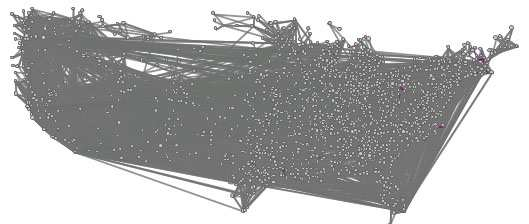
\includegraphics[width=100mm]{../figuras/cluttered-map.png}
  \caption[Trajetórias de voos nos Estados Unidos]{Trajetórias de voos nos Estados Unidos no período de uma semana. Fonte \citet{Zhou2013}.}
  \label{fig:exemplo-oclusao}
\end{figure}

  Algumas aplicações existentes no domínio do trânsito, como Google
Maps\footnote{\rurl{maps.google.com}} e
Waze\footnote{\rurl{www.waze.com/pt-BR}}, que sugerem para motoristas qual
caminho tomar até um determinado destino, e
OlhoVivo\footnote{\rurl{olhovivo.sptrans.com.br}}, que  mostra as rotas feitas
por ônibus na cidade de São Paulo e suas posições instantâneas, se empenham em
mostrar informações pontuais do tráfego e não na sua estrutura geral como um
todo. Para essa tarefa, precisariam ainda buscar soluções para contornar os
problemas de oclusão decorrentes da visualização de uma grande quantidade de
dados. O Google Maps, por exemplo, sugere um trajeto entre uma origem e um
destino inseridos pelo usuário e traça o percurso em um mapa. Sua visualização
destaca também as áreas com maior densidade de fluxo com diferentes cores,
sendo laranja trechos com fluxo moderado e vermelho sendo trechos de maior
fluxo, indicando que há um congestionamento. A Figura \ref{fig:gmaps} ilustra
uma visualização de uma rota sugerida pelo Google Maps. Podemos imaginar como
seria visualizar todas os trajetos pesquisados em um dia e que tipo de problema
teríamos.

\begin{figure}[!htb]
  \centering
  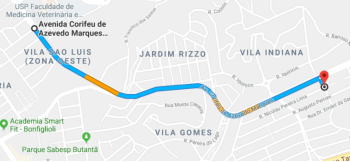
\includegraphics[width=\textwidth]{../figuras/maps.pdf}
  \caption{Trajeto entre dois pontos visto com o Google Maps \label{fig:gmaps}}
\end{figure}

  Para lidar com os problemas da oclusão, algumas técnicas têm sido
desenvolvidas por comunidades de visualização e da cartografia para a o estudo
de grandes conjuntos de dados de tráfego, como por exemplo, clusterização de
vértices \citep{Schaeffer2007,Andrienko2011}, matrizes \citep{Elmqvist2008}
e grides \citep{JoWood2010}. Essas técnicas, no entanto, acabam usando
abstrações diferentes da representação baseada em linhas. Um outro tipo de
abstração pode ser obtido com uma técnica chamada \emph{bundling}, que tem sido
bastante utilizada na visualização massiva de dados do tráfego que utilizam a
representação de fluxos por linhas \citep{Zhou2013}. Algoritmos de
\emph{bundling} agrupam arestas similares e próximas, permitindo uma
representação única e compacta que reduz o número de arestas e a oclusão no
desenho. A Figura \ref{fig:exemplo-bund} ilustra a aplicação da técnica de
\emph{bundling}.  Quanto mais à esquerda, mais oclusão, e à direita, o
resultado final.

\begin{figure}[!htb]
  \centering
  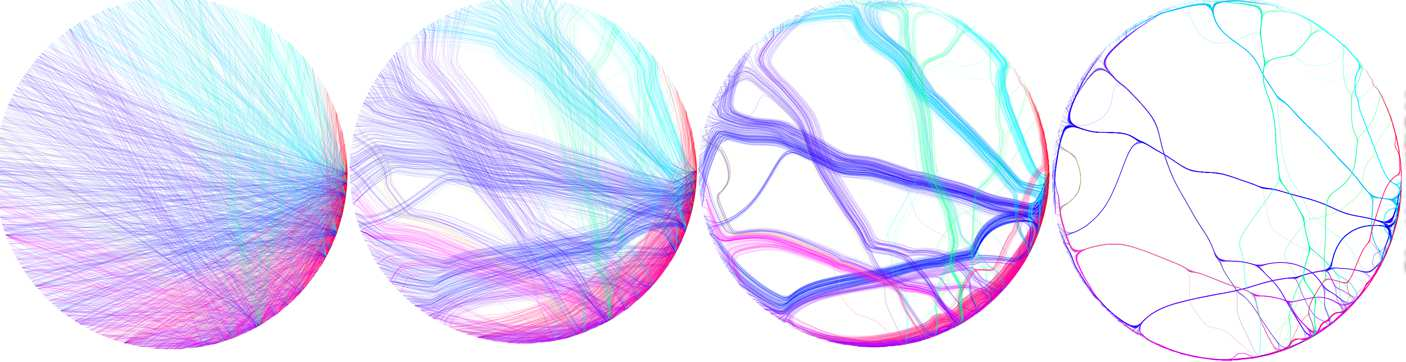
\includegraphics[width=1\textwidth]{../figuras/bundle-ex.png}
\caption[Exemplo de aplicação do \emph{bundling}]{Exemplo de aplicação do \emph{bundling}. Fonte: \citet{Hurter2012}.}
  \label{fig:exemplo-bund}
\end{figure}

  Uma variedade de métodos de \emph{bundling} têm sido apresentados por
pesquisadores, como métodos geométricos, hierárquicos e baseados em imagem
\citep{Lhuillier2017}. Recentemente, novos métodos viabilizaram a visualização
de grandes conjuntos de dados e em diferentes níveis de detalhes, como em
\citet{Klein2014}, que utilizam \emph{bundling} na visualização de milhares de
dados do tráfego aéreo. Eles mostram como a técnica destaca rotas comuns nos
voos e o grau de conexão entre diferentes aeroportos. O método utilizado
permite ainda uma abordagem multinível de acordo com parâmetros que
possibilitam o controle do \emph{bundling} em função da densidade de pontos no
espaço. Isso significa que é possível visualizar padrões globais entre grandes
áreas no mapa, que contemplem muitos pontos, e também padrões locais sobre
áreas menores com poucos pontos. Os autores também apresentam uma visualização
dinâmica para mostrar as mudanças no tráfego ao longo do tempo, agrupando os
voos em pequenos intervalos de tempo $\Delta t$ e aplicando o \emph{bundling}
nos dados de cada intervalo.

  Neste trabalho, focamos na visualização do fluxo de veículos no trânsito e as
relações de origem-destino (OD) que eles representam. Apresentamos uma
visualização dos dados utilizando \emph{bundling} para explorar os fluxos de
deslocamentos no trânsito da cidade e como eles impactam em vias com grandes
congestionamentos. Fazemos um novo estudo sobre visualização de dados do
tráfego projetando uma visualização para mostrar os fluxos em diferentes níveis
de detalhe. Utilizamos dados do tráfego de ônibus na cidade de São Paulo e
também dados gerados pelo InterSCSimulator, um simulador de cidades
inteligentes apresentado por \citet{mabs2017}.

\section{Objetivos e Contribuições}
  O objetivo desta pesquisa é explorar como o \emph{bundling} ajuda na
observação de padrões nos fluxos de deslocamento no tráfego de veículos de uma
grande cidade. Para isso, fazemos uma análise sobre as propriedades temporais e
espaciais dos dados do tráfego, sendo a direção e a densidade os principais
atributos que utilizaremos para responder às seguintes questões de pesquisa:

\begin{itemize}
  \item \textbf{Q1:} Como o \emph{bundling} pode ser usado para identificar os
fluxos de origem e destino no trânsito em diferentes escalas?

  \item \textbf{Q2:} Como o \emph{bundling} pode ser usado para identificar
mudanças no tráfego em horários de pico e outros horários do dia, e também na
ocorrência de eventos atípicos como fechamento de uma rua com grande fluxo?

  \item \textbf{Q3:} Como é o desempenho computacional do \emph{bundling} na
visualização de uma grande quantidade de dados do trânsito?
\end{itemize}

 Para isso, apresentamos o InterSCityPlotter, uma ferramenta livre e de código
aberto, para a análise de dados do tráfego de veículos que utiliza
\emph{bundling} para visualização dos dados do trânsito.  Exploramos o
\emph{bundling} em três aspectos: (1) abordagem multinível para visualizar
padrões globais (i.e. na escala da cidade), e locais (i.e. bairros, quadras e
ruas); (2) abordagem dinâmica para visualização de mudanças no padrão de fluxos
ao longo do tempo; (3) sua utilização com uma grande quantidade de dados do
trânsito em escala real de uma grande cidade, com mais de 4 milhões de
veículos.  Apresentamos também um conjunto de técnicas para mapear os atributos
de direção e densidade dos dados dentro de uma visualização sobre um mapa.

  Avaliaremos os resultados da visualização de maneira qualitativa e
quantitativa. Do ponto de vista qualitativo avaliaremos o que foi alcançado com
a visualização em relação às questões \textbf{Q1}, \textbf{Q2}, \textbf{Q3} e
\textbf{Q4} levantadas, fazendo considerações sobre suas vantagens e
desvantagens. Além disso, compararemos nossa proposta em relação a outros
trabalhos sobre visualização de dados de movimentação que utilizam
\emph{bundling}. Do ponto de vista quantitativo será avaliado o desempenho da
solução dado o tempo de processamento para gerar a visualização dos conjuntos
de dados utilizados.

  Esperamos que a visualização a ser criada ajude na identificação das relações
entre as regiões da cidade que recebem maior fluxo, como esse fluxo se
distribui ao longo do tempo e como ele impacta em vias com grandes
congestionamentos. Desta forma, esta pesquisa potencialmente oferece as
seguintes contribuições científicas (CC) e contribuições técnicas (CT):

\begin{itemize}
  \item \textbf{CC} - avaliação do \emph{bundling} em multiníveis para análise de
padrões globais e locais do tráfego

  \item \textbf{CC} - avaliação da escalabilidade do \emph{bundling} na visualização de uma grande
quantidade de dados do tráfego de veículos

  \item \textbf{CC} - avaliação do \emph{bundling} dinâmico para análise de mudanças ao longo
e a ocorrência de eventos atípicos

  \item \textbf{CT} - construção de uma ferramenta para visualização dos dados do tráfego
que será integrada ao InterSCSimulator
\end{itemize}

Esta pesquisa está sendo desenvolvida como parte do projeto InterSCity
\footnote{\rurl{interscity.org}} - INCT of the Future Internet for Smart
Cities. O objetivo do projeto é desenvolver pesquisas multidisciplinares em
infraestruturas de software para cidades inteligentes, produzindo contribuições
técnicas e científicas para a comunidade \citep{Daniel2016}. O simulador InterSCSimulator foi
desenvolvido no contexto do projeto e nós nos apoiamos em seus resultados como
forma de impulsionar esta pesquisa no campo da visualização de dados do
tráfego. Desta forma, o desenvolvimento desta pesquisa de mestrado seguirá as
diretrizes do projeto InterSCity para produzir resultados que sejam
reprodutíveis, bem como soluções de software livre que possam ser mantidas
adiante pela comunidade do projeto.

\par
%Falar sobre visualização de dados. Visualização de dados de origem e destino.
%Multi atributos. Multiplas origem e destinos. Representação geoespacial.
%Multi atributos. Propomos uma visualização que utiliza bundling, cores e filtros
%para explorar dados geoespaciais em uma grande cidade. Exploramos a visualização
%em vários aspectos desse cenário complexo (correlação, filtragem de dados, cores)
%e mostramos como ela se comporta para mostrar características dos dados de
%origem-destino, além de parâmetros e peculiaridades do modelo de bundling escolhido.
%Por exemplo, mostramos regiões contém maior fluxo filtrando por
%diferentes modais de transporte. Mostramos a correlação entre renda e modais
%para mostrar que pobre é quem anda a pé e mora longe. Além de calcular como
%é o fluxo no tempo utilizando cores, filtros e subtração de dados para observar
%a evolução ao longo do dia e ao longo dos anos. Apresentamos também os aspectos
%de escalabilidade computacional da técnica, dissertando sobre a complexidade
%do algoritmo nos cenários medindo ainda os tempos de execução.

\chapter{Referencial teórico}
\label{cap:referencial-teorico}

  Neste capítulo esclarecemos os conceitos teóricos necessários para o
entendimento do trabalho e a metodologia proposta. Inicialmente, abordamos
aspectos da visualização de dados do tráfego, que abrange uma variedade de
cenários conforme os objetivos, tipos de dado e diferentes representações
visuais da informação. Neste contexto, destacamos o \emph{bundling}, uma
técnica bastante usada na visualização de grandes quantidades de dados do
tráfego. Apresentamos os detalhes da técnica e uma breve consideração sobre os
avanços recentes nesta área. Por fim, considerando que neste trabalho faremos o
uso de dados simulados do tráfego de veículos, apresentamos o simulador
InterSCSimulator.

\section{Visualização de dados do tráfego}

  A análise de dados do tráfego tem um histórico antigo. \citet{Chen2015} fazem
um levantamento de várias pesquisas de análise e visualização de dados do
tráfego de pessoas, carros e embarcações. Eles apresentam uma taxonomia
conforme algumas características observadas, como o objetivo da visualização,
formato dos dados do tráfego e formas de apresentação de suas propriedades.
Nesta seção apresentamos essa taxonomia, que é importante para um melhor
entendimento da área e dos esforços que têm sido feitos no campo da
visualização de dados do tráfego.

\subsection{Quanto ao Objetivo da Visualização}

  Segundo \citet{Chen2015}, os trabalhos e sistemas de software sobre análise e
visualização de dados do tráfego podem ser classificadas em quatro categorias
de acordo com seus objetivos e a tarefa a que servem.

\begin{description}
  \item[Monitoramento do tráfego:] esse tipo de aplicação
foca no monitoramento em tempo real para descobertas instantâneas de eventos no
tráfego, como câmeras de gravação ao vivo e sistemas de alerta.

  \item[Descoberta de padrões e clusterização:] para a descoberta de padrões e
tendências de mobilidade, algumas aplicações utilizam métodos para o
agrupamento visual de trajetórias ou novas abstrações dos dados.

  \item[Exploração e predição:] outras aplicações focam em fornecer mecanismos
de pesquisa e exploração dos dados para que os usuários investiguem os dados
que justifiquem situações do tráfego, como congestionamentos, ou ainda técnicas
de predição para prever essas situações (e.g. predizer que haverá
congestionamento devido a ocorrência de chuva).

  \item[Planejamento de rotas e recomendação:] sistemas de transporte
inteligentes contam essencialmente com recomendações de trajetos para usuários
do transporte, várias soluções existem com esse propósito, que podem envolver monitoramento
em tempo real ou análise histórica no processo de recomendação.
\end{description}

\subsection{Quanto ao Tipo de Coleta dos Dados}

  Dados do tráfego são tipicamente coletados a partir de sensores e dispositivos
eletrônicos. A estrutura desses conjuntos de dados dependem do modo de operação
dos sensores e dispositivos que registram a movimentação dos objetos. \citet{Chen2015}
os dividem em três classes:

\begin{description}
  \item[Baseado em pontos de interesse:] a posição de um objeto é gravada assim
que ele entra na área do sensor. Como uma câmera de vídeo que capta a
movimentação e orientação de um veículo assim que ele passa pela área de
monitoramento.

  \item[Baseado em ações:] as informações sobre um objeto podem estar associados
a certas atividades. O usuário de um aparelho celular por exemplo, tem sua
atividade e localização registrados pela rede GSM quando o mesmo efetua uma
chamada.

  \item[Baseado em sinais de dispositivos:] Um dispositivo de localização
carregado por um objeto constantemente grava e envia suas informações de
localização para uma central, como aparelhos de GPS instalados em um ônibus do
transporte público de uma cidade.  \end{description}

  Uma série de posições de localização ao longo do tempo formam a trajetória de
um objeto. Uma trajetória contém informações temporais, que permitem traçar uma
linha do tempo da movimentação, e informações espaciais, que contém a posição
em cada momento no tempo. A frequência de armazenamento dessas informações
também impacta a análise. Capturar e armazenar essas informações com um
intervalo de tempo muito pequeno pode ser algo bastante custoso. Outro fator de
impacto é a precisão das informações a qual depende de questões relacionadas ao
hardware utilizado na coleta. Muitas vezes é necessária uma etapa de
pré-processamento para extrair dados inconsistentes da análise.

\subsection {Visualização das Propriedades Temporais}
\label{sec:prop-espaciais}

  Dados do tráfego podem conter uma série de variáveis, das quais as mais
importantes são o tempo e espaço. Visualizações orientadas ao tempo enfatizam
tendências, periodicidades e anomalias nos dados ao longo de um eixo temporal \citep{Aigner2008}.

  Expressar a variação do tráfego ao longo do tempo e sua evolução é um típico
processo de análise linear do tempo, que é considerado a partir de um ponto de
início até um ponto final \citep{Chen2015}. Por exemplo, em um gráfico de
linhas, o tempo é representado ao longo do eixo X e outra variável é
representada no eixo Y, como na Figura \ref{fig:linear-time}. Gráficos de
linhas são fáceis de interpretar, porém limitam-se na quantidade de variáveis
que podem ser visualizadas.

\begin{figure}[!htb]
  \centering
  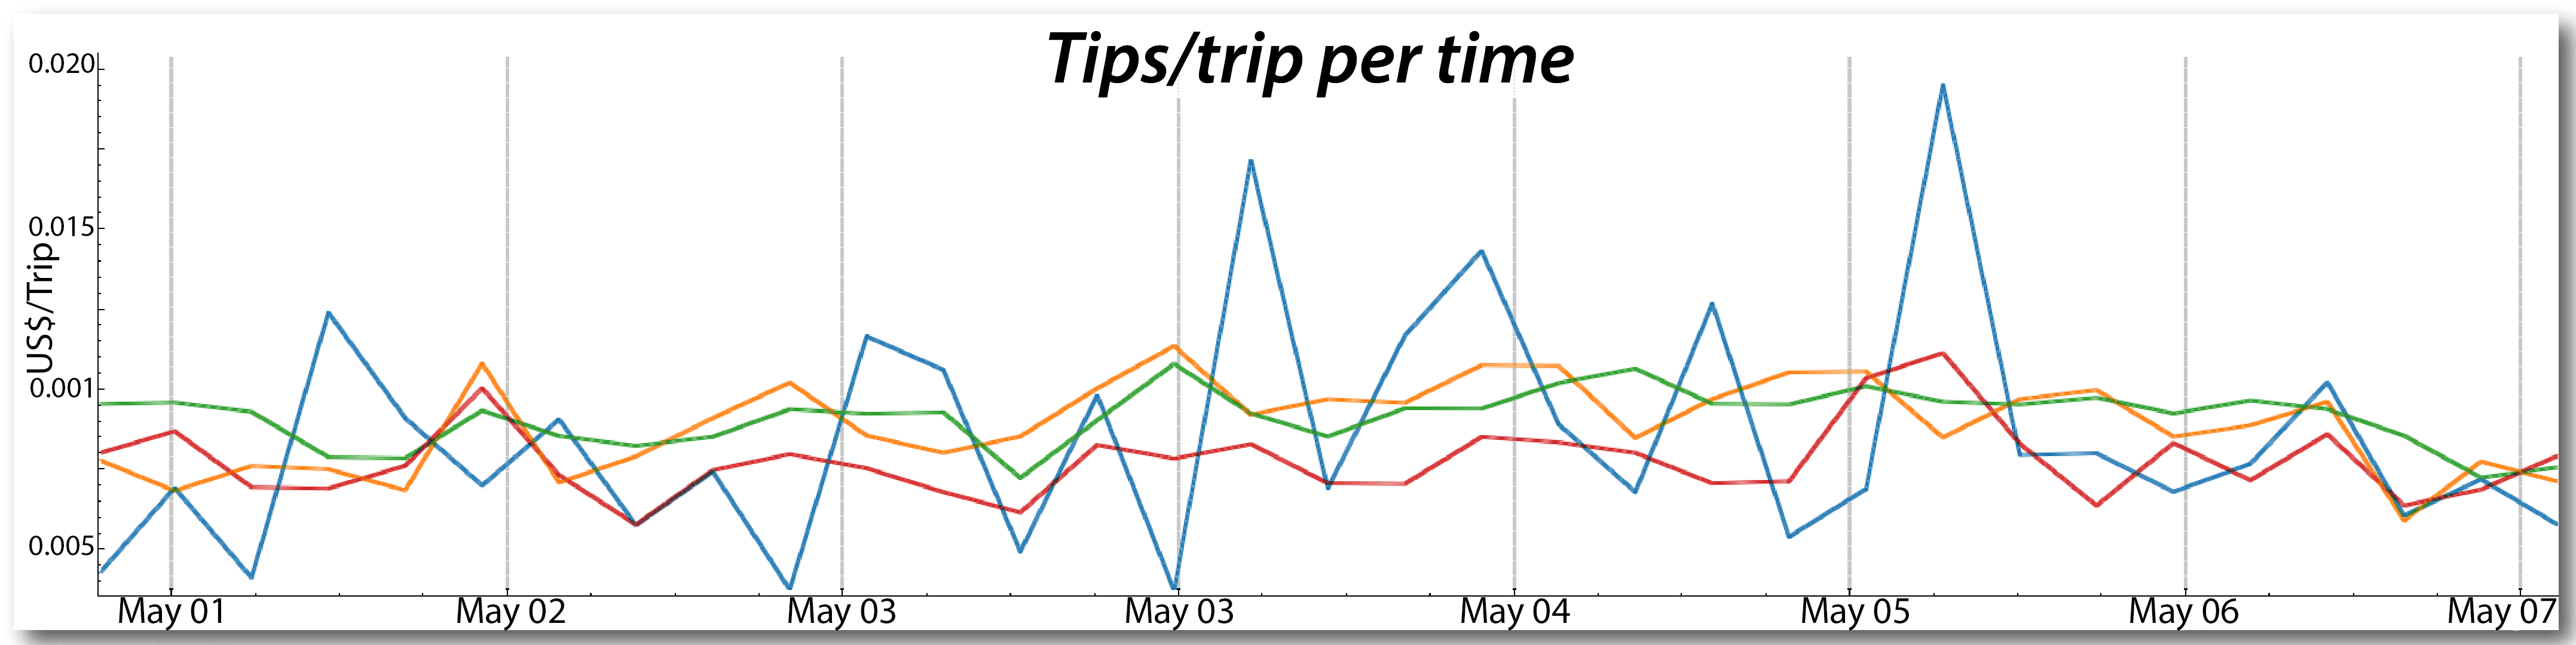
\includegraphics[width=\textwidth]{../figuras/linear-time.png}
  \caption[Gráfico de linha representando empo linear]{Gráfico de linha representando tempo linear. Ele mostra a média de gorjetas por viagem em diferentes regiões no período de 1 a 7 de Maio de 2011. Cada linha representa uma região. Fonte: \citep{Ferreira2013}
  \label{fig:linear-time}}
\end{figure}

  Por outro lado, temos também alguns processos recorrentes que são naturais em
nosso mundo, os quais seguem ciclos de estações, ou mesmo ciclos semanais e
diários. Um leiaute radial visto na Figura \ref{fig:periodic-time} é uma opção
para se visualizar essa periodicidade. O tempo é mostrado no eixo circular e
cada anel do círculo representa um dia da semana.  Os setores representam uma
hora, com 24 setores no total que mostram a quantidade de tráfego em um
determinado ponto da cidade, mapeada em cores. A vantagem de um leiaute radial
é que ele evidencia esses padrões recorrentes e a desvantagem é que ele possui
pouca eficiência espacial \citep{Chen2015}.

\begin{figure}[!htb]
  \centering
  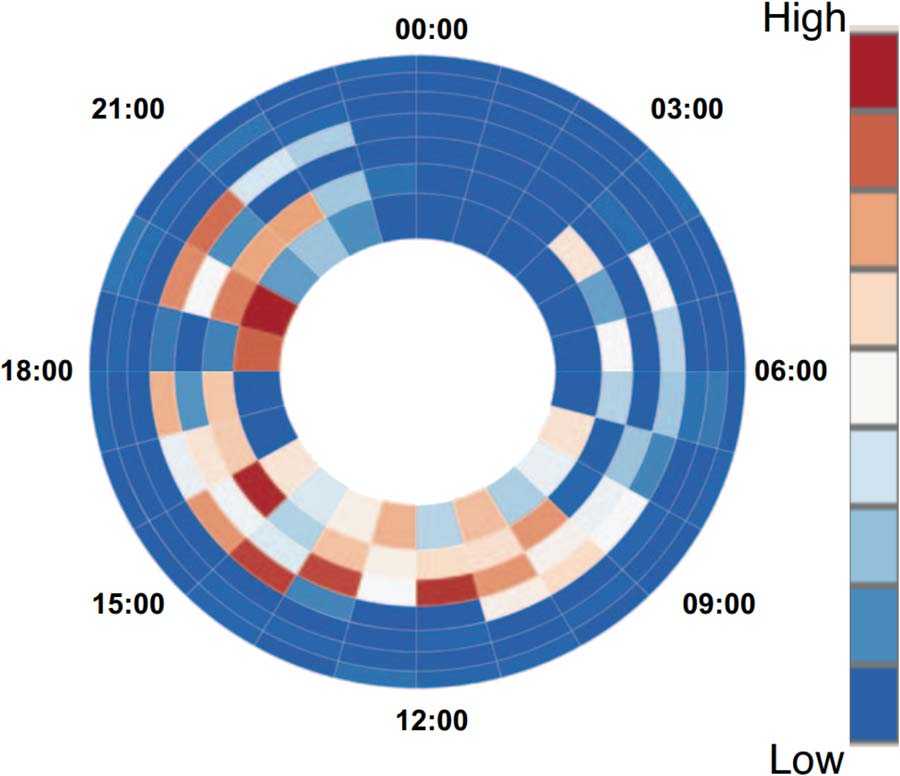
\includegraphics[width=0.6\textwidth]{../figuras/periodic-time.png}
  \caption[Leiaute radial representando tempo periódico]{Leiaute radial
representando tempo periódico. O tempo é mostrado no eixo circular e cada anel
do círculo representa um dia da semana, divididos em 24 setores que indicam as
24 horas do dia. As cores mostram a quantidade de tráfego conforme o mapa à
direita, onde vermelho maior é o tráfego. Fonte:
\citet{Pu2013} \label{fig:periodic-time}}
\end{figure}

  Os aspectos temporais dos dados não se limitam a apenas essas visualizações,
existe um grande arcabouço de projeções que se desenvolveram no campo da
visualização da informação onde o tempo é uma variável de destaque,
\citet{Cairo2016} mostra uma série dessas projeções em seu livro. Uma análise
linear ou periódica são dois paradigmas que levam a decisões diferentes durante
o processo de criação da visualização.

\subsection{Visualização das propriedades espaciais}

  As propriedades espaciais de localização referem-se aos locais onde ações,
incidentes e eventos ocorrem. Diferentes níveis de agregação dessa informação
levam à categorização da visualização em três classes, segundo
\citet{Chen2015}: visualização baseada em pontos (nenhuma agregação),
visualização baseada em linhas (agregação de primeira ordem), e agregação
baseada em regiões (agregação de segunda ordem).

\begin{description}
  \item[Visualização baseada em pontos:] visualizações baseadas em pontos
consideram as informações do tráfego como pontos discretos e usam sua forma
pura como representação em um leiaute espacial, como por exemplo pontos em um mapa 2D. Essa técnica
mostra intuitivamente a posição de objetos em um certo momento no tempo. O
projeto \emph{Trains of Data}, ilustrado na Figura \ref{fig:trains-of-data},
utiliza esse tipo de visualização para representar a movimentação dos trens na
França. O tamanho dos pontos indica a quantidade de passageiros e a cor indica
se o trem está atrasado, sendo verde no horário e vermelho significa atraso.
Para uma visualização integral da trajetória eles ainda usam efeitos de
animação. Visualizações baseadas em pontos tipicamente representam cada ponto
de forma individual. Em casos onde há uma grande quantidade de pontos, o uso de
mapas de calor é indicado para a visualização da densidade. A vantagem desse
método é que ele permite observar os estados de cada objeto e sua distribuição
no espaço, como também explorar regiões da cidade que estejam mais ocupadas.
Por outro lado, ele é inapropriado para representação de informações contínuas,
como quantos veículos viajam de um determinado local para outro.

\begin{figure}[!htb]
  \centering
  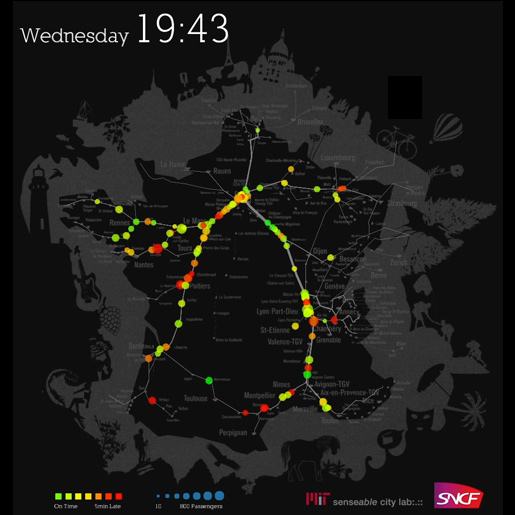
\includegraphics[width=.6\textwidth]{../figuras/trains-of-data.jpg}
  \caption[Visualização baseada no mapa das ferrovias da França]{Posição dos trens às 19:43 na França com uma visualização baseada no mapa
das ferrovias. Fonte: \citet{Senseable2018}.}
  \label{fig:trains-of-data}
\end{figure}

  \item[Visualização baseada em linhas:] visualizações baseadas em linhas são
desenhadas para mostrar a trajetória de objetos, mapas de vias e estradas em
uma região, ou fluxos do tráfego em uma rede de transporte. As trajetórias e
fluxos são representados por linhas ou curvas e são escaladas ou coloridas de
acordo com suas propriedades (i.e. densidade, direção, velocidade).
\citet{Klein2013} apresenta um sistema iterativo para análise do tráfego aéreo
na França. Cada trajetória é representada por uma linha que conecta os pontos
de partida e chegada de cada voo, como pode ser visto na Figura
\ref{fig:air-traffic}.

\begin{figure}[!htb]
  \centering
  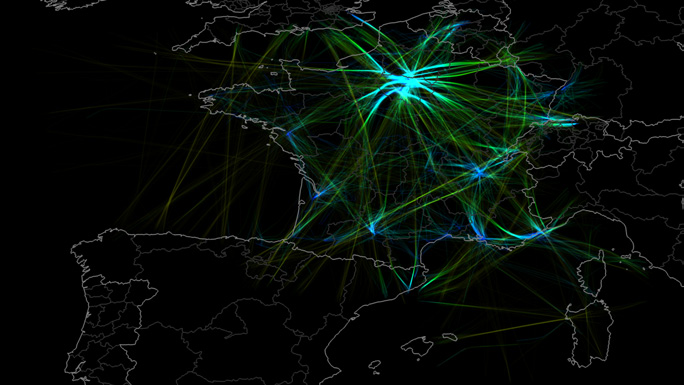
\includegraphics[width=1\textwidth]{../figuras/air-traffic.png}
  \caption[Visualização do tráfego aéreo na França]{Visualização do tráfego aéreo na França. Fonte: \citet{Klein2013}.}
  \label{fig:air-traffic}
\end{figure}

  A representação espacial das linhas pode ainda sofrer transformações
geométricas e topológicas que geram novas abstrações. Por exemplo,
\citet{Tarik2009} mostram uma proposta que transforma as trajetórias de um
leiaute espacial (Figura \ref{fig:viz-espacial}) para um leiaute abstrato
(Figura \ref{fig:viz-abstrata}) para visualizar a movimentação de pessoas
durante a fuga de uma explosão em um escritório.  A abordagem abstrata é usada
para mostrar mais efetivamente os padrões de movimentação de pessoas que se
movem ao mesmo tempo para as mesmas áreas. Na Figura \ref{fig:viz-abstrata} é
possível notar a movimentação de indivíduos antes da explosão (linhas azuis), o
que sugere possíveis suspeitos ou testemunhas do evento.  As informações
temporais são difíceis de representar no leiaute espacial, assim o leiaute
abstrato complementa a visualização dos dados mostrando os instantes de tempo
no eixo X e as informações espaciais no eixo Y.

\begin{figure}[ht!]
  \centering
  \begin{subfigure}[t]{0.45\textwidth}
    \centering
    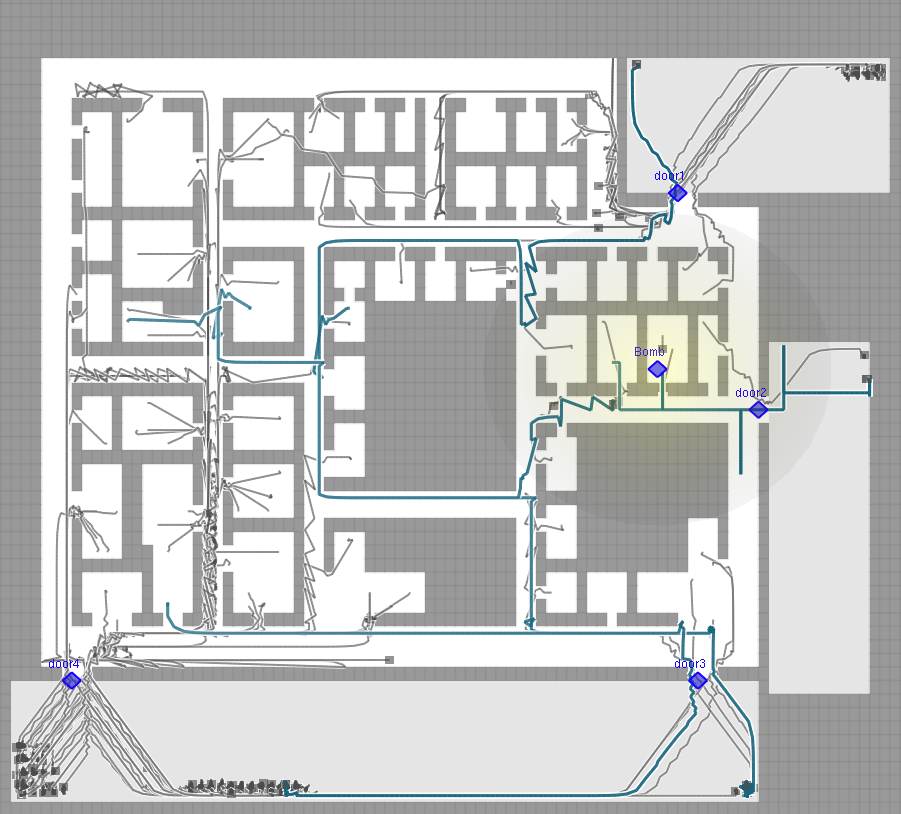
\includegraphics[width=65mm]{../figuras/proximidade-espacial.png}
    \caption{Visualização espacial das trajetórias ao longo do tempo. \label{fig:viz-espacial}}
  \end{subfigure}
  ~
  \begin{subfigure}[t]{0.45\textwidth}
    \centering
    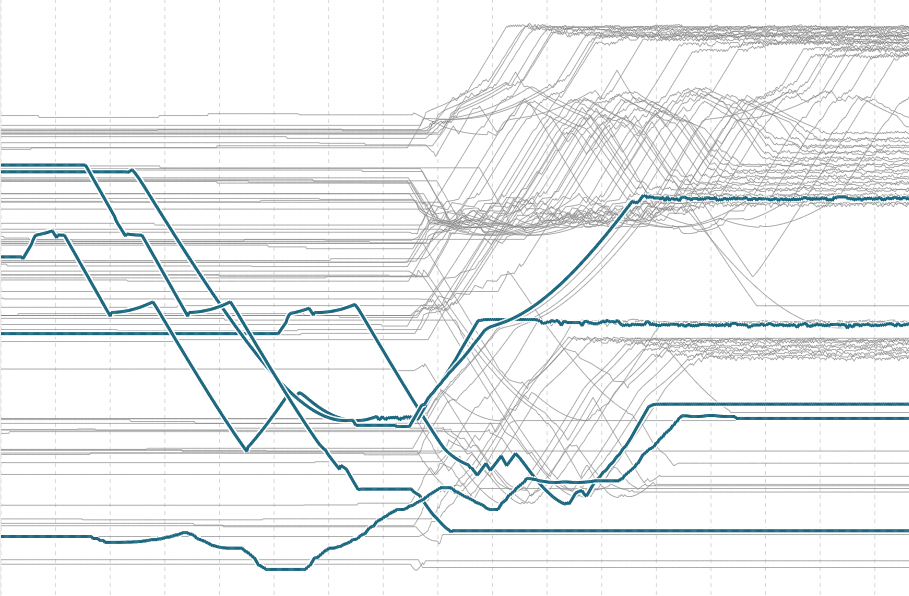
\includegraphics[width=75mm]{../figuras/proximidade-abstrata.png}
    \caption{Visualização abstrata da movimentação ao longo do tempo. \label{fig:viz-abstrata}}
  \end{subfigure}

  \caption[Visualização espacial vs abstrata da movimentação de pessoas em um
escritório]{Simulação de uma evacuação de um escritório depois de uma explosão.
(a) Visualização da movimentação da trajetória das pessoas no espaço. (b)
Visualização abstrata, baseada na proximidade.  Fonte: \citet{Tarik2009}.
\label{fig:tarik}}
\end{figure}

%  Algumas ideias buscam ainda sintetizar as informações espaciais e temporais
%em um cubo espaço-temporal, que utiliza o eixo Z para mostrar o tempo e os
%eixos X e Y para representar o espaço. 

  No entanto, a medida que o número de objetos cresce, aumenta também os
problemas de oclusão, o que acaba afetando a estética da visualização e a
obtenção de informações sobre os dados \citep{Zhou2013}. Uma forma de reduzir
a complexidade de análise de um grande conjunto  trajetórias é utilizando
outras formas de abstração dos dados, como uma visualização baseada em regiões.

  \item[Visualização baseada em regiões:] Esse tipo de abstração agrupa fluxos
de deslocamento com origem e destino similares em um nível de macro regiões,
geralmente determinado por divisões administrativas.  \citet{Zeng2013}
apresentam um diagrama em círculos para mostrar padrões de movimentação de
pessoas entre as regiões da cidade. O círculo representa a junção ou conexão
entre as diferentes regiões e o fluxo entre elas. A densidade do fluxo é medido
pela espessura, bem como a direção é destacada dentro do círculo, como é
ilustrado na Figura \ref{fig:interchange-circo}. Apesar de facilitar a
visualização, esse tipo de agregação abre mão das informações individuais de
cada trajetória em favor de uma visão condensada dos fluxos.

\begin{figure}[!htb]
  \centering
  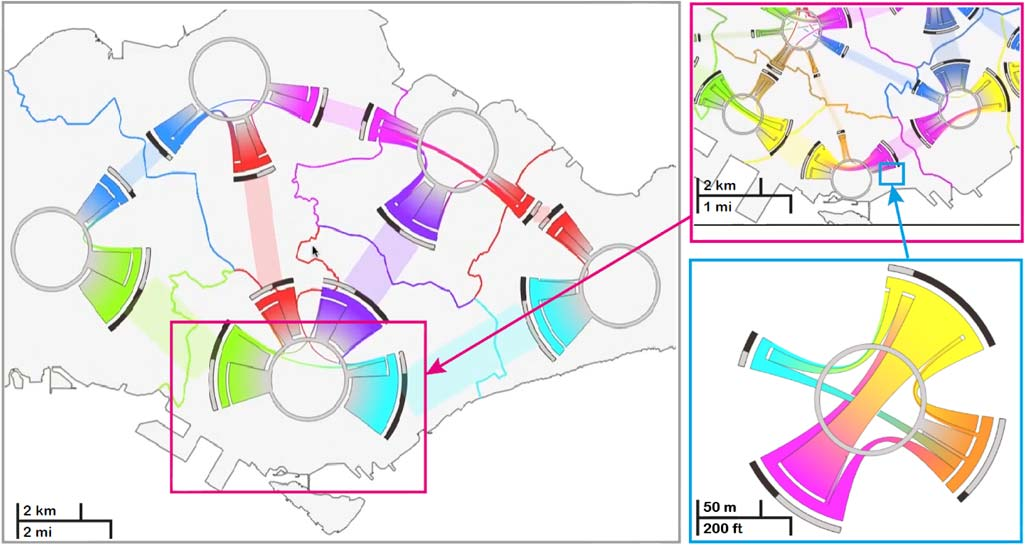
\includegraphics[width=1\textwidth]{../figuras/region-based.png}
  \caption[Exemplo de visualização baseada em regiões do sistema de metrô na França]{Exemplo de visualização baseada em regiões: padrões regionais de movimentação no sistema de metrô na França. Fonte: \citet{Zeng2013}.}
  \label{fig:interchange-circo}
\end{figure}
\end{description}

\section{\emph{Bundling}}
\label{sec:bundling}

  Um grande problema na visualização de grafos e dados de trajetórias é a
oclusão visual à medida que a quantidade de elementos aumenta. Uma pequena
quantidade de dados já começa a apresentar problemas de sobreposição e
cruzamento de arestas, o que dificulta a obtenção de informação sobre os dados.
Uma maneira de contornar esse problema é através de filtros que determinam a
quantidade de itens na visualização. Como consequência do filtro perde-se a
visão global de todos os itens ao mesmo tempo, o que pode ser necessário para a
identificação das correlações e padrões entre eles. Uma outra abordagem é o uso
de agregações que geram novas abstrações dos dados. Na seção anterior mostramos
como o agrupamento em regiões projetado sobre um diagrama circular simplifica a
visualização das trajetórias entre as áreas da cidade.

 Uma solução que tem sido amplamente utilizada em várias pesquisas de
visualização de dados de tráfego é o uso de uma técnica chamada
\emph{bundling}. A técnica ajuda a simplificar o desenho da visualização
através da agregação espacial das arestas em conjuntos chamados
\emph{bundles}, que funcionam de forma similar a algoritmos de clusterização. Os \emph{bundles} são
definidos como um grupo de arestas similares, compatíveis o suficiente para
serem representadas por um corpo único e compacto \citep{Lhuillier2017}. A
compatibilidade é calculada a partir de uma função de similaridade usada para
determinar quais arestas devem fazem parte do mesmo agrupamento.
Imaginando então algumas viagens no trânsito, podemos agrupá-las pela sua
região de origem, destino, distância percorrida, direção ou até mesmo o meio de
transporte utilizado.  Dessa forma, o número de \emph{bundles} é ligeiramente
inferior ao número de trajetórias a serem desenhadas, ficando mais simples
compreender e visualizar a estrutura global, padrões e tendências entre grupos
de trajetórias que ligam áreas fortemente relacionadas \citep{Zhou2013}.  A
Figura \ref{fig:bundling-hierarquico} mostra o uso de uma técnica de
\emph{bundling} para visualização da hierarquia de módulos e arquivos de um
software onde as arestas mostram suas relações de dependência. A ligação
acontece quando um módulo acessa atributos e/ou funções definidos em outras partes
do software.

\begin{figure}[!htb]
  \centering
  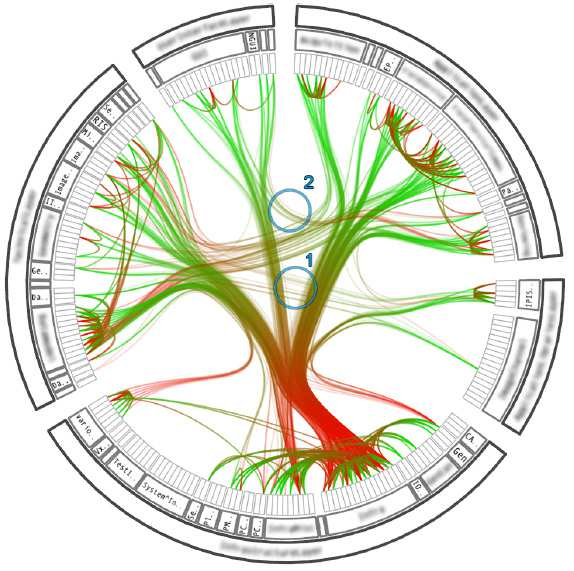
\includegraphics[width=.5\textwidth]{../figuras/hbundling.png}
  \caption[Bundling hierárquico na visualização de dados de software]{Bundling hierárquico na visualização de dados de software. As cores mapeiam
o sentido do acesso, verde é a origem, vermelho é o alvo. Fonte: \citep{Holten2006}.}
  \label{fig:bundling-hierarquico}
\end{figure}

\subsection{Modelos de \emph{Bundling}}

  O cálculo de um \emph{bundle} não possui uma definição precisa, e por isso há
uma grande variedade de algoritmos e abordagens para modelar problemas de
agrupamento de arestas com \emph{bundling}, que podem variar significativamente
de um para outro em questões de complexidade e aplicação dos algoritmos
\citep{Zhou2013}.  \emph{Force-directed edge bundling} (FDEB), apresentado em
\citet{Holten2009}, cria \emph{bundles} através da atração entre pontos de
controle colocados ao longo das arestas e é considerado um modelo baseado em
custo, já que tenta minimizar o valor de uma função de custo que representa a
força de atração entre as arestas.  \emph{Hierarchical Edge Bundling} (HEB)
agrupa as arestas baseadas na estrutura hierárquica do grafo para o cálculo dos
\emph{bundles} e por isso é considerado um modelo geométrico \citep{Holten2006}. Outra
classificação são os modelos baseados em imagem, como \emph{Skeleton-based edge
bundling} (SBEB) e \emph{Kernel Density Estimation-based Edge Bundling}
(KDEEB), que surgiram mais recentemente. Eles utilizam algoritmos de
clusterização para extrair a estrutura geral do grafo para então calcularem os
\emph{bundles}. O algoritmo SBED utiliza o esqueleto do grafo como guias para
criar \emph{bundles} com muitas ramificações \citep{Ersoy2011}, enquanto o
KDEEB utiliza um mapa de densidade do grafo para extrair sua estrutura no
espaço da imagem \citep{Hurter2012}. A Figura \ref{fig:subfigures} dá um
exemplo da variedade de possíveis saídas geradas por diferentes algoritmos de
\emph{bundling} (FDEB, SDEB e KDEEB) aplicados nos mesmos dados.  Nesse exemplo
são usados dados de uma semana do tráfego aéreo sobre os EUA.

\begin{figure}[!htb]
  \centering
  \begin{subfigure}{0.6\textwidth}
    \centering
    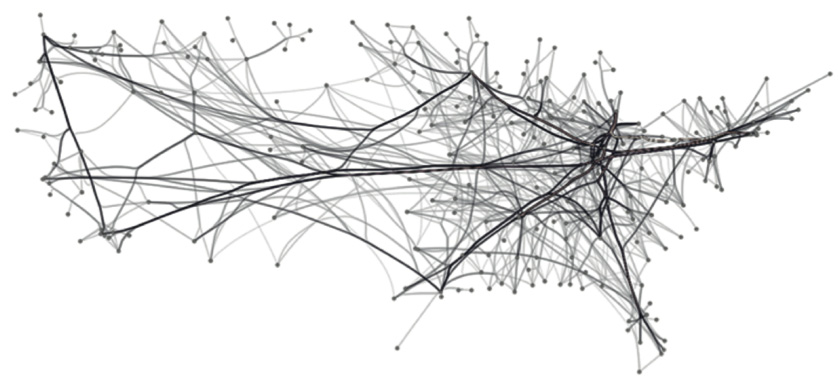
\includegraphics[width=1\textwidth]{../figuras/FDEB.png}
    \caption{FDEB}
    \label{fig:FDEB}
  \end{subfigure}

  \begin{subfigure}{0.6\textwidth}
    \centering
    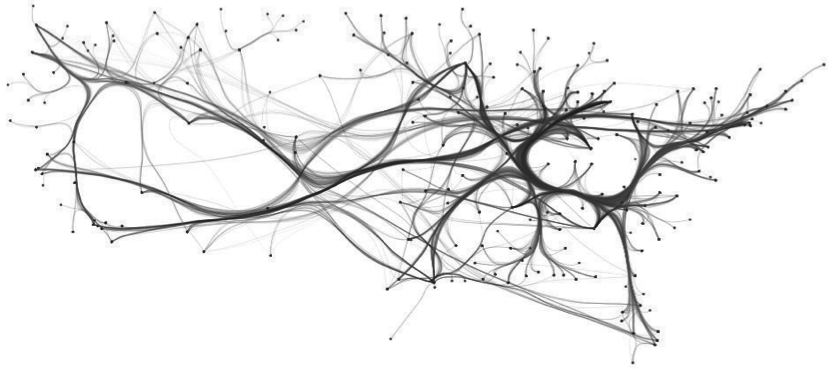
\includegraphics[width=1\textwidth]{../figuras/SBEB.png}
    \caption{SBEB}
    \label{fig:SBEB}
  \end{subfigure}

  \begin{subfigure}{0.6\textwidth}
    \centering
    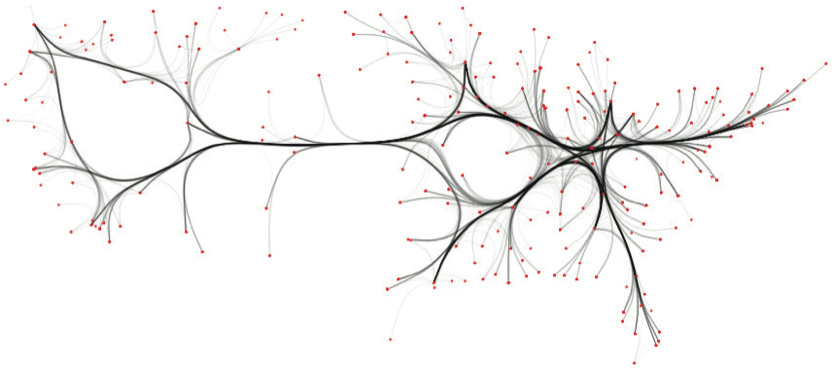
\includegraphics[width=1\textwidth]{../figuras/KDEEB.png}
    \caption{KDEEB}
    \label{fig:KDEEB}
  \end{subfigure}
  \caption[Diferentes algoritmos de \emph{bundling} aplicadas nos mesmos dados]{Diferentes algoritmos de \emph{bundling} aplicadas em dados do tráfego aéreo dos EUA - 235 nós, 2099 arestas. Fonte: \citep{Klein2013}.}
  \label{fig:subfigures}
\end{figure}

  A escolha do modelo geralmente parte da observação e experiências de
aplicação em problemas semelhantes, já que conhecer e testar diferentes
abordagens e suas variações não é uma tarefa simples. Por isso,
\citet{Lhuillier2017} recentemente propôs uma nova taxonomia para os modelos e
algoritmos de \emph{bundling} dividindo-os com base no tipo de dados em que se deseja
aplicar a técnica. Eles justificaram que desta forma pesquisadores e usuários
da técnica pudessem focar no seu contexto de aplicação e não em detalhes
específicos de implementação algorítmica. Seu estudo dividiu os modelos
existentes inicialmente em dois grupos, conforme o tipo de dados, grafos ou
trajetórias. Então, mais detalhes sobre a direção (direcionado ou não),
dimensão (2D ou 3D) e dependência do tempo (dinâmico ou estático) refinam a
divisão dentro da sua taxonomia.


\begin{figure}[!htb]
  \centering
  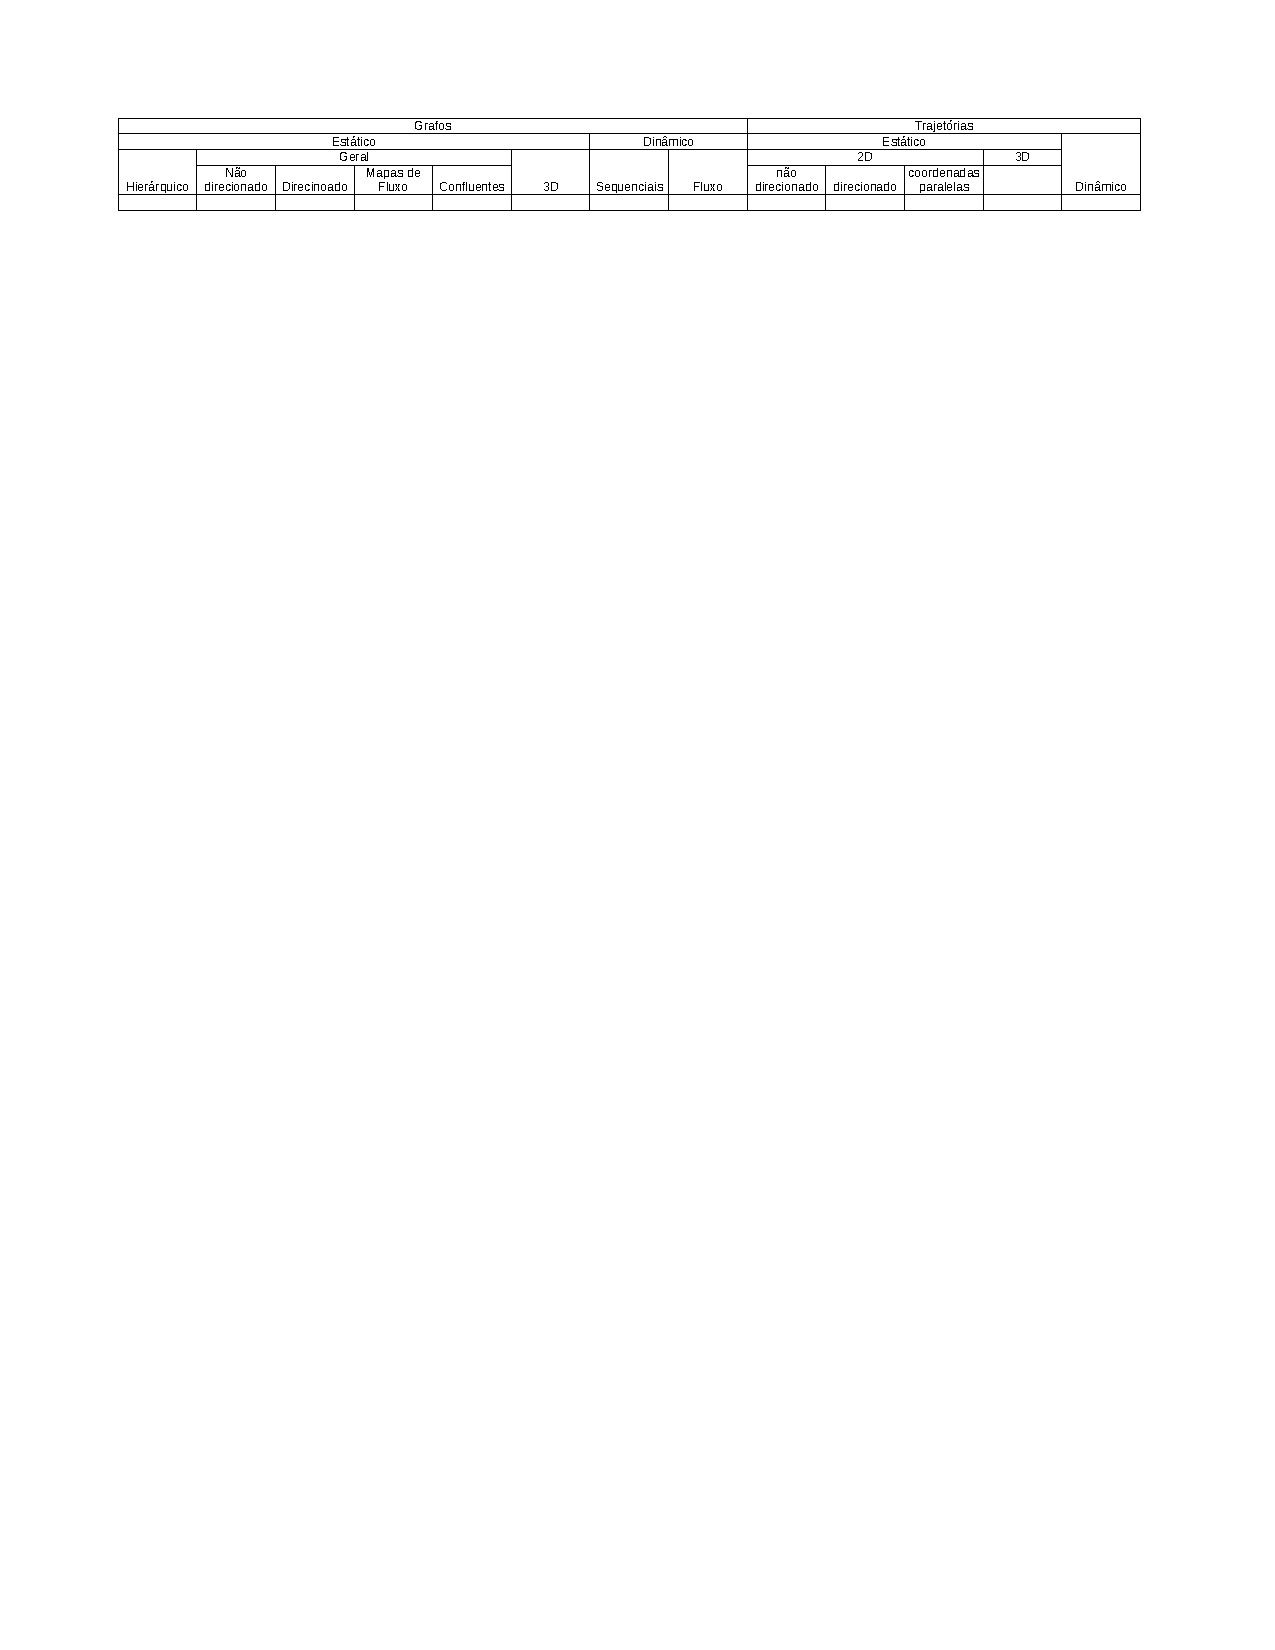
\includegraphics[width=\textwidth]{../figuras/estado-da-arte.pdf}
  \caption[Taxonomia dos métodos de \emph{bundling} baseado no tipo de dado]{Taxonomia dos métodos de \emph{bundling} baseado no tipo de dado. Fonte: \citet{Lhuillier2017}}
  \label{table:bundling-methods}
\end{figure}


Podemos então seguir a taxonomia para selecionar uma método de
\emph{bundling} que seja mais adequado para a análise de fluxos no trânsito da
cidade. \emph{Attribute-Driven Edge Bundling} (ADEB) é um algoritmo que segue um
modelo baseado em imagem e é apresentado dentro desta taxonomia como um das
opções para a análise de dados de trajetórias direcionadas. Discutimos na
próxima seção as características desse modelo e como podemos nos beneficiar
dele em nosso estudo.

\subsection{Modelo Baseado em Imagem}
\label{sec:modelo-imagem}

  Uma das etapas do \emph{bundling} é a identificação das trajetórias
similares, que requerem que cada uma delas seja comparada a todos os outras
para descobrir quais são as mais próximas, afim de agrupá-las em
\emph{bundles}.  Esse cálculo, no entanto, é bastante custoso e pode demorar
minutos em cenários com milhares de trajetórias.

\emph{Kernel Density Estimation Edge Bundling} (KDEEB) é um algoritmo proposto
por \citet{Hurter2012}. Eles observaram que ao aplicar uma operação de \emph{bundling} $B$ qualquer sobre um
grafo $G$, o resultado são áreas de maior densidade (dentro dos \emph{bundles})
e áreas de menor densidade fora deles, em comparação ao grafo original. Assim,
essa operação \emph{bundling} $B$ pode ser moldada em função de uma operação
sobre a densidade dos pontos do grafo, similar ao que faz o algoritmo de
clusterização \emph{Mean Shift} \citep{Comaniciu2012}. A partir disso, a heurística
desse algoritmo de \emph{bundling} consiste em computar repetidamente o
gradiente dos pontos em relação à uma função de densidade, e então movendo-os
para regiões mais densas apontadas pelo gradiente. O maior benefício do método
é sua implementação paralela com o uso do poder computacional de placas
gráficas (GPUs), o que levou a ganhos de desempenho de uma ordem de magnitude
em relação a métodos anteriores. KDEEB representou uma abertura para uma área
chamada \emph{image-based bundling}, ou métodos baseados em imagem, onde $B$ é
implementado via operações de processamento de imagem, diferentemente de
métodos puramente geométricos existentes até então. O algoritmo consiste nos
seguintes passos:

\begin{enumerate}
  \item Converte o grafo $G$ em um mapa de densidade usando uma função de
densidade. A função utilizada é um estimador baseado em núcleos, geralmente um
estimador Gaussiano ou Epanechnikov.

  \item Computar o gradiente da função de densidade para cada ponto/nó do
grafo. O cálculo do gradiente indica a direção onde há maior quantidade
de nós/arestas aglomeradas no grafo.

  \item Mover os nós na direção do gradiente (áreas mais densas). Essa etapa é
suavizada movendo-se os nós pela norma do gradiente, ou seja, em apenas uma unidade
a cada iteração. Isso evita que as arestas dêem grandes saltos.

  \item Corrigir distorções causadas pela movimentação dos nós com filtro
Laplaciano (opcional).  O passo anterior pode causar pequenas distorções, como
por exemplo, a sobreposição de nós. Esta é uma forma de se corrigir essas
distorções sem que se perca a estrutura geral do grafo.

  Repetir a partir do passo 1 até a convergência do algoritmo, o que leva cerca de 8..10
iterações.
\end{enumerate}

%\citet{Hurter2012} apresentam ainda uma maneira para limitar os \emph{bundles}
%com relação a obstáculos presentes no caminho das arestas. Um obstáculo
%qualquer, representado por seus limites espaciais pode ser contornado
%alterando-se a função de densidade, que sofre uma degradação dentro da área
%geométrica do obstáculo. Com isso, o gradiente age como uma força de repulsão
%das arestas que cruzam o obstáculo e faz com que as arestas sejam movidas
%na direção pra fora de suas bordas.

  {\emph{Attribute-Driven Edge Bundling} (ADEB) é uma extensão do algoritmo
KDEEB, proposta por \citet{ZegarraFlores2016}, e que permite a separação das
arestas conforme sua direção. Essa informação é obtida percorrendo cada aresta
a partir do ponto de origem até o destino e calculando para cada uma delas um
vetor unitário que aponta a sua direção, que é mapeado para o
ângulo desse mesmo vetor. Então, cria-se um mapa de densidade direcionado, onde são
consideradas apenas as arestas que vão na mesma direção (mesmo ângulo). Esse
algoritmo herda todos os benefícios de desempenho e robustez apresentados pelo
KDEEB, o que o faz um método adequado para a análise do tráfego de veículos no
trânsito da cidade.

\subsection{\emph{Bundling} em Dados Dinâmicos}

  Um grafo dinâmico é aquele no qual seus nós e arestas são dependentes do
tempo, ou seja, a cada momento \emph{t}, existe um grafo G(t) diferente a ser
explorado. Nesse contexto, dois diferentes tipos de grafos dinâmicos podem ser
considerados, grafos sequenciais e grafos de fluxo \citep{Hurter2013}. Um
grafo sequencial consiste em um conjunto de grafos $G^i = (V^i, E^i)$, onde
cada grafo $G^i$ é como um retrato no momento $i$ de um sistema que é
dependente do tempo. Grafos de fluxo, por outro lado, são definidos como um
conjunto de vértices $V$ e arestas $E$, onde as arestas são definidas pelo seu
tempo de vida e nós. Grafos de fluxo não possuem uma sequência pré-definida e
são tipicamente obtidos de fontes de dados online.

  O uso de \emph{bundling} nesse cenário é similar a outros métodos de
visualização de grafos dinâmicos. Para grafos sequenciais o \emph{bundling} é
aplicado a cada grafo $G^i$ de maneira estática. Já em grafos de fluxo, os
dados são divididos em janelas de tempo e o algoritmo é aplicado em cada
intervalo $\Delta t$, que podem ser colocados lado a lado para comparação em
uma técnica conhecida como \emph{small multiples}. Uma outra maneira de se
visualizar a dinâmica é com o uso de animações, como mostram
\citet{Hurter2014}. A vantagem desse método sobre o anterior é que ele se
adequa melhor à análise de longas séries temporais.

\section{Simulação do Tráfego de Veículos}

  O crescimento da população nas cidades ao redor do mundo trouxe também vários
desafios de gestão e controle do trânsito, especialmente em grandes cidades,
que precisam lidar com vários problemas de congestionamentos, acidentes,
poluição, controle do transporte público, entre outros. Uma maneira alternativa
para estudar e solucionar esses problemas é através do uso de ferramentas de
simulação. Essas ferramentas permitem criar cenários do tráfego de veículos e
ajudam nos estudos sobre seu comportamento e na elaboração de soluções para
serem aplicadas por gestores das cidades. Recentemente, novas ferramentas de
simulação com foco em escalabilidade foram desenvolvidas, permitindo testes e
experimentos em escala real de uma grande cidade, com milhões de veículos. O
InterSCSimulator é uma destas ferramentas e o detalhamos a seguir.

\subsection{InterSCSimulator}
\label{sec:interscsimulator}

\citet{mabs2017} apresentam o InterSCSimulator, uma ferramenta de código livre,
capaz de executar simulações com mais de 4 milhões de veículos em uma grande
metrópole.  As simulações são feita em escala mesoscópica. Isso significa que
ela segue um modelo onde cada veículo do trânsito é simulado individualmente. O
simulador calcula para cada um deles as ações de movimentação durante sua
viagem.

\subsubsection{Componentes do InterSCSimulator}

  O simulador possui quatro componentes principais: o \textbf{cenário}, que
recebe os arquivos de entrada e cria o grafo da cidade e os primeiros veículos;
\textbf{o motor de simulação}, que executa os algoritmos e modelos da simulação
para gerar os arquivos com os resultados; um componente de
\textbf{visualização do mapa}, que recebe o arquivo de saída com os resultados
e gera uma visualização da simulação baseada em pontos; e finalmente um
componente de \textbf{visualização de gráficos} que gera uma série de gráficos
com informações sobre o cenário simulado, como velocidade média dos veículos ao
longo do tempo e outros. A Figura \ref{fig:interscsimulator} ilustra a
interação entre os componentes e os arquivos de entrada e saída.

\begin{figure}[!htb]
  \centering
  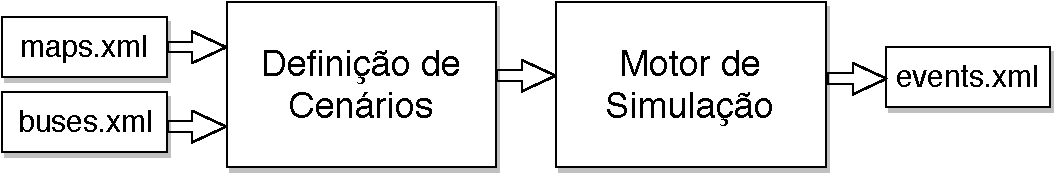
\includegraphics[width=\textwidth]{../figuras/arquitetura-simulador.pdf}
  \caption[Componentes do InterSCSimulator]{Componentes do InterSCSimulator. \label{fig:interscsimulator}}
\end{figure}

  O simulador utiliza dois arquivos principais de entrada para definição do
cenário, são eles map.xml e trips.xml. O primeiro contém a descrição da rede
rodoviária da cidade e é construído com dados obtidos de serviços como Open
Street Maps (OSM)\footnote{\rurl{openstreetmap.org}}. O arquivo é composto por
nós e links, que representam cruzamentos e ruas, respectivamente. A Listagem
\ref{map.xml} mostra um exemplo de um arquivo map.xml com 3 nós e 3 links. Um
usuário da simulação pode ainda fazer alterações nesse arquivo para alterar o
mapa da cidade para atender a um novo cenário, como por exemplo, remover os nós
e links de uma rua conhecida para simular o bloqueio causado por um acidente.
Utilizaremos desse mecanismo para estudar diferentes cenários do trânsito.

\begin{lstlisting}[style=myxml, caption={Exemplo de arquivo map.xml que define a rede rodoviária da cidade. Fonte: \citet{mabs2017}}, label=map.xml]
<network>
  <nodes>
   <node id ="1" x="-46.65805" y="-23.58162"/>
   <node id ="2" x="-46.65828" y="-23.58342"/>
   <node id ="3" x="-46.65228" y="-23.59341"/>
  </nodes>
  <links>
    <link id="35985" from="1" to="2" length="100" free speed="40"/>
    <link id="35985" from="2" to="3" length="200" free speed="40"/>
    <link id="35985" from="3" to="1" length="80"  free speed="50"/>
  </links>
</network>
\end{lstlisting}

  O segundo arquivo de entrada, \emph{trips.xml}, descreve todas as viagens que
devem ser simuladas. Cada viagem deve informar os nós de origem e destino e o
horário da simulação em que ela será iniciada, como pode ser visto na Listagem
\ref{trips.xml}. O caminho entre a origem e o destino pode ainda ser fixada
previamente nesse arquivo ou pode ser calculado pelo simulador, o qual fica
responsável por determinar a rota a ser seguida. Um aspecto interessante é que
se quisermos duplicar o tamanho da simulação, podemos fazer isso simplesmente
duplicando as linhas desse arquivo.

\begin{lstlisting}[style=myxml, caption={Exemplo de arquivo trips.xml que define a rede rodoviária da cidade. Fonte: \citet{mabs2017}}, label=trips.xml]

<scsimulator_matrix>
  <trip origin="247951669" destination="60641382"
    type="car" start_time="28801"/>
  <trip origin="60641382" destination="247951669"
    type="car" start_time="63001"/>
  <trip origin="4511105625" destination="2109902387"
    type="car" start_time="16201"/>
  <trip origin="247951669" destination="60641382"
    type="car" start_time="54001"/>
  <trip origin="246650787" destination="247951670"
    type="car" start_time="54001"/>
  <trip origin="247951670" destination="246650787"
    type="car" start_time="66601"/>
  <trip origin="246650787" destination="60641382"
    type="bus" start_time="54001"/>
</scsimulator_matrix>
\end{lstlisting}

  Cada veículo (carro ou ônibus) definido no arquivo \emph{trips.xml} é um
elemento independente dentro da simulação. Eles percorrem seu trajeto do nó de
origem até o nó de destino seguindo a rede rodoviária da cidade definida no
arquivo \emph{map.xml}.  Cada veículo possui quatro estados dentro da
simulação: \emph{Start}, quando o tempo da simulação atinge o tempo de início
do veículo; \emph{Move}, quando a simulação atinge o tempo do próximo movimento
do veículo; \emph{Wait}, quando o veículo tem que esperar até o próximo
movimento; e \emph{Finish}, quando o veículo chega ao seu destino. Os estados
representam eventos ocorridos dentro da simulação, que são registrados no
arquivo de saída \emph{events.xml}. A Listagem \ref{events.xml} mostra parte de
um arquivo de saída gerado durante uma simulação. É possível ver os eventos de
\emph{start\_trip}, \emph{move} e \emph{finish\_trip} para dois veículos com os
identificadores $2121$ e $2223$.  É importante notar também o atributo
\emph{time}, que indica o tempo de ocorrência do evento dentro da simulação.
Esse atributo  é contabilizado em segundos. Na simulação de um dia do trânsito,
por exemplo, temos então 86400 segundos, correspondentes às 24 horas do dia.

\begin{lstlisting}[style=myxml, caption={Exemplo de arquivo de saída events.xml com os eventos da simulação. Fonte: \citet{mabs2017}}, label=events.xml]

<events version="1.0">
  <event time="4" type="start_trip" vehicle="2121" link="5243" />
  <event time="4" type="start_trip" vehicle="2223" link="1002" />
  <event time="11" type="move" vehicle="2223" link="4005" />
  <event time="31" type="move" vehicle="2121" link="4005" />
  <event time="38" type="move" vehicle="2223" link="2007" />
  <event time="52" type="finish_trip" vehicle="2121" link="4005" />
  <event time="52" type="finish_trip" vehicle="2223" link="5243" />
</events>
\end{lstlisting}

  A partir desse arquivo de saída e do mapa da cidade é possível montar o o
rastro de mobilidade dos veículos ao longo do tempo, recuperando as posições de
latitude e longitude dos \emph{links} sobre o qual eles se movimentam, como
mostra a Tabela \ref{table:rastro}. O rastro de um veículo da simulação pode
ser visto na Figura \ref{fig:rastro}. O ponto verde indica a origem na cor
preta está marcado o destino. Já os pontos vermelhos marcam cada evento de
movimentação que ele fez dentro da simulação.

\begin{table}[!htb]
\centering
\begin{tabular}{|c|c|c|c|c|}
\hline
\textbf{Horário} & \textbf{Ação} & \textbf{ID} & \textbf{Latitude} & \textbf{Longitude} \\
\hline
25 & start & 4858\_52 & -23.624235 & -46.648388 \\
27 & start & 4858\_73 & -23.624235 & -46.648388 \\
27 & start & 94\_17 & -23.535976 & -46.63561    \\
31 & move & 4858\_52 & -23.624077 & -46.648453 \\
33 & move & 4858\_73 & -23.624077 & -46.648453 \\
35 & start & 8394\_43 & -23.561275 & -46.695423 \\
\hline
\end{tabular}
\caption{Tabela com o rastro do tráfego montado a partir do arquivo de saída e o mapa da cidade. \label{table:rastro}}
\end{table}

\begin{figure}[!htb]
  \centering
  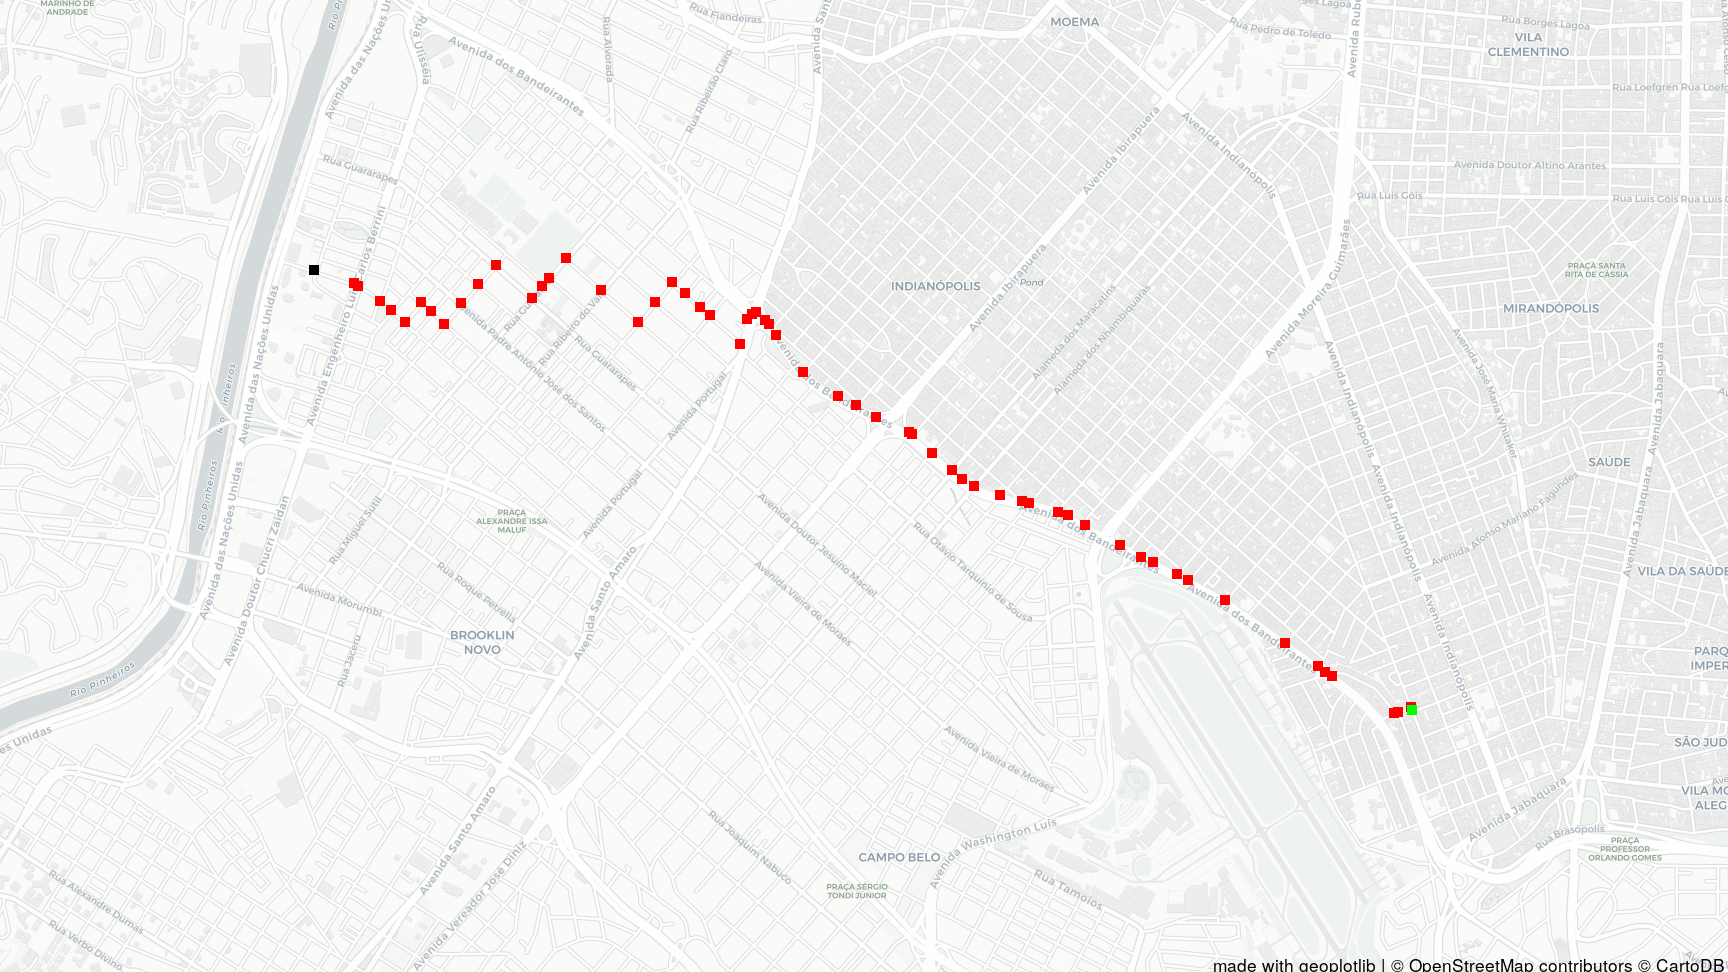
\includegraphics[width=\textwidth]{../figuras/pontos.png}
  \caption{Visualização dos pontos da trajetória do veículo com ID 4858\_52. \label{fig:rastro}}
\end{figure}

Já a Figura \ref{fig:simulated-traffic} mostra uma simples visualização em linhas
de um conjunto de trajetórias do tráfego simulado. Os dados são resultado
da pesquisa de \citet{santana2018courb}, que criaram uma simulação com milhares
de veículos e disponibilizaram os arquivos com os resultados. Utilizamos dados
no intervalo de 1 hora do trânsito filtrando pontos que estivessem entre os
intervalos de tempo $21600$ e $25200$, o que corresponde ao horário entre 6 e 7
da manhã. Note que há bastante oclusão, sendo também impossível distinguir
quais origens vão para quais destinos ou a quantidade de veículos nas vias.

\begin{figure}[!htb]
  \centering
  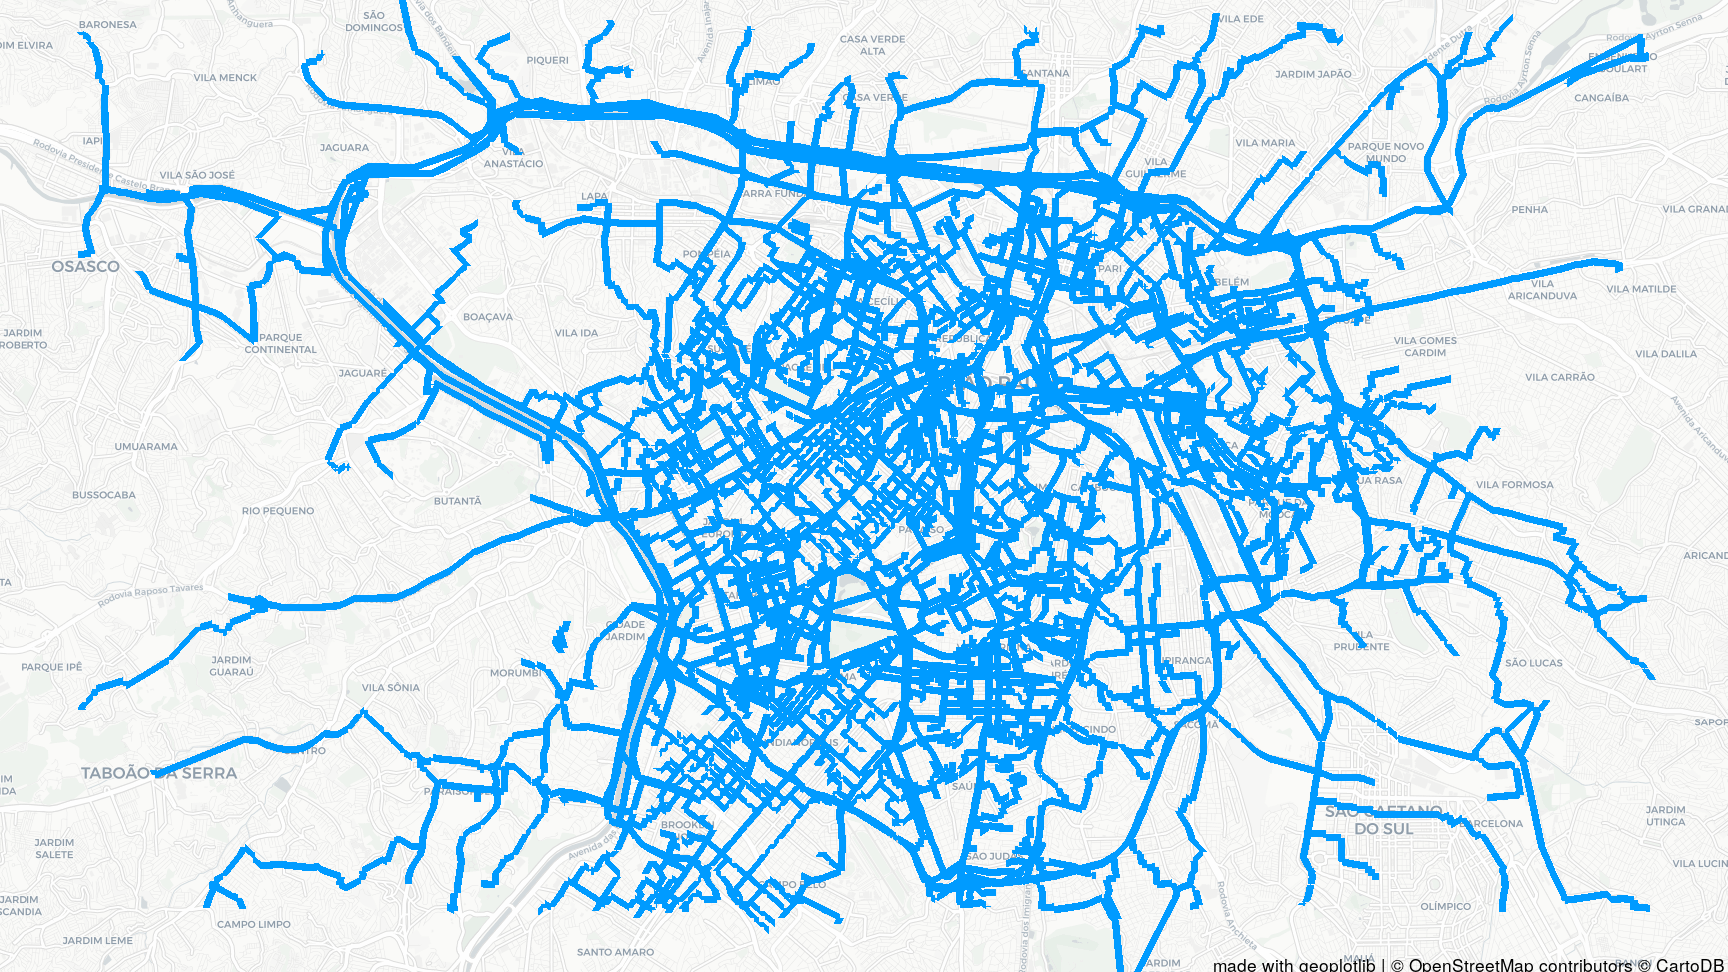
\includegraphics[width=1\textwidth]{../figuras/trafego-ocluso.png}
  \caption{Simulação do tráfego entre 6 e 7 da manhã.}
  \label{fig:simulated-traffic}
\end{figure}

  Os conceitos apresentados servem de base para a nossa proposta de
visualização dos dados do tráfego de veículos no trânsito. O processo processo
de formulação da proposta inclui a definição do tipo de visualização que iremos
utilizar, obter domínio sobre os dados do trânsito e suas propriedades, para
posteriormente chegarmos a uma análise dos fluxos de origem e destino em
diferentes níveis de detalhe a partir de um modelo de \emph{bundling}, além de
investigar formas de destacar essas propriedades dentro da visualização. No
próximo capítulo apresentamos alguns trabalhos que utilizam \emph{bundling} e
outras técnicas para análise de dados de tráfego.

\par
%Falar de visualizações no geral, multi atributos, multi-escalas, agrupamento,
%filtros, cores, bundling, modelos, KDEEB, CUBU.

\chapter{Trabalhos Relacionados}
\label{cap:trabalhos-relacionados}

  A visualização de dados de tráfego tem um amplo histórico. Nossa revisão traz
alguns dos trabalhos e avanços recentes nessa área. As pesquisas que julgamos
relevantes tocam as áreas de visualização da informação - \emph{InfoViz}, cujo
foco é desvendar novos métodos para visualizar uma informação, como
\emph{bundling}, e também a área de análise visual aplicada - \emph{Visual
Analytics}, que se relaciona mais a sistemas e soluções utilizadas em ambientes
do mundo real. Ambos trabalhos trazem contribuições em diferentes níveis para a
nossa pesquisa. Grande parte do conhecimento em visualização do tráfego e
também sobre \emph{bundling} foi consolidado em quatro trabalhos recentes que
fizeram um levantamento geral sobre os esforços na área, os quais apresentamos
\emph{a priori} para depois abordarmos outros trabalhos relacionados à esta
pesquisa.

  \citet{Telea2018} apresenta uma revisão geral das áreas de visualização
científica e de processamento de imagem, apontando métodos utilizados nessas
áreas para que beneficiaram a visualização de grandes grafos multivariados e
complexos. Os novos métodos para simplificação de dados, então chamados de
baseados em imagem, geraram novas técnicas de \emph{bundling} escaláveis, que
permitiram a visualização de grandes grafos, com diversos atributos e
milhares de nós. O algoritmo \emph{Attributed-Driven Edge Bundling} (ADEB), que utilizaremos,
é um dos algoritmos que vêm dessa linhagem e se beneficia desses métodos.

  \citet{Lhuillier2017} traz um estudo ainda mais aprofundado sobre o
\emph{bundling}. Os autores sugerem uma definição formal sobre a operação de
\emph{bundling} em um conjunto de dados, e a partir daí listam as
características, objetivos e limitações de uso das várias técnicas e algoritmos
existentes na literatura. O resultado é uma visão geral sobre o estado da arte
na área e seu desenvolvimento em vários segmentos como grafos, mapas de fluxo,
coordenadas paralelas e outras aplicações. Dentre suas contribuições está uma
nova taxonomia para a ajudar pesquisadores e usuários a selecionarem os
algoritmos de \emph{bundling} com base no tipo de dado.  Apresentamos essa
taxonomia na Figura \ref{table:bundling-methods} na Seção
\ref{sec:modelos-de-bundling}. A partir dela, selecionamos o algoritmo ADEB
para a nossa pesquisa.

  Já \citet{Andrienko2017Visual} e \citet{Chen2015} avaliam uma série de outros
trabalhos que fazem análises de dados do tráfego e de mobilidade em geral e
discutem questões sobre os tipos de dados, técnicas de visualização utilizadas
e principalmente o objetivo das propostas. Os trabalhos listados abrangem
vários contextos, como análise de incidentes no tráfego, monitoramento de
veículos em tempo real, detecção de congestionamentos, sugestão de rotas e
outras atividades executadas por usuários e especialistas de transporte.
Obtemos com estes trabalhos muitos insumos para complementar o conhecimento
sobre a área de visualização e análise de dados de transporte em geral e
enriquecer nossa revisão da literatura. Pudemos utilizá-los como referência
para parte dos conceitos teóricos apresentados na Seção \ref{sec:viz-trafego} e
também como ponte para outras pesquisas na área.

  Além dos estudos citados anteriormente, reunimos um conjunto de trabalhos
cujo o foco está na análise de fluxos de origem-destino em dados do tráfego
para visualização de tendências, fluxos dominantes e seus atributos, como
direção, velocidade, distâncias percorridas e outros.  \citet{Zeng2013} e
\citet{Andrienko2017}  apresentam sistemas interativos para a visualização de
fluxos de origem e destino em dados geoespaciais gerais, logo se encaixam nesse
grupo. Eles propõem novos tipos de leiaute radial para visualizar o tráfego, e
codificam a direção, intensidade e distância percorrida pelos objetos que se
locomovem. \citet{Zeng2013} menciona o uso de \emph{bundling} para agrupar as
linhas dentro do anel de seu leiaute radial (Figura
\ref{fig:interchange-circo}), mas não se aprofundam no assunto.

 \citet{Landersberg2016} usa uma representação em linhas do tráfego sobre um
mapa e apresenta algoritmos de clusterização para agrupar o tráfego por regiões
e também no tempo, reduzindo a oclusão do desenho. Sua análise é focada em destacar diferentes momentos onde há
mudanças significativas nos fluxos. O desafio de sua técnica é estabelecer métricas
que capturam esses momentos.  Eles apresentam um sistema interativo e
verificam seu método com dados de \emph{tweets} geolocalizados na cidade de Londres e
também de redes de celulares. \citet{Klein2014} faz uma análise do tráfego aéreo
da França para detectar as conexões entre os diferentes aeroportos, pontos de
congestionamentos e permitir uma exploração com base em vários atributos, como
direção e altitude dos voos, além de uma janela de tempo que permite navegar
entre diferentes instantes do tráfego. Eles utilizam o algoritmo de
\emph{bundling} KDEEB para reduzir a oclusão na visualização das trajetórias
e apresentam uma interpolação das trajetórias sem \emph{bundling} para visualizar
sua direção, já que o KDEEB não inclui atributos como direção no processo de \emph{bundling}.

\citet{Ferreira2013} fazem uma análise de origem e destino de 500 mil viagens
de táxi feitas em um dia na cidade de Nova Iorque. Sua visualização é baseada
em pontos que destacam as origens e destinos das viagens com cores diferentes.
O resultado é similar a um mapa de densidades que mostra a distribuição das
viagens sobre a cidade. Eles também implementam uma estratégia robusta de
organização dos dados na memória para permitir que os usuários façam buscas e
apliquem filtros em uma grande quantidade de dados de maneira interativa.
\citet{Chu2014} também faz uma análise das trajetórias de milhares de viagens
de táxi em uma grande cidade na China para descobrir relações entre as rotas
utilizadas e relações entre ruas. Eles fazem uma transformação das latitudes e
longitudes para o nome das ruas por onde os taxis trafegam e aplicam métodos de
clusterização e análise de texto que dão uma visão semântica das relações entre
as vias que compõe a malha rodoviária da cidade. Os resultados são mostrados em
um painel com vários tipos de visualização que utiliza mapas, gráficos e outros
recursos para exploração dos dados. \citet{Guo2011} criaram um sistema chamado
TripVista que mostra o tráfego em três perspectivas através de um painel
iterativo.  Seu sistema é focado em mostrar detalhes em nível microscópico
sobre o tráfego em cruzamentos entre ruas da cidade, como direção, quantidade
de veículos e também anomalias de motoristas que trafegam na direção contrária
da permitida. Nos inspiramos nos resultados desse trabalho para investigar como
podemos obter um maior nível detalhes em nossa visualização multiescala com
\emph{bundling}.

\citet{Anita2017} apresenta uma técnica de \emph{bundling}, resultado de uma
otimização do algoritmo FDEB, criado por \citet{Selassie2011}. Para isso,
utilizam uma etapa de clusterização aplicada previamente nos dados, e
posteriormente aplicam o \emph{bundling} em cada cluster. Eles testaram sua
abordagem em vários conjuntos de dados com informações da migração de pessoas
entre regiões dos EUA, migração de pássaros e viagens de aviões, mostrando um
ganho entre 30\% até 50\% no desempenho do algoritmo. A vantagem da sua
abordagem é que ela pode ser utilizada em conjunto com outros métodos de
\emph{bundling}. \citet{Kim2018} utilizam o que eles chamam de \emph{campos
gravitacionais} para construir um mapa de fluxo de dados geoespaciais
analisando apenas as informações estatísticas da distribuições dos pontos ao
longo do tempo. Sua abordagem, no entanto implica uma série de restrições
estatísticas nos dados, como número mínimo de amostras e distribuição uniforme
dos dados ao longo do tempo.

  Em nossa revisão, buscamos obter um panorama geral das lacunas que podem ser
preenchidas em relação ao uso de \emph{bundling} na visualização multiescala
das relações de origem-destino entre regiões da cidade com dados do tráfego de
veículos no trânsito. Observamos vários aspectos de cada trabalho, como o uso
de recursos para visualização de padrões globais e locais do tráfego, o tipo de
objeto do tráfego analisado e tamanho do conjunto de dados, atentando-nos com
interesse especial para fontes de dados do trânsito e também o uso de
\emph{bundling}. Concluímos que as formas de visualizar os dados de trânsito
utilizando técnicas de \emph{bundling} ainda possuem pontos a ser explorados. A
Tabela \ref{table:trabalhos} mostra, em ordem cronológica, os trabalhos que
avaliamos quanto ao uso de dados do trânsito, \emph{bundling} e o leiaute da
visualização.

\begin{table}[htb!]
\begin{tabular}{|M{0.58}|M{0.11}|M{0.115}|M{0.09}|}
\hline
\textbf{Trabalho}       & \textbf{Dados do Trânsito} & \textbf{\emph{Bundling}} & \textbf{Leiaute}  \\ \hline
Nossa proposta          & \checkmark                 & \checkmark               &          linhas   \\ \hline
\citet{Kim2018}         & x                          &  x                       &          linhas   \\ \hline
\citet{Andrienko2017}   & \checkmark                 &  x                       &          radial   \\ \hline
\citet{Anita2017}       & x                          & \checkmark               &          linhas   \\ \hline
\citet{Landersberg2016} & x                          &  x                       &          linhas   \\ \hline
\citet{Klein2014}       & x                          & \checkmark               &          linhas   \\ \hline
\citet{Chu2014}         & x                          &  x                       &          variado  \\ \hline
\citet{Ferreira2013}    & \checkmark                 &  x                       &          pontos   \\ \hline
\citet{Zeng2013}        & x                          & \checkmark               &          radial   \\ \hline
\citet{Guo2011}         & \checkmark                 &  x                       &          variado  \\ \hline

\end{tabular}
\caption[Análise dos trabalhos relacionados]{Análise dos trabalhos relacionados quanto ao uso de dados do trânsito, uso de \emph{bundling} e leiaute da visualização. \label{table:trabalhos}}
\end{table}

  Diferente dos trabalhos apresentados nesta seção, nossa abordagem irá
permitir a análise dos fluxos de origem-destino nas vias de uma cidade.
Propomos o uso de \emph{bundling} para identificar os padrões de movimentação
no trânsito na escala de grandes regiões da cidade e também em escala
microscópica, como em \citet{Guo2011}.  Além disso, os trabalhos relacionados
que utilizam dados de trânsito, como \citet{Andrienko2017, Ferreira2013,
Guo2011}, apresentam visualizações diferentes do leiaute em linhas que
propomos. Contribuímos também com uma análise singular do trânsito na cidade de
São Paulo, onde comparamos com nossa visualização o comportamento do tráfego
com dados reais e dados simulados, o que pode gerar resultados tanto para a
área de visualização quanto para a área de simulação do tráfego. No próximo
capítulo apresentamos a metodologia para o desenvolvimento de nossa proposta
para visualização dos fluxos de origem-destino no tráfego utilizando
\emph{bundling}.

\par

\chapter{Mobilidade em São Paulo}
\label{cap:mobilidade-rmsp}

Para fornecer uma melhor compreensão do cenário de nossa análise, esta seção
descreve as características da Região Metropolitana de S\~ao Paulo e os dados da
última pesquisa OD realizada na região. Para evitar antagonismos entre a
Região Metropolitana de S\~ao Paulo Área (RMSP) e a cidade de S\~ao Paulo, vamos nos
referir à cidade como capital ou simplesmente S\~ao Paulo e vamos nos referir à
área metropolitana como RMSP ou simplesmente área metropolitana. 

\section{Região Metropolitana de São Paulo}

O estado de S\~ao Paulo está localizado no litoral sudeste do Brasil. A Regi\~ao
Metropolitana de S\~ao Paulo é a região mais populosa da América do Sul. De acordo
com o Instituto Brasileiro de Geografia e Estatística \citep{ibge2020}, a RMSP contabilizou $21,9$
milhões de cidadãos em 2020, o que representa cerca de 10\% da população
brasileira. A RMSP é composta por 39 municípios em uma área de \num{7946.84} $km^{2}$. A
cidade de São Paulo é a capital do estado de São Paulo e está localizada no
centro da região metropolitana. A Figura \ref{fig:map-spma} mostra os 39 municípios que compõem a
RMSP. A capital é a cidade mais populosa do Brasil, com 12.3 milhões de
habitantes. Na RMSP, as outras cidades com mais habitantes são Guarulhos (1.4
milhão), São Bernardo do Campo (844 mil), Santo André (721 mil) e Osasco (699
mil).

\begin{figure}[!htb]
  \centering
  \captionsetup{justification=centering}
  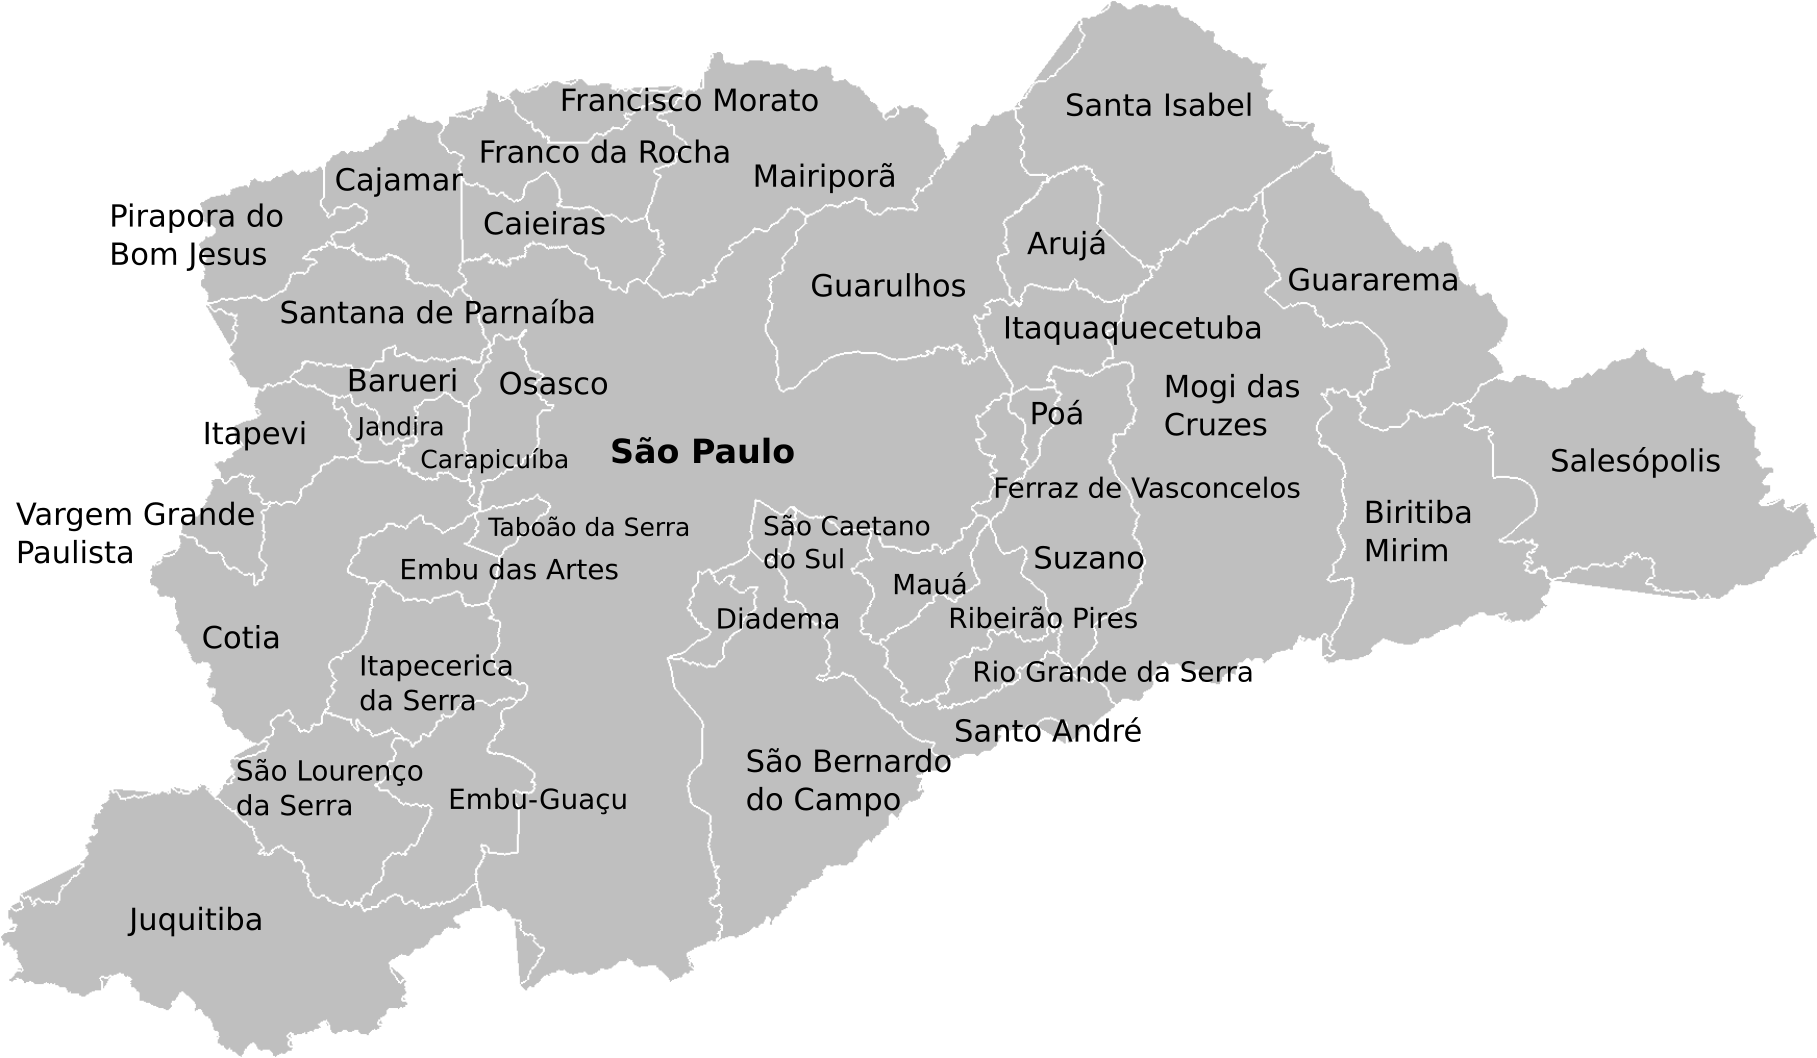
\includegraphics[width=0.95\textwidth]{../figuras/map-spma.png}
    \caption{Municípios da RMSP.\label{fig:map-spma}}
\end{figure}

A capital e as cidades mais próximas concentram a maior parte das oportunidades
de emprego, instalações e serviços públicos, universidades, museus e opções
de entretenimento. Portanto, há um grande deslocamento diário para o centro da
capital e seus arredores. Em São Paulo, os bairros próximos ao centro da
cidade são mais valorizados, portanto, morar nessas partes da cidade tem um maior custo.
Pessoas com menos condições financeiras costumam residir na periferia da capital
ou em outras cidades da RMSP, por isso, algumas cidades da RMSP tornaram-se cidades
dormitório para aqueles que não podem pagar comprar ou alugar uma casa na
capital.

Em relação à infraestrutura de transporte, a capital possui uma rede metroviária
que atende as regiões norte, sul, leste, oeste, sudoeste e sudeste da cidade.
Existem algumas linhas de metrô, a maioria delas cruzando o centro da capital, o
que limita o acesso ao sistema de metrô a algumas regiões da cidade. As demais
cidades não possuem sistemas de metrô, mas existe um outro sistema ferroviário
metropolitano que atende várias cidades do entorno e que é integrado ao sistema
metroviário da capital.

Cada cidade tem seu próprio sistema de ônibus e há um sistema de ônibus
intermunicipal para ligar o cidades vizinhas. Durante o século 20 até o final da
década de 1990, a maioria dos investimentos no transporte foram guiados por uma
abordagem focada no transporte individual de carros em detrimento do transporte
público \cite{rolnik2011}. Os objetivos eram ampliar estradas e ruas para
atender à crescente demanda por carros particulares. Nas últimas duas décadas,
os governos locais têm investido mais em políticas de incentivo ao transporte
público, como implantação de corredores de ônibus e substituição da frota de
ônibus, construção de novas linhas de metrô e modernização do sistema
ferroviário. Além disso, há uma crescente infraestrutura de ciclismo na capital
que vem sendo expandida na última década. Embora esses investimentos tenham
aumentado nos últimos anos, a RMSP ainda sofre com o congestionamento do
tráfego, principalmente nos horários de pico \cite{rolnik2011,ricardo:18}.
Assim, é necessário um melhor entendimento do o comportamento do trânsito na
RMSP para propor novas políticas de melhoria da mobilidade para seus cidadãos.



\section{Pesquisa Origem-Destino}
\label{sec:pesquisa-od}

A pesquisa Origem-Destino (OD) é a principal fonte de informações de mobilidade
sobre a RMSP. Ela é realizada pela Companhia Metropolitana de São Paulo (Metrô) a cada
dez anos, tendo a primeira aplicação em 1967. A última pesquisa OD de 2017 (OD17) tem informações sobre
\num{157992} viagens de pessoas registradas aleatoriamente na RMSP. Os dados representam
uma ampla amostragem da população total e possuem resultados sólidos com uma pequena
margem de erro de 6\% e intervalo de confiança de 92\% \cite[p.18]{odmanual:17}. As viagens ocorrem por diferentes motivos, como
trabalho, casa, estudo e lazer e diferentes modos de viagem, como caminhada,
carro, metrô e trem. Figura~\ref{fig:reason_mode} mostra a distribuição das viagens por meio de
transporte e por motivação. Figura~\ref{fig:trips_by_hour} mostra a distribuição das viagens pelas
horas do dia.

\begin{figure}[ht]
\captionsetup[subfigure]{justification=centering}
\subcaptionbox{Modo de transporte\label{fig:travel-mode}}[0.49\linewidth][l]{%
\begin{tikzpicture}
  \begin{axis}[
    width=.4\columnwidth,
    height=11.5\baselineskip,
    xbar=0pt,
    bar width=8pt,
    bar shift = 0pt,
%    ytick = data,
    y axis line style = { opacity = 0 },
    tickwidth         = 0pt,
    enlarge y limits  = 0.08,
    enlarge x limits  = 0,
    symbolic y coords = {Táxi,Outros,Aplicativo,Bicicleta,Motocicleta,Trem,Ônibus Escolar,Metrô,Passageiro de Carro,Motorista de Carro,Ônibus,Pedestre},
    ytick distance=1,
    xlabel near ticks,
    xlabel={Viagens (x 1000)},
    xmin=0,
    xmajorgrids,
    label style={font=\small},
    tick label style={font=\scriptsize},
    nodes near coords,
    every node near coord/.append style={font=\scriptsize,color=black},
    legend style={at={(0.9,0.2)},anchor=north,legend columns=-1,font=\scriptsize,draw=none},
  ]
  \addplot[fill=blue!80] coordinates {(100.34,Táxi)(111.72,Outros)(368.10,Aplicativo)(376.97,Bicicleta)(1064.11,Motocicleta)(1245.63,Trem)(2093.54,Ônibus Escolar)(3398.96,Metrô)(3529.72,Passageiro de Carro)(7811.67,Motorista de Carro)(8556,Ônibus)};
  \addplot[fill=blue!80, every node near coord/.append style={xshift=-4em,font=\scriptsize,color=white},] coordinates {(13349.88,Pedestre)};
    \legend{Viagens}
  \end{axis}
\end{tikzpicture}
}%
\subcaptionbox{Motivo da viagem\label{fig:travel-reason}}[0.49\linewidth][r]{%
\begin{tikzpicture}
  \begin{axis}[
    width=.4\columnwidth,
    height=11.5\baselineskip,
    xbar=0pt,
    bar width=8pt,
    bar shift = 0pt,
%    ytick = data,
    y axis line style = { opacity = 0 },
    tickwidth         = 0pt,
    enlarge y limits  = 0.08,
    enlarge x limits  = 0,
    symbolic y coords = {Busca por emprego,Alimentação,Lazer,Saúde,Shopping,Assuntos pessoais,Escola,Trabalho,Casa},
    ytick distance=1,
    xlabel near ticks,
    xlabel={Viagens (x 1000)},
    xmin=0,
    xmajorgrids,
    label style={font=\small},
    tick label style={font=\scriptsize},
    nodes near coords,
    every node near coord/.append style={font=\scriptsize,color=black},
    legend style={at={(0.9,0.2)},anchor=north,legend columns=-1,font=\scriptsize,draw=none},
  ]
  \addplot[fill=blue!80] coordinates {(95.01,Busca por emprego)(560.46,Alimentação)(960.01,Lazer)(968.33,Saúde)(1019.91,Shopping)(1370.02,Assuntos pessoais)(7648.32,Escola)(9987.14,Trabalho)};
  \addplot[fill=blue!80, every node near coord/.append style={xshift=-4em,font=\scriptsize,color=white},] coordinates {(19397.47,Casa)};
  \legend{Viagens}
  \end{axis}
\end{tikzpicture}
}%
\caption{Registros por modo de transporte e por motivo da viagem.}
\label{fig:reason_mode}
\end{figure}

\begin{figure}
\begin{tikzpicture}
  \begin{axis}[
    ybar=0pt,
    bar width=8pt,
    bar shift = 0pt,
    width=\textwidth,
    height=0.5\textwidth,
    tickwidth         = 0pt,
    enlarge y limits  = 0,
    enlarge x limits  = 0.05,
    symbolic x coords = {0h,1h,2h,3h,4h,5h,6h,7h,8h,9h,10h,11h,12h,13h,14h,15h,16h,17h,18h,19h,20h,21h,22h,23h},
    xtick = data,
    ylabel near ticks,
    ylabel={Viagens (x 1000)},
    xlabel={Hora},
    ymin=0,
    ymajorgrids,
    y axis line style = { opacity = 0 },
    label style={font=\small},
    tick label style={font=\scriptsize},
    nodes near coords,
    every node near coord/.append style={font=\scriptsize,color=black,yshift=0.05cm,rotate=90,anchor=west,inner sep=0.3pt},
    legend style={at={(0.9,0.95)},anchor=north,legend columns=-1,font=\footnotesize,draw=none},
  ]
  \addplot[fill=blue!80] coordinates {(0h,110.43)(1h,46.91)(2h,40.71)(3h,27.19)(4h,409.84)(5h,1044.41)(6h,4619.43)(7h,3637.29)(8h,1775.78)(9h,1221.95)(10h,1207.14)(11h,2074.15)(12h,5245.01)(13h,2674.60)(14h,1581.01)(15h,1413.75)(16h,2264.21)(17h,4100.44)(18h,4084.74)(19h,1409.82)(20h,763.59)(21h,590.73)(22h,1194.25)(23h,469.26)};
  \legend{Viagens}
  \end{axis}
\end{tikzpicture}
\caption{Viagens por hora do dia.}
\label{fig:trips_by_hour}
\end{figure}

Como mostra a Figura~\ref{fig:reason_mode}, a maioria das viagens na cidade são feitas por
pedestres. Normalmente, viagens de pedestres cobrem pequenas distâncias (624m em média)
e ficam dentro de um único distrito da cidade. Podemos perceber também que há
um número significativo de viagens de carro e de transporte público
(ônibus, metrô e trem), a maioria mais longa (7,7 km em média), principalmente
de trem e metrô (13,5 km em média). Olhando para viagens por hora (Figura~\ref{fig:trips_by_hour}),
é possível notar que o trânsito na RMSP tem três picos principais: pela manhã (6h às 8h),
na hora do almoço (meio-dia) e no início da noite (17h às 19h).

Os \num{157992} registros da pesquisa OD possuem inúmeros atributos sobre as
viagens. Os mais relevantes para nosso estudo, no entanto, são as coordenadas de
origem e destino (quantitativo) e o fator de expansão da viagem (quantitativo),
que é a extrapolação estatística para o tamanho da população que cada viagem
pesquisada representa. Ou seja, o fator de expansão somado a todas as entradas
da pesquisa resulta em 42 milhões de viagens em um dia útil típico. Outros
atributos são o horário de saída (quantitativo), o meio de transporte
(categórico, 17 valores: trem, metrô, motorista de carro, passageiro de carro,
ônibus da cidade de São Paulo e de outras cidades, ônibus intermunicipal,
monotrilho, veículo fretado, ônibus escolar, táxi regular, táxi não regular,
motorista de motociclista, passageiro de motociclista, pedestre, bicicleta e
outros) e o motivo da viagem (categórico: trabalho, casa, estudo e lazer).

A Figura~\ref{fig:cluttered-graph} mostra as viagens da pesquisa OD desenhadas sobre o mapa do
RMSP, onde cada linha representa uma trajetória da OD. A extrema oclusão na figura
impede a visualização de trajetórias individuais, padrões de tráfego ou conexões
entre as regiões do mapa. A partir dessa imagem, podemos apenas inferir a
existência de tráfego intenso na maior parte da região metropolitana e uma
concentração significativa desse tráfego no centro de São Paulo. Além disso,
esta imagem não mostra nenhum dos atributos de dados disponíveis, exceto O e D.
Portanto, as técnicas de filtragem e agregação são essenciais para simplificar a
visualização e torná-la compreensível.

\begin{figure}[!htb]
  \centering
  \captionsetup{justification=centering}
  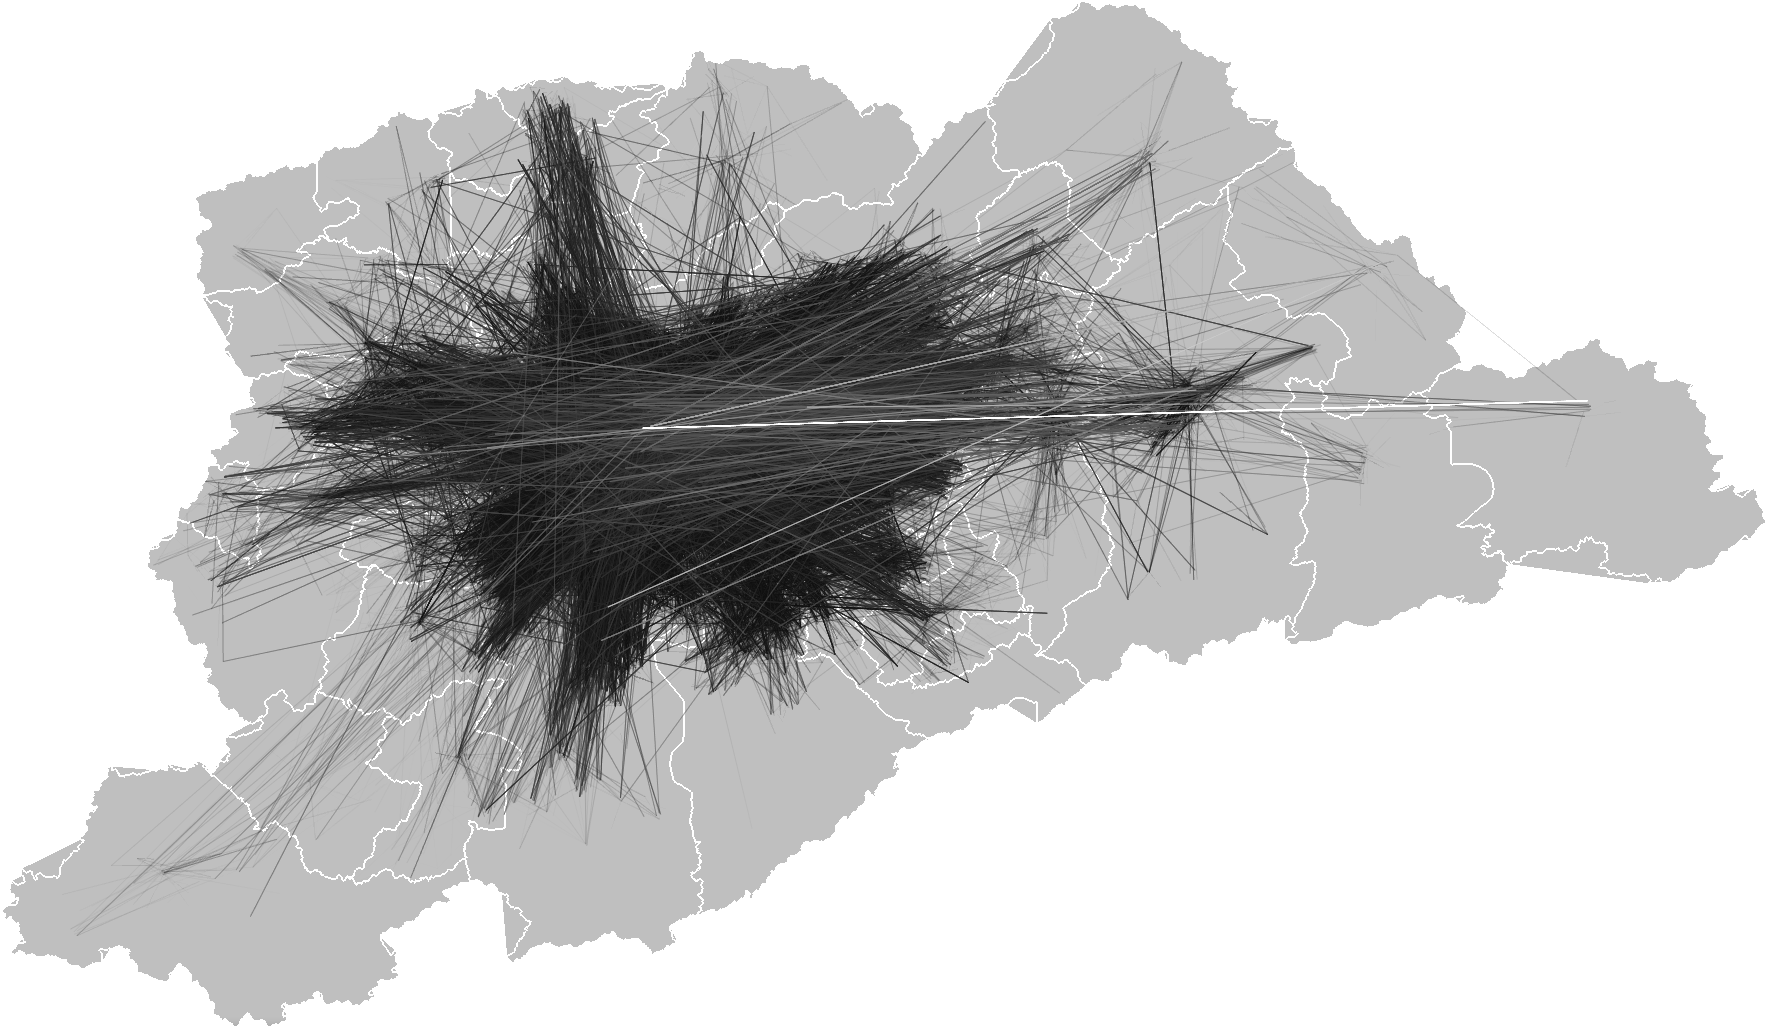
\includegraphics[width=0.95\textwidth]{figuras/unbundled-edges+grayscale+512px.png}
  \caption{Desenho puro das viagens da OD sobre a RMSP.\label{fig:cluttered-graph}}
\end{figure}
\par
%Trabalhos que usam bundling na visualização de dados em geral (outros modelos/frameworks)
%Trabalhos que usam visualização de dados de OD, com bundling ou não
%Trabalhos que usam o CUBU 
%Trabalhos que usam os dados da OD

\chapter{Metodologia}
\label{cap:metodologia}

Para explorar a visualização dos fluxos de mobilidade urbana utilizamos em nosso
estudo dados públicos da pesquisa OD17. Esses dados representam milhões de viagens
que ocorrem diariamente em um dia normal de trabalho na Região Metropolitana
de São Paulo (RMSP). Parametrizamos e adaptamos o \emph{framework} de visualização \emph{CUBu} para explorar várias
propriedades do tráfego com diferentes usos do \emph{bundling}. A seguir
detalhamos cada uma das etapas que seguimos.

\section{Representação dos Dados}

Os dados da pesquisa OD que usamos como entrada para o \emph{bundling} são
descritos por uma tabela com 6 (seis) colunas: ID da viagem, modo de transporte,
horário de partida, horário de chegada, coordenadas de origem e coordenadas de
destino; O ID da viagem é o identificador obtido
diretamente do conjunto de dados da OD17 e representa uma entrada única no conjunto
de dados. O modo de transporte é armazenado como um número inteiro no intervalo
de 1 a 17 e corresponde a cada um dos diferentes modos presentes na pesquisa OD17.
Os horários de partida e chegada são armazenado como um número de ponto
flutuante no intervalo de [0.0 - 23:59]. Por último, temos as coordenadas de
origem e destino, o principal atributo do conjunto de dados. Em se tratando de
coordenadas, diversos sistemas podem ser utilizados; em nossa pesquisa
transformamos todas as coordenadas para o sistema de latitude / longitude para a
correta geo-localização das viagens no mapa, que também utiliza este formato.

Um outro atributo importante é o fator de expansão de cada registro da OD17 (apresentado na Seção~\ref{sec:pesquisa-od}),
o qual é utilizado para extrapolação estatística da quantidade real estimada de viagens.
Desta forma, dado o registro de uma viagem da pesquisa OD17 contendo um fator de expansão $E$, criamos $E$
cópias desse registro para utilizar como entrada da nossa visualização com \emph{bundling}. Isso produz um conjunto de dados completo de 42
milhões de viagens. Para todas essas viagens replicadas, mantemos seu ID original
obtido da pesquisa OD17 que a gerou. Dessa forma, podemos rastrear quais viagens
agrupadas correspondem a um registro da OD17. Além desses dados básicos que apresentamos, atributos
extras da pesquisa OD17 podem ser adicionados, como o motivo da viagem (ver
Seção~\ref{sec:pesquisa-od}) e também dados pessoais (idade, renda). A pesquisa
OD é bastante rica e pode produzir um conjunto de dados com mais de dez atributos por viagem.
A Tabela~\ref{table:data-input} mostra um exemplo das viagens geradas com duas
viagens replicadas a partir de um registro da OD com ID 50 e fator de expansão $E=2$.

% Using the siunitx package to align and round
% numbers (columns of type "S")
\begin{table}[!htb]
  \small
  \newcommand{\hdr}[1]{\bfseries#1}
  \sisetup{
    mode=text,
    round-mode=places,
    round-precision=6,
    table-figures-integer=2,
    table-figures-decimal=6,
    table-number-alignment=left,
    table-text-alignment=left,
    table-space-text-post=nn,
  }
  \centering
  \caption{Formato de dados utilizados como entrada para o \emph{bundling}.\label{table:data-input}}
  \begin{tabular}{>{\footnotesize}l>{\footnotesize}c>{\footnotesize}l>{\footnotesize}l>{\footnotesize}S>{\footnotesize}S>{\footnotesize}S>{\footnotesize}S}
    \toprule
    \multirow{2}[2]{*}{\hdr{ID}} & \multirow{2}[2]{*}{\hdr{Modo}} & \hdr{Saída} & \hdr{Chegada} & \multicolumn{2}{c}{\hdr{Origem}}   & \multicolumn{2}{c}{\hdr{Destino}}\\
     &  & \hdr{hora} & \hdr{hora} & \hdr{Longitude}   & \hdr{Latitude}    & \hdr{Longitude}     & \hdr{Latitude}\\
    \midrule
    50         & 1   & 6.45 & 7.10  & -46.62809376987491 & -23.551691865840347 & -47.00348104352116 & -23.39356328288028\\
    50         & 1   & 6.45 & 7.10  & -46.62809376987491 & -23.551691865840347 & -47.00348104352116 & -23.39356328288028\\
    51         & 4   & 8.30 & 9.05  & -47.00187231236886 & -23.39846860627696  & -47.00348104352116 & -23.39356328288028\\
    \bottomrule
  \end{tabular}
\end{table}

\section{Pré-processamento dos dados}

Como mencionado na Seção~\ref{sec:pesquisa-od}, o conjunto de dados possui \num{157992} viagens,
e que ao considerarmos o fator de expansão, esse número cresce para pouco mais de 42 milhões.
Embora \emph{CUBu} seja - de acordo com seus autores e também com nosso conhecimento - a
solução mais rápida existente para agrupamento com \emph{bundling}, ele ainda não
seria capaz de processar 42 milhões de viagens e responder de maneira rápida para
exploração interativa dos dados. Para lidar com este problema, utilizamos uma abordagem
para reduzir o conjunto de dados OD17 com base no fator de expansão $E$.

Primeiramente, analisamos quão representativos eram os registros amostrais da
OD17 em relação a população total de 42 milhões de viagens. Observamos que todos os
registros com fator de expansão $E < 75$, quando somados, representavam menos de 4\% da população total de 42
milhões. Considerando que a margem de erro da pesquisa OD17 é inferior a 6\%
(ver Seção~\ref{sec:pesquisa-od}), podemos remover os registros com $E < 75$ e
ainda assim manter a representatividade do conjunto de dados. Então, pudemos dividir
os valores $E$ de todos os registros restantes por esse valor limite de 75,
resultando em um número menor de viagens a serem duplicadas, e ainda preservar
a distribuição de dados. No entanto, embora 75 seja um valor dentro de um
limite razoável para aplicar a redução, conforme explicado acima, para minimizar
a perda de dados e evitar grandes alterações nas suas propriedades, nós
utilizamos na prática um limite menos agressivo de 55. A
Figura~\ref{fig:expansion-factor} mostra o percentual acumulado de registros que
são removidos pela escolha de determinados valores do fator de expansão, quanto
maior o valor, mais dados são perdidos na redução. Essa abordagem nos permitiu
reduzir significativamente o número de viagens, de 42 milhões para \num{685115},
o que resultou em menos de 2,5\% de perda de informações.

\begin{figure}
\begin{tikzpicture}
  \begin{axis}[
    ybar=0pt,
    bar width=18pt,
    bar shift = 0pt,
    width=\textwidth,
    height=0.5\textwidth,
    tickwidth         = 0pt,
    enlarge y limits  = 0,
    enlarge x limits  = 0.05,
    symbolic x coords = {5,10,15,20,25,30,35,40,45,50,55,60,65,70},
    xtick = data,
    ylabel near ticks,
    ylabel={Percentual de viagens},
    xlabel={Fator de expansão $E$},
    ymin=0,
    ymajorgrids,
    y axis line style = { opacity = 0 },
    label style={font=\small},
    tick label style={font=\scriptsize},
    nodes near coords,
    every node near coord/.append style={font=\scriptsize,color=black,yshift=0.25cm,rotate=0,anchor=north,inner sep=0.3pt,/pgf/number format/fixed},
    legend style={at={(0.1,1.0)},anchor=north,legend columns=-1,font=\footnotesize,draw=none},
  ]
  \addplot[fill=blue!80] coordinates {(5,0.0052)(10,0.0363)(15,0.1235)(20,0.2258)(25,0.4561)(30,0.6931)(35,0.9593)(40,1.3396)(45,1.6128)(50,2.0119)(55,2.3489)(60,2.7709)(65,3.1686)(70,3.4546)};
  \legend{Viagens ($\%$)}
  \end{axis}
\end{tikzpicture}
\caption{Percentual acumulado da perda de registros em função do fator de expansão.}
\label{fig:expansion-factor}
\end{figure}

\section{Filtragem e particionamento dos dados}

Além do processo de redução de dados explicado acima, também aplicamos dois
outros métodos de simplificação, \emph{filtragem} e \emph{particionamento}. Tais
técnicas permitem um outro olhar para características específicas do conjunto de
dados e funcionam de maneira complementar. Com as duas abordagens,
exploramos duas diferentes utilizações do \emph{bundling}, o que permitiu uma
experiência maior para avaliar o potencial da técnica na análise
de grandes conjuntos de dados de mobilidade urbana com múltiplos atributos.

Para ver as relações entre os diferentes modos de transporte e as direções do
tráfego durante os horários de pico, usamos filtros visuais que tornam as
trajetórias indesejadas totalmente transparentes na visualização. Isso é
particularmente útil quando queremos visualizar relações entre dados diferentes,
por exemplo, para explorar como os ônibus de São Paulo se relacionam com os
ônibus de outras cidades vizinhas. Nesse caso, aplicar \emph{bundling} em todo o
conjunto de dados e, em seguida, diferenciá-los de alguma forma na visualização,
é uma maneira sugestiva de visualizar suas relações. A diferenciação pode ser
feita de várias formas, e aqui utilizamos cores diferentes para cada tipo de
transporte e opções de filtro diferentes, os quais abordaremos adiante.

Para outros tipos de análises, como as relacionadas ao motivo da viagem, renda
familiar e idade dos passageiros, nós particionamos o conjunto de dados em cada
um desses atributos separadamente e aplicamos o \emph{bundling} a esses
subconjuntos. As vantagens dessa abordagem é que ela permite observar cada
atributo com mais detalhes, pois remove a interferência de outros dados, além de
ser mais simples de se executar.

\section{Parâmetros do \emph{bundling}}

Referências da literatura não são claras sobre como escolher bons parâmetros de
\emph{bundling}, \citet{Lhuillier2017}. Isso também foi observado e explicitamente
estudado por \citet{zeng:19}, que também propôs maneiras de calcular boas
configurações de parâmetros. No entanto, como eles também mencionam, essas
configurações são válidas para seu método de \emph{bundling} (RAEB) e não
generalizam diretamente para outros métodos, como o \emph{CUBu}. Portanto,
tivemos que encontrar bons parâmetros para nosso estudo empiricamente. Os
parâmetros obtidos dessa forma foram: resolução da imagem $I = 512 x 512$
pixels; taxa de preenchimento $S = 10$ pixels (de acordo com a recomendação de
\cite{zwan:16} de usar 1\% da diagonal da imagem); raio do \emph{kernel} $k = 18$
pixels; e número de iterações do \emph{bundling} $N = 15$. Em nosso maior
conjunto de dados, representado por todas as \num{685115} viagens, esta
configuração gerou cerca de 3,2 milhões de pontos, que foram agrupados em cerca
de 52 milissegundos por iteração em um PC com uma placa de vídeo NVidia GeForce
940MX de 4 GB. Usamos esse conjunto de parâmetros para criar a maioria das
visualizações agrupadas mostradas a seguir na Seção~\ref{sec:results}, exceto para as da Seção~\ref{sec:classes},
onde mostramos os padrões de deslocamento de diferentes classes sociais.
Para esses subconjuntos específicos, reduzimos a taxa de preenchimento $S$ para
5 pixels e modulamos a transparência $alpha$ do mapa de densidade para 0,15. Na
prática, ao utilizarmos metade do valor de $S$ dobramos o número de pontos na
visualização;  Observamos que as mudanças desse dois parâmetros ajudam a
destacar os pontos de densidade que buscamos em nossa análise sem impacto na
estrutura da visualização.

% TODO arrumar referencias das seções 5 e 5.6 no paragrafo anterior

\section{Melhorias na visualização}

Para enriquecer nossas visualizações da mobilidade urbana de São Paulo, fizemos
algumas importantes adições ao \emph{CUBu}. Primeiro, adicionamos o mapa da área
metropolitana como imagem de fundo e também a possibilidade de desenhar as
linhas de metrô e trem na visualização. Dessa forma, podemos utilizar o mapa
para localizar melhor onde os \emph{bundles} estão posicionados e podemos usar
os trilhos para explorar como os \emph{bundles} se correspondem com a
infraestrutura ferroviária da cidade (ver Seção~\ref{sec:trail-overlap}). Além
disso, implementamos filtros para selecionar subconjuntos dos 17 modos de
transporte a serem exibidos na visualização, usando cores categóricas diferentes
para cada um deles (ver Seção~\ref{sec:coloring} e filtros de tempo para selecionar fluxos de movimentação em
horários específicos do dia (ver Seção~\ref{sec:peak-hours}). Usamos esses recursos para explorar a diferentes
relações entre os fluxos e seu impacto na mobilidade urbana.

\par
%Aqui a gente fala dos dados da OD que vamos utilizar. O que representam, como
%obter, quais vamos usar e porque.
%
%Aqui falamos do framework CUBU, suas funcionalidades, como obtivemos e como
%vamos implementar coisas novas nele


%O que vou mostrar/experimentar: exemplos dentro de algumas categorias
%
%
%1) Explorando as propriedades espaciais (coisas óbvias)
%- Aplicar o bundling para ver regiões densas, conforme mostrados na OD
%	x) Mostrar as features de cores padrão (distância, direção, densidade)
%	x) Mostrar as features de cores implementadas (tipo de transporte, modo de transporte, renda, gênero)
%	x) Mostrar que tem pessoas que andam de metrô em locais que não tem metrõ (adicionar mapa)
%	x) Mostrar como os ônibus metropolitanos se interceptam com os de são paulo
%	x) Mostrar que os filtros de dados por horário pra mostrar que há mais fluxo
%		 no horário de pico, que os onibus escolares saem todos pela manhã, mas que também temos
%		pessoas que saem de madrugada para trabalhar
%	x) Mostrar a renda e correlacionar distância do centro com renda
%	x) Mostrar correlação de renda com carro (pobre anda de carro?)
%
%	- Quais vantagens e desvantagens em relação ao que existe na OD (substitui alguma coisa do relatório da OD?)
%	- Qual o nível de detalhes conseguimos extrair alguma informação?
%
%
%2) Mostrar a mesma grandeza de diferentes maneiras
%- Grandezas: Tempo/Tipo de transporte/Direção
%- Estratégias: Fazer bundle de tudo e aplicando filtro&cores vs separado, diferenciar por cores no bundling de tudo, e filtrar as arestas no tempo (manhã e tarde)
%	x) Fazer bundling de todos os dados de transporte e filtrar por modo
%	x) Fazer bundling de todos os dados de transporte e colorir por modo
%	x) Fazer bundling dos modos de transporte separados
%	x) Fazer bundling dos dados em direção opostas
%	x) Filtrar por horário de pico
%	x) Derivar um atributo do quão o horário de pico afeta e usar como VALUE
%	x) Usar o fator de expansão para mostrar a densidade como VALUE
%
%	Vantagens e desvantagens em relação aos gráficos da OD?
%	Qual os níveis de detalhes conseguimos obter?
%
%
%3) Escalar o agrupamento conforme o zoom e resolução diferentes e dados diferentes (tunning não muito óbvio)
%	- Número de pontos
%	- Resolução da imagem
%	- tamanho do kernel
%	- Glanuralidade dos dados
%	x) Aplicar bundling com alta resolução e alto numero de pontos, kernel grande e kernel pequeno
%	x) Aplicar bundling com alta resolução e baixo numero de pontos, kernel grande e kernel pequeno
%	x) Aplicar bundling com baixa resolução e alto numero de pontos, kernel grande e kernel pequeno
%	x) Agrupar os dados na mão em regiões e aplicar o bundling em macro regiões. Qual a alguma diferença?
%	x) Mostrar o bundling dos dados dos centróides e dos dados específicos em alguns modais (metrô, a pé, bike, taxi)
%
%	Explicar que não há uma métrica, mas dissertar sobre qual fica melhor visualmente
%	- Vantagens e desvantagens em relação às visualizações da OD em diferentes escalas
%
%4) Evolução temporal
%	- Desafios: Correspondência de regiões
%	x) Aplicar bundling de tudo: filtrar por ano
%	x) Aplicar bundling separado em cada ano
%	x) Aplicar bundling na diferença de um ano pro outro
%
%	Que vantagens/diferenças consigo ver em relação aos relatórios da OD?
%	- Falar de bundling estático e dinâmico, mas que é future work...


% \chapter{Resultados}
\label{sec:results}

Essa seção apresenta os resultados das análises que desenvolvemos sobre os dados
da pesquisa OD 17. Começamos com a exploração dos recursos de visualização
oferecidos pelo \emph{CUBu}, com ênfase na codificação visual dos atributos
densidade, distância e direção das viagens. Esses aspectos são apresentados a
seguir nas
Seções~\ref{sec:density},~\ref{sec:trail-overlap},~\ref{sec:length-direction},~e~\ref{sec:coloring}.
Posteriormente, utilizando tais recursos visuais analisamos outros padrões de
mobilidade específicos a subconjuntos dos dados, detalhados nas
Seções~\ref{sec:strata},~\ref{sec:students},~\ref{sec:peak-hours},~\ref{sec:dist_reasons},~e~\ref{sec:mode}.

\section{Visualizando a densidade dos \emph{bundles}}
\label{sec:density}

Na Seção~\ref{sec:bundling}, explicamos como a operação de \emph{bundling}
faz o agrupamento de trajetórias simplificando a visualização e reduzindo a oclusão
da imagem. No entanto, tal operação não nos diz quantas trajetórias foram agrupadas em
um \emph{bundle}. A solução para isso, primeiramente apresentada por \citet{holten06},
é desenhar linhas semi-transparentes, cada uma com uma transparência fixa $\alpha < 1$.
Assim, a combinação mostrará trajetórias de alta densidade como mais opacas e as de baixa
densidade como mais transparentes. Apesar da transparência ajudar na diferenciação
de áreas densas, ela por si só não é uma variável visual quantitativa forte \citep{slocum09}.
Então, codificamos também a densidade das trajetórias em cores, utilizando
os valores estimados pelo KDE durante o processo de \emph{bundling} (ver Seção~\ref{sec:bundling}).
A Figura~\ref{fig:bundled-graph-density}a mostra uma visualização obtida usando codificação
da densidade em cores aplicada em todo o conjunto de dados da OD17 contendo
as \num{685115} viagens. Podemos ver alguns caminhos com maior densidade, mas a imagem
ainda apresenta uma demasiada carga de informação e muitas áreas opacas. Isso ocorre pelo fato de que,
usualmente em GPUS de consumo comum, a transparência $\alpha$ é modelada por um valor
inteiro de 8 bits. Portanto, apenas 255 níveis de transparência diferentes são possíveis,
ou seja, apenas 255 níveis de densidade das trajetórias podem ser exibidos. Valores
de $\alpha$ muito altos saturam o canal de transparência
onde ocorrem as densidades mais altas - todas as densidades acima de 255 são fixadas
em 255. Valores abaixo de 1/255 resultam em nenhuma imagem, uma vez que
isso corresponde a opacidade zero na representação de 8 bits.

Para resolver este problema, mapeamos a densidade $\rho$ de duas maneiras,
transparência e cor. Já que $\rho$ é calculado precisamente como um número
de ponto flutuante durante a estimação do KDE, nenhum valor é truncado ou arredondado.
Essa estimativa da densidade permite modular a transparência para destacar ainda
mais as áreas de alta densidade e reduzir a oclusão da imagem. Uma outra alternativa
seria utilizar valores maiores de \emph{kernel} $k$, o que agruparia ainda mais as trajetórias, gerando
\emph{bundles} mais fortes, porém também iria causar uma maior distorção das linhas.
A Figura~\ref{fig:bundled-graph-density}b mostra o \emph{bundling} aplicado nos mesmos
dados da Figura~\ref{fig:bundled-graph-density}a. Podemos observar que os \emph{bundles}
aparecem mais salientes após aplicar a modulação da transparência. A imagem sugere que a rede do tráfego metropolitano
pode ser dividida em algumas ramificações principais que são fortemente conectadas à área central,
onde a cidade de São Paulo está localizada. Isso faz sentido considerando que esta é a parte
mais populosa da área metropolitana. Além disso, a maioria dos sistemas de transporte
cruzam o centro da capital, incluindo linhas de metrô, trem, e as principais vias expressas.

\begin{figure}[!htb]
  \centering
  \captionsetup{justification=centering}
  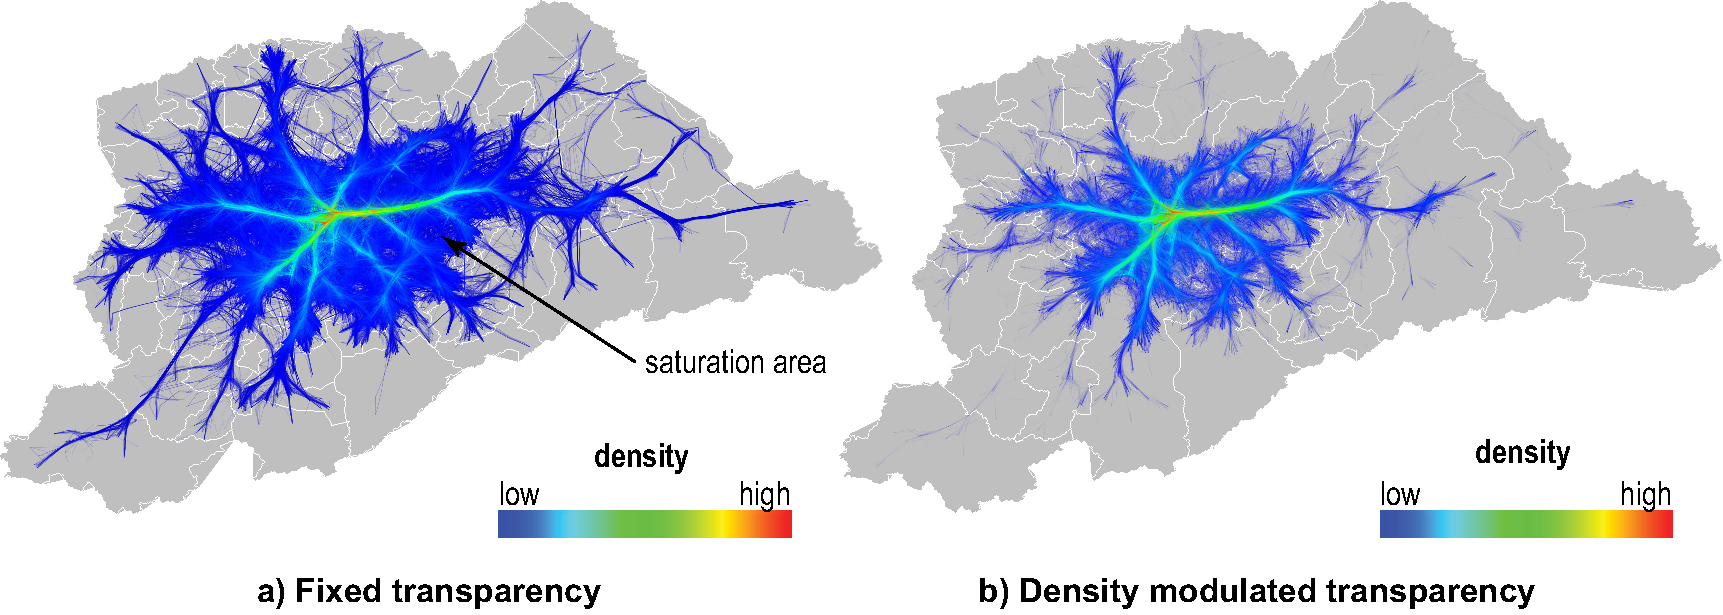
\includegraphics[width=0.98\textwidth]{../figuras/figure1}
  \caption{\emph{Bundling} das trajetórias coloridas pela densidade (a) valores fixos e \\(b) transparência modulada.}
  \label{fig:bundled-graph-density}  
\end{figure}

% % How we calculated 44%:
% %
% % 1. Take all trips that indicate bus, metro, and train as
% %    the main transportation mode -> this is the amount of
% %    trips by public transportation
% %
% % 2. Take all trips that indicate use of metro or train for
% %    some portion of the trip and divide that by the amount
% %    of trips by public transportation
% %
% % Using the tables from pages 46 and 49 of
% % http://www.metro.sp.gov.br/pesquisa-od/arquivos/Ebook%20Pesquisa%20OD%202017_final_240719_versao_4.pdf
% %
% % We consider that:
% % trips using bus as the main transportation mode: 8034
% % trips using train as the main transportation mode: 1245
% % trips using metro as the main transportation mode: 3400
% % total trips by public transportation: 8034 + 1245 + 3400 = 12679
% %
% % trips using metro for some portion of the trip: 3400
% % trips using train for some portion of the trip: 2272
% % total trips involving train or metro: 3400 + 2272 = 5672
% %
% % Percentage = 5672*100/12679 = 44.73%
% %
% % Not relevant for the text, just a curiosity:
% % the percentage in relation to all motorized trips is 5672*100/28280=20.05%

\section{Infraestrutura de metrô e trem \emph{vs.} \emph{bundling}}
\label{sec:trail-overlap}

O sistema de transporte público é o mais utilizado pelos moradores da RMSP. O
impacto da malha ferroviária sobre o deslocamento de pessoas fica claro quando
desenhamos as linhas ferroviárias ao longo das trajetórias agrupadas com o
\emph{bundling}. A Figura~\ref{fig:rails} mostra a alta correspondência dos
\emph{bundles} com os caminhos das linhas ferroviárias (desenhadas em preto).
Tendo em vista que, de acordo com a pesquisa OD17, cerca de 44\% das viagens
diárias de transporte público envolvem metrô ou trens, este é um resultado
esperado. Curiosamente pode-se questionar se o sistema ferroviário foi planejado
com precisão para atender a demanda, como sugere a visualização agrupada, ou se
a disponibilidade dessa opção de transporte influenciou a existência de fluxos
tão densos. Embora não temos os insumos para responder a essa pergunta, os
gestores de tráfego podem usar esse tipo de visualização para elaborar políticas
para o transporte público. Apesar de não expressar nenhuma grande surpresa sobre os
dados analisados, este é um resultado bastante importante, pois consideramos que a alta
correlação entre o \emph{bundling} das trajetórias e as linhas das ferrovias
também indica boas configurações de parâmetros para esse tipo de visualização na
escala da região metropolitana.

Ressaltamos que que este tipo de correlação (de \emph{bundles} com estradas) não
é o mesmo que o utilizado no método RAEB \citep{zeng:19}. No método RAEB, o
agrupamento foi feito explicitamente para seguir estradas. Em nosso caso, as
linhas são sobrepostas sobre \emph{bundles}, que foram gerados unicamente a partir dos
dados da OD. Pode-se argumentar que RAEB, neste sentido, produz \emph{bundles}
mais ``corretos'', uma vez que estes são forçados para seguir as estradas. No
entanto, olhando mais de perto, podemos ver que RAEB não pode ter todos os
\emph{bundles} seguindo precisamente todos os caminhos das estradas - pois isso
basicamente bloquearia qualquer agrupamento do \emph{bundling} e resultaria no próprio
mapa das estradas. Além disso, RAEB requer que o registro dos pontos das trajetórias
seja feito dentro de uma rede rodoviária precisa. Isso torna-o
significativamente mais complexo para implementar e mais caro para processar do
que nossa solução baseada em \emph{CUBu}.

\begin{figure}[!htb]
  \centering
  \captionsetup{justification=centering}
  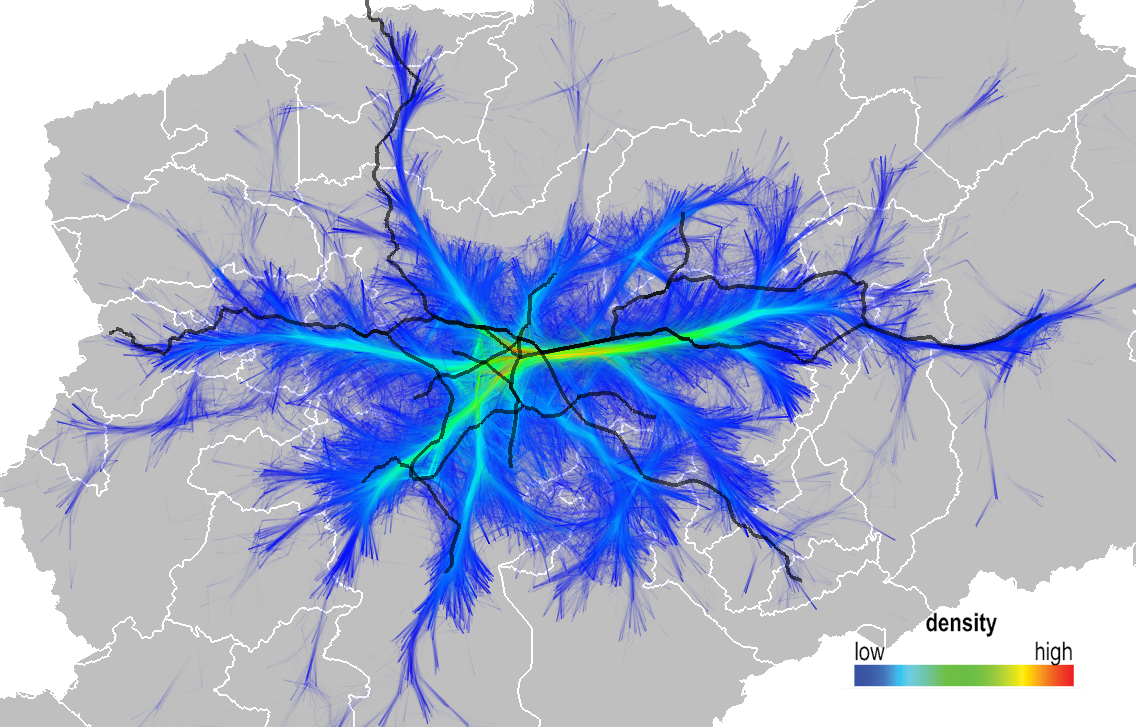
\includegraphics[width=0.98\textwidth]{../figuras/rail-lines.png}
    \caption{\emph{Bundling} das trajetórias coloridas pela densidade e a malha ferroviária da RMSP}
  \label{fig:rails}  
\end{figure}

\section{Mapeando distância e direção no \emph{bundling}}
\label{sec:length-direction}

Para explorar a mobilidade urbana por diferentes perspectivas, precisamos de
meios para visualizar os múltiplos atributos dos dados. Dois
importantes atributos para o estudo de padrões de mobilidade são distância
percorrida na viagem e a sua direção. As Figuras~\ref{fig:attributes-length} e
\ref{fig:attributes-direction} mostram a visualização de todo o conjunto de
dados OD17 mapeando a distância e direção, respectivamente.

Na Figura~\ref{fig:attributes-length} codificamos nas cores os comprimentos das
viagens. Nela utilizamos o mesmo mapa de cores (arco-íris) da
Figura~\ref{fig:rails}, além também de aplicar a modulação da transparência por densidade,
conforme explicado na Seção~\ref{sec:density}. Nesta imagem, podemos observar
uma única curva vermelha aparentemente na horizontal. Sua alta opacidade implica
que há muitas viagens longas, todas mapeadas perfeitamente para essa trajetória
entre a mesma origem e destino (se não o fizessem, veríamos um \emph{bundle} se
ramificando no formato de um leque em vez de uma curva precisa). Esta é uma
descoberta interessante que, argumentamos, não poderia ser facilmente encontrada
usando métodos não visuais. Apesar desse ponto fora do comum, as outras trajetórias,
em geral, percorrem distâncias regulares. \emph{Bundles} de longa distância como
este podem indicar falta de serviços ou recursos que não satisfazem as regiões
locais, obrigando as pessoas a percorrerem longas distâncias para acessá-los. A
pesquisa OD17 contém mais informações que podem ajudar a investigar o motivo
dessas longas viagens.

A Figura~\ref{fig:attributes-direction} mostra os mesmos dados da
Figura~\ref{fig:attributes-length}, mas ao invés da distância são as direções
das viagens que estão codificadas em cores. Para este atributo em específico,
usamos ainda um recurso do \emph{CUBu}, que separa trilhas em direções opostas
em dois \emph{bundles} quase paralelos. Podemos ver claramente a existência de
trajetórias paralelas ao longo dos \emph{bundles}, o que não é surpreendente
porque a pesquisa OD registra o trajeto típico das pessoas que inclui os
deslocamentos de ida e vinda de volta para suas origens. No entanto, essa
simetria das trajetórias não é observada quando analisamos períodos
específicos do dia, como mostramos na Seção~\ref{sec:peak-hours}.

\begin{figure}[!htb] \centering \captionsetup{justification=centering}
  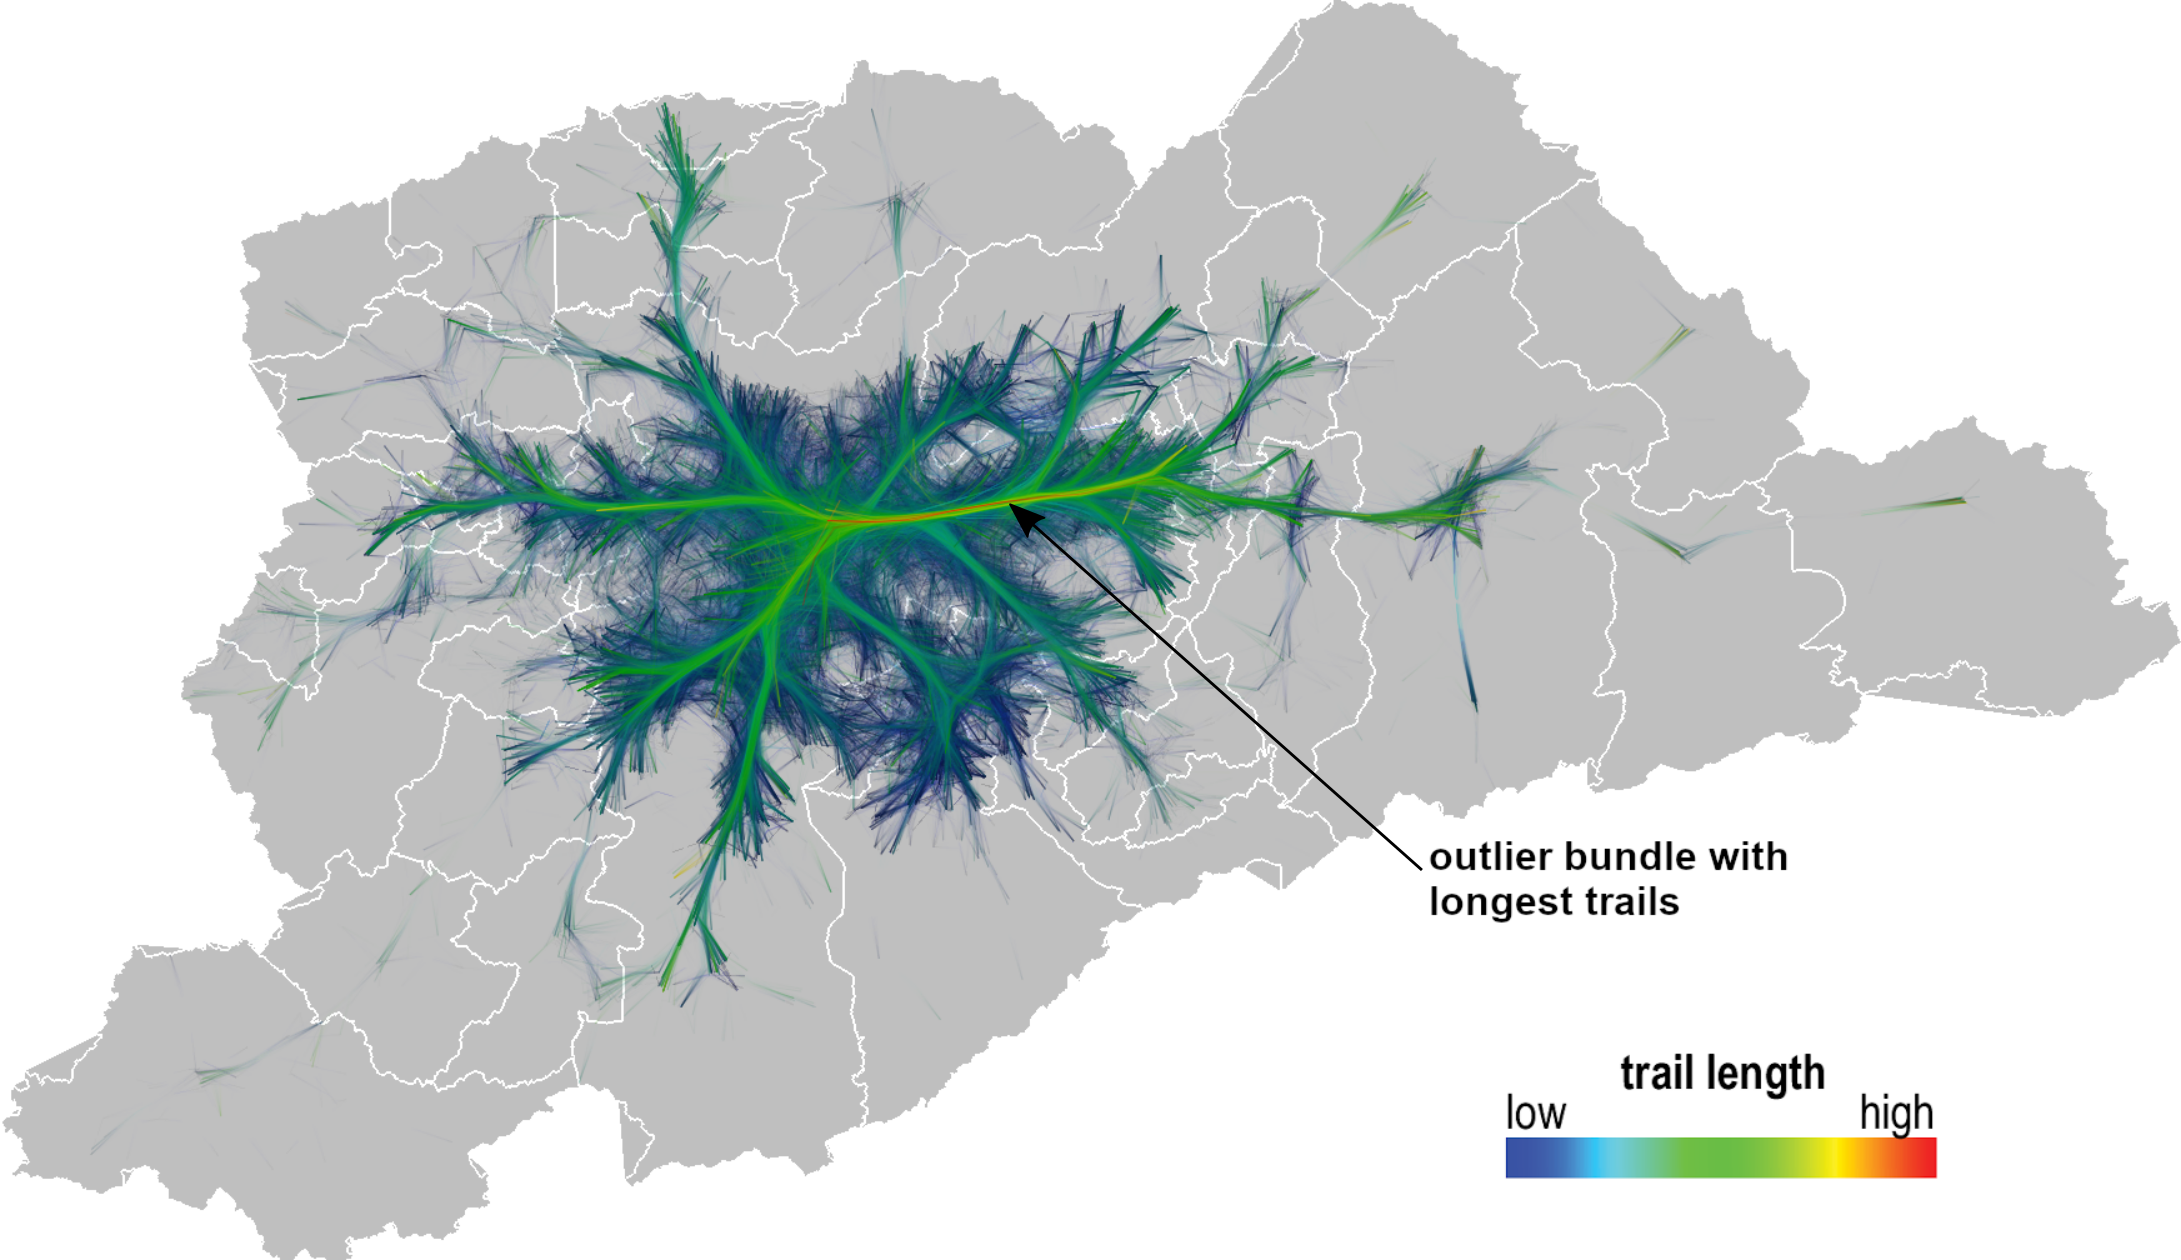
\includegraphics[width=0.98\textwidth]{../figuras/distances.png}
  \caption{Mapeamento da distância das viagens em cores. \label{fig:attributes-length}}
  \end{figure}

\begin{figure}[!htb]
  \centering
  \captionsetup{justification=centering}
  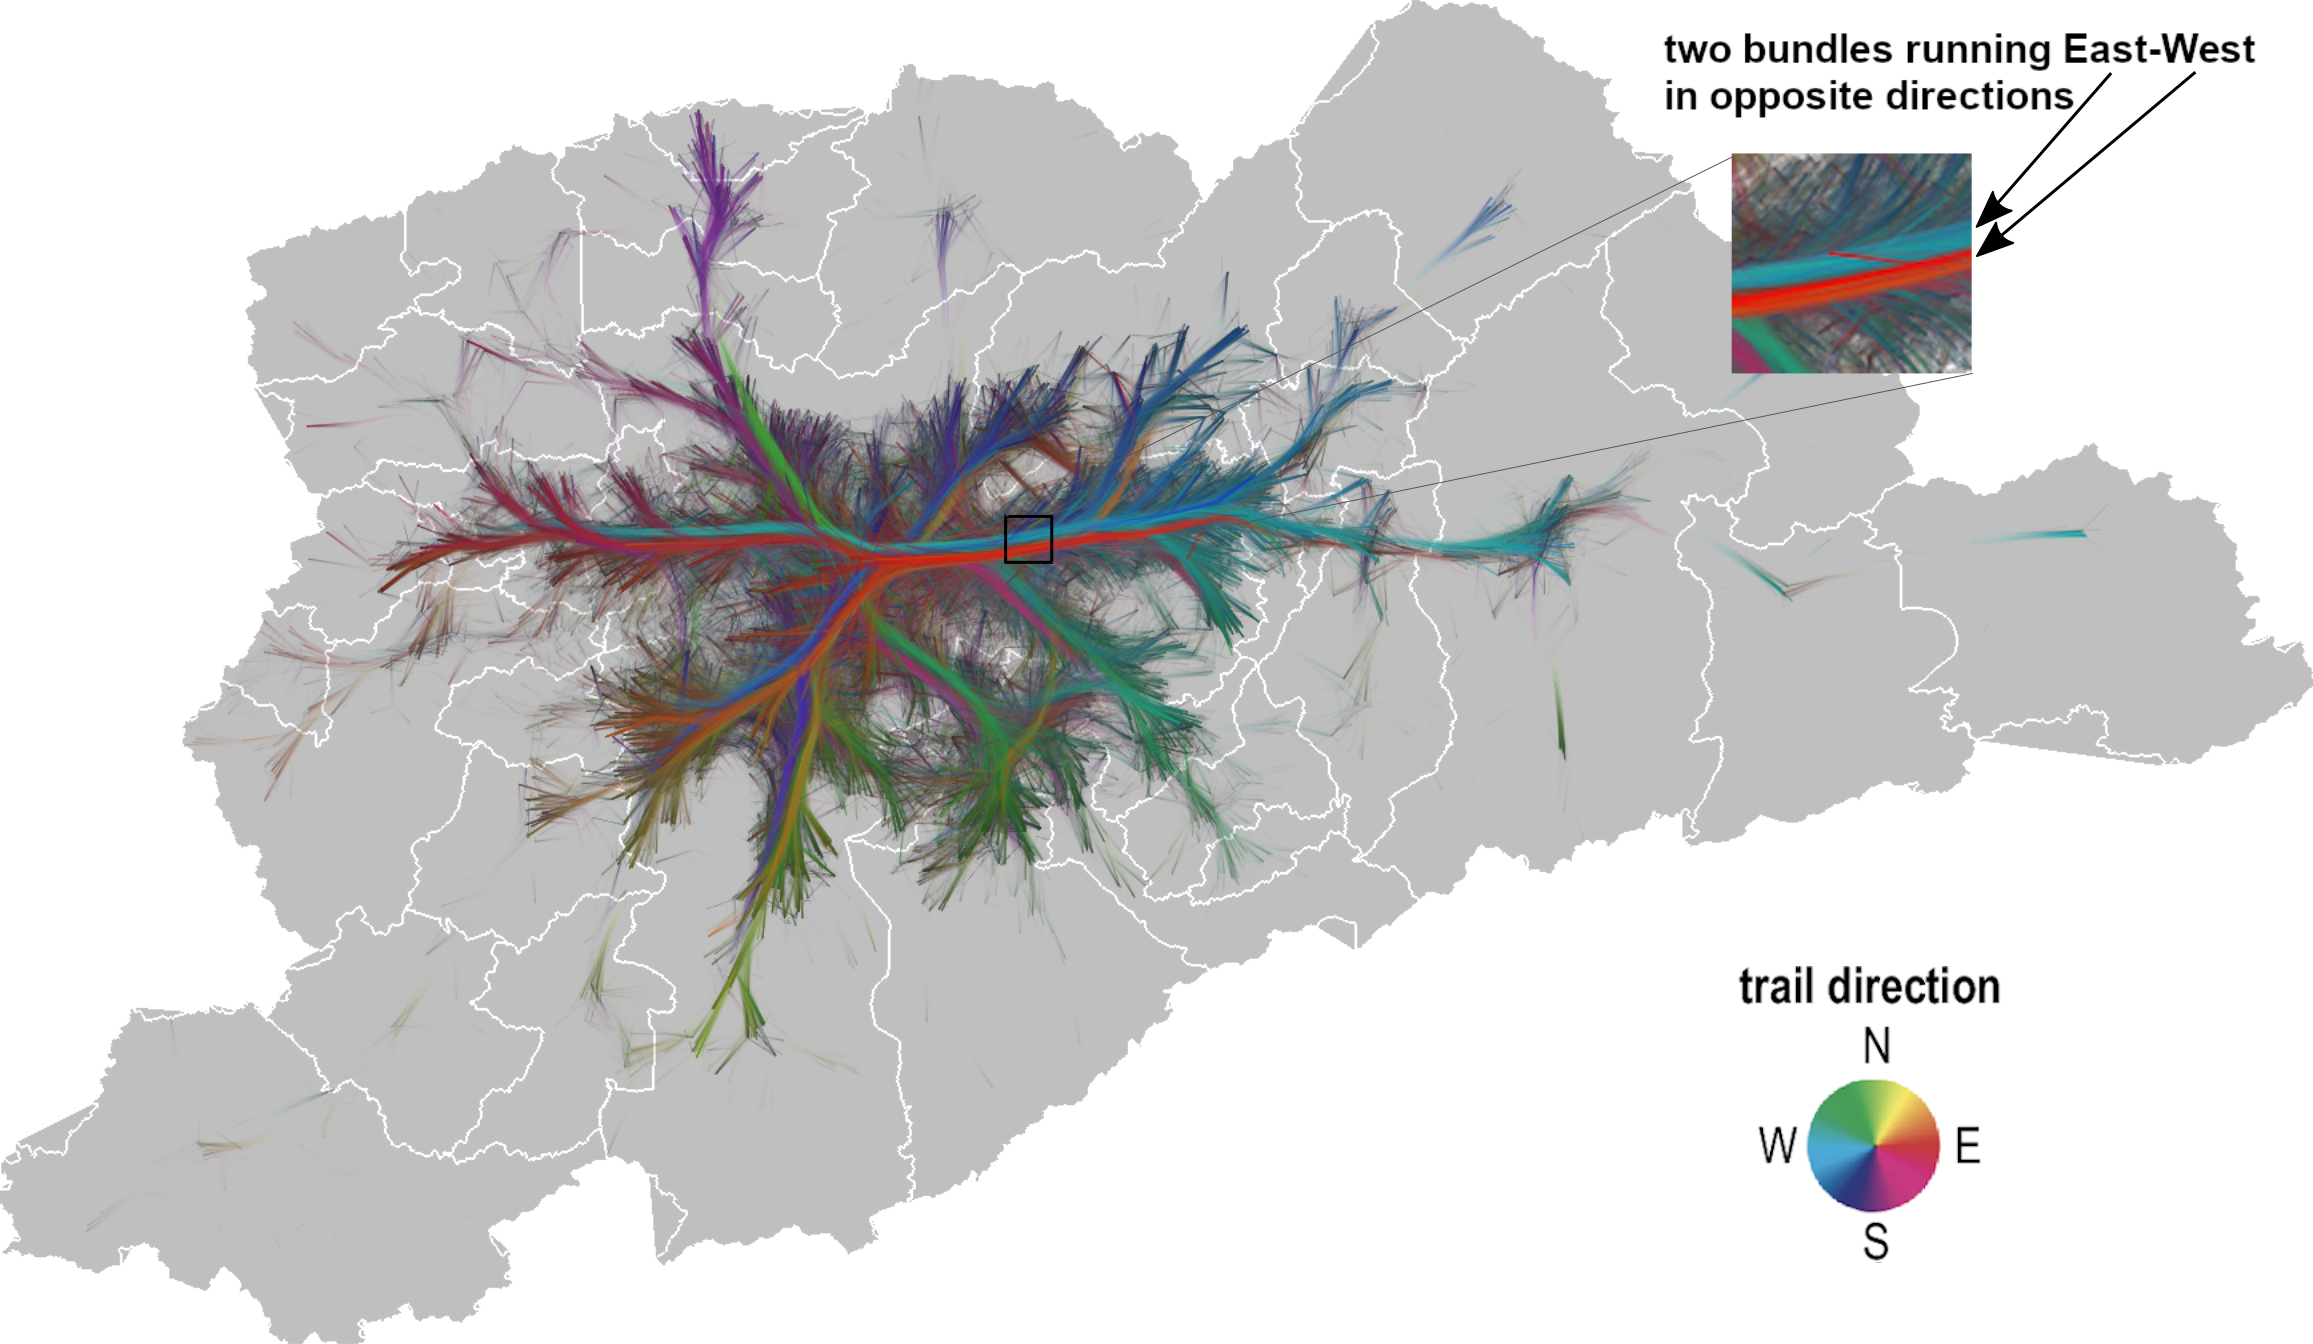
\includegraphics[width=0.98\textwidth]{../figuras/directions.png}
  \caption{Mapeamento da direção das viagens em cores. \label{fig:attributes-direction}}
\end{figure}

\section{Visualização dos modos de transporte: ônibus locais \emph{vs.} intermunicipais}
\label{sec:coloring}

Como mostramos na Seção~\ref{sec:pesquisa-od}, o conjunto de dados OD17 contém
17 modos de transporte. Embora fosse ideal ser capaz de ver as 17 categorias ao
mesmo tempo em nossa visualização com \emph{bundling}, isso não seria fácil de
se obter, uma vez que exigiria a codificação simultânea de 17 diferentes
categorias de transporte. Então, nós utilizamos a transparência para esconder
trajetórias de acordo com seletores que podem ser configurados na interface para
filtrar as trajetórias pelo modo de transporte, como mostra a Figura~\ref{fig:filtros-modes}
a seguir.

\begin{figure}[!h]
  \centering
  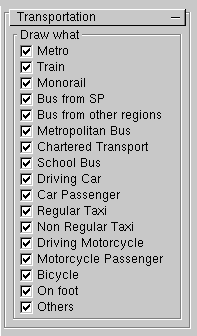
\includegraphics[width=.27\textwidth]{../figuras/filtros-modes.png}
  \caption{Filtros de transparência na interface do \emph{CUBu} para seleção dos modos de transporte.}
   \label{fig:filtros-modes}
 \end{figure}

Assim, na Figura~\ref{fig:bus-integration} mostramos como utilizamos tais
filtros que utilizamos para visualizar a integração entre os ônibus da cidade de
São Paulo (ônibus locais) e os ônibus intermunicipais. As trajetórias originais
e agrupadas com \emph{bundling} são apresentadas lado a lado. Cada meio de
transporte tem uma coloração distinta - verde para ônibus locais e azul para
ônibus intermunicipais. Podemos ver mais claramente na
Figura~\ref{fig:bus-integration-zoom} (zoom) que esses diferentes sistemas de
transporte parecem se complementar. A cidade de São Paulo tem um comércio e uma
indústria muito ativa, que recebe muitos trabalhadores advindos das cidades
vizinhas. Assim, a disponibilidade de transporte público e sua integração é
muito importante para essas pessoas. Esse tipo de filtragem juntamente com as
técnicas de \emph{bundling} ajudam a entender melhor as correlações entre os
atributos dos dados - neste caso, modos de transporte.


\begin{figure}[!htb]
  %\centering
  %\raggedright\noindent\hspace{-\margemesq}\hspace{.01\paperwidth}%
  %\begin{subfigure}{0.49\paperwidth}
  \raggedright\noindent\hspace{-.02\textwidth}%
  \begin{subfigure}{0.55\textwidth}
    \centering
    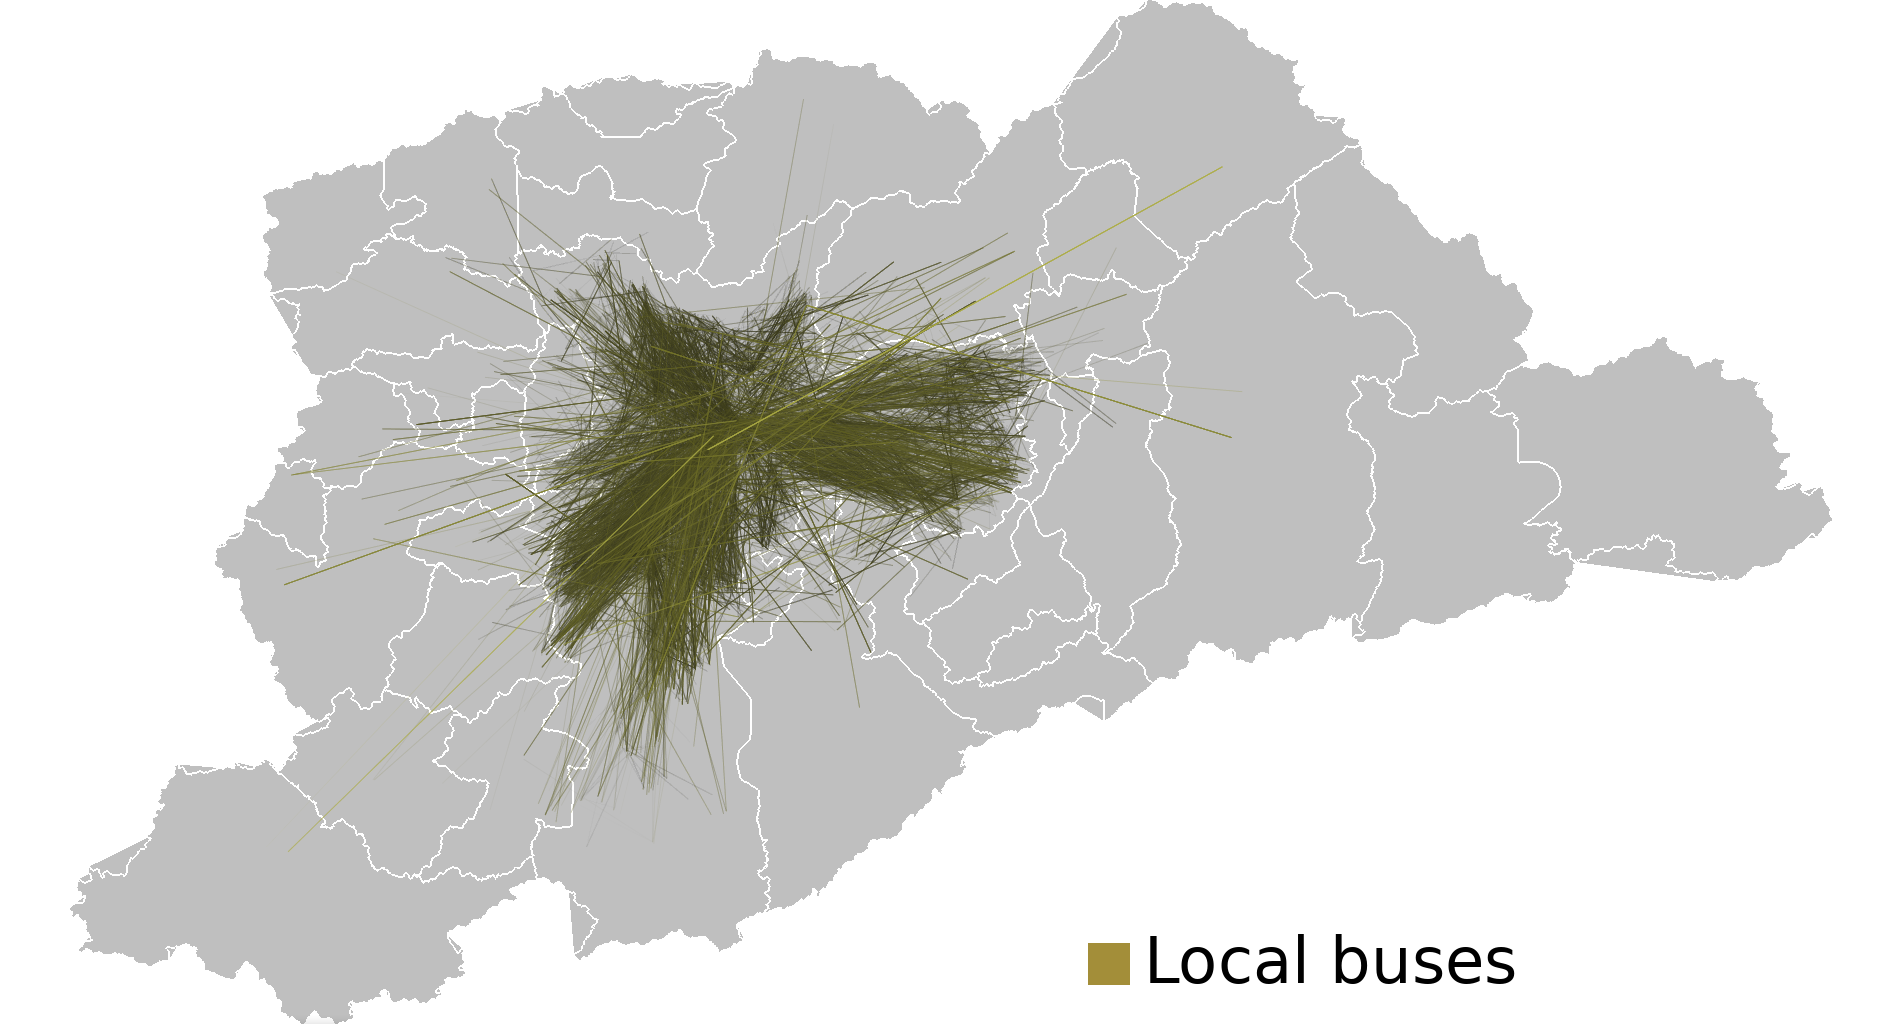
\includegraphics[width=1\textwidth]{../figuras/busesLocalXmetropolitan/unbundled-buses.png}
    \caption{\label{fig:bus-integration-a}}
  \end{subfigure}\nobreak%
  %\begin{subfigure}{0.49\paperwidth}
  \hspace{-.06\textwidth}\nobreak%
  \begin{subfigure}{0.55\textwidth}
    \centering
    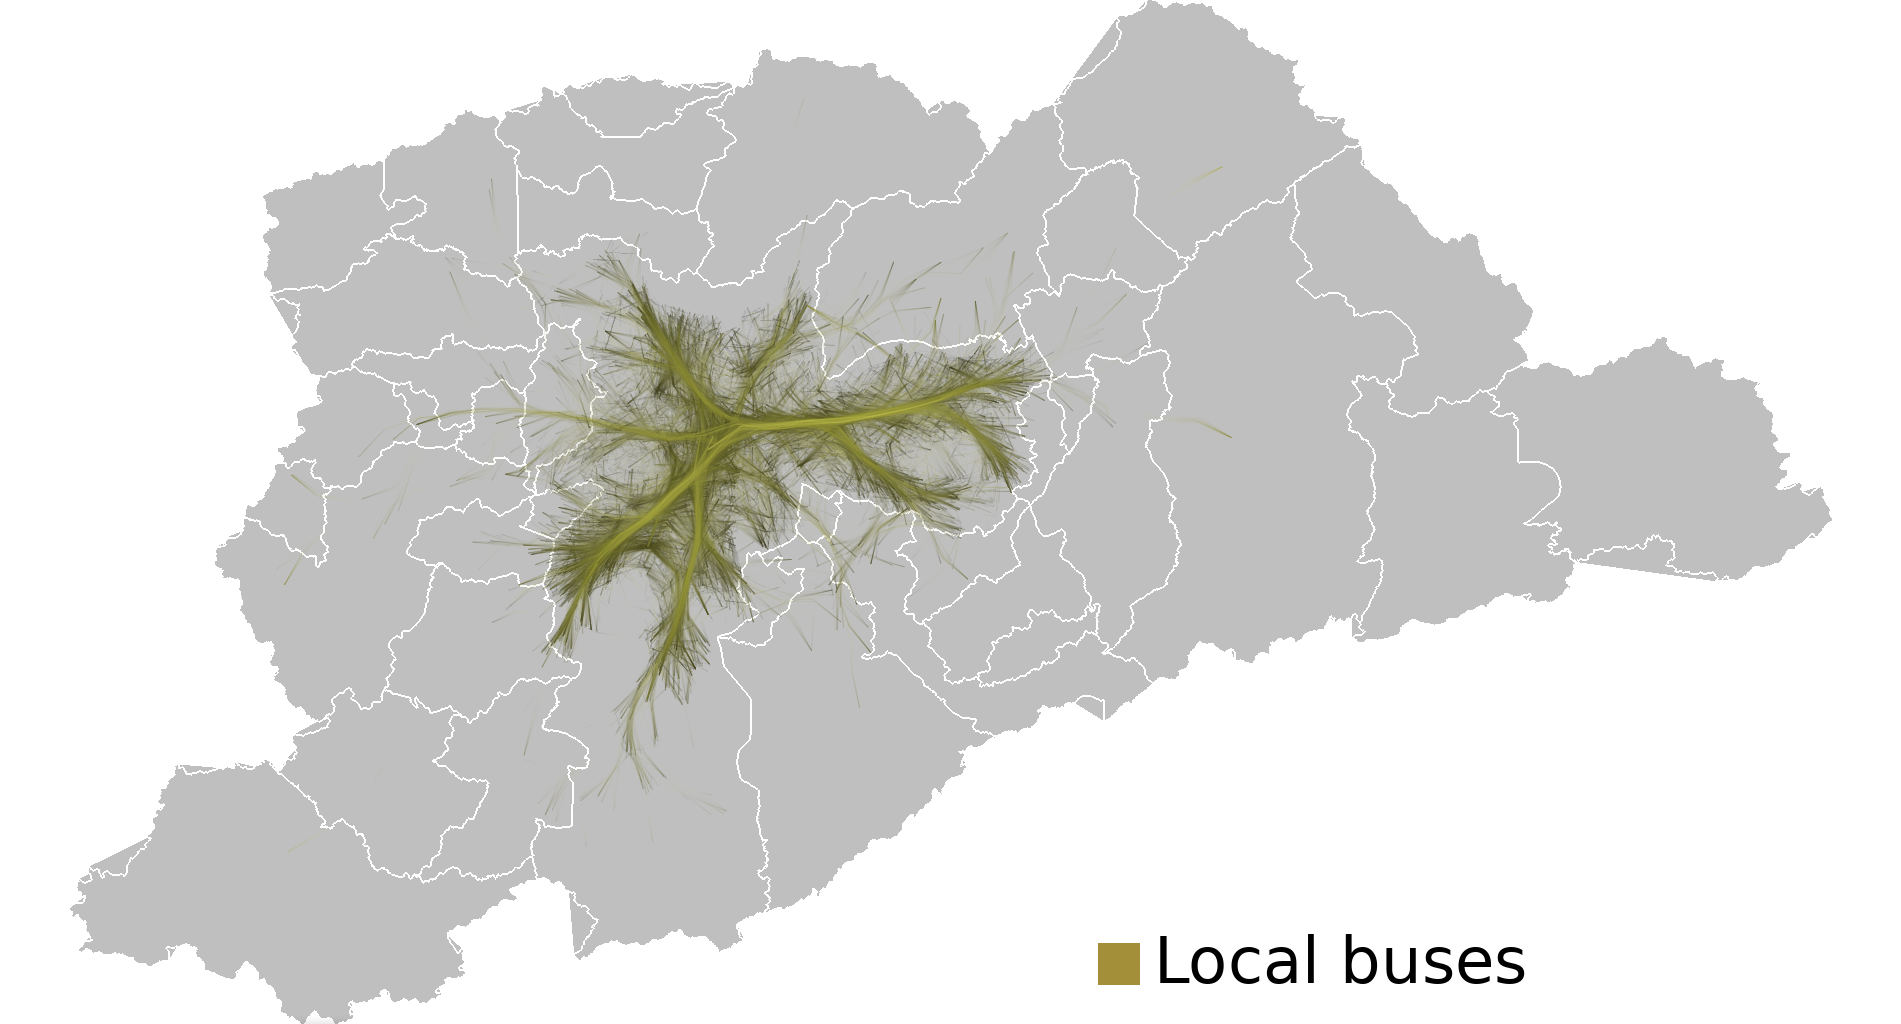
\includegraphics[width=1\textwidth]{../figuras/busesLocalXmetropolitan/bundled-buses-length.png}
    \caption{\label{fig:bus-integration-b}}
  \end{subfigure}

  %\noindent\hspace{-\margemesq}\hspace{.01\paperwidth}\begin{subfigure}{0.49\paperwidth}
  \raggedright\noindent\hspace{-.02\textwidth}%
  \begin{subfigure}{0.55\textwidth}
    \centering
    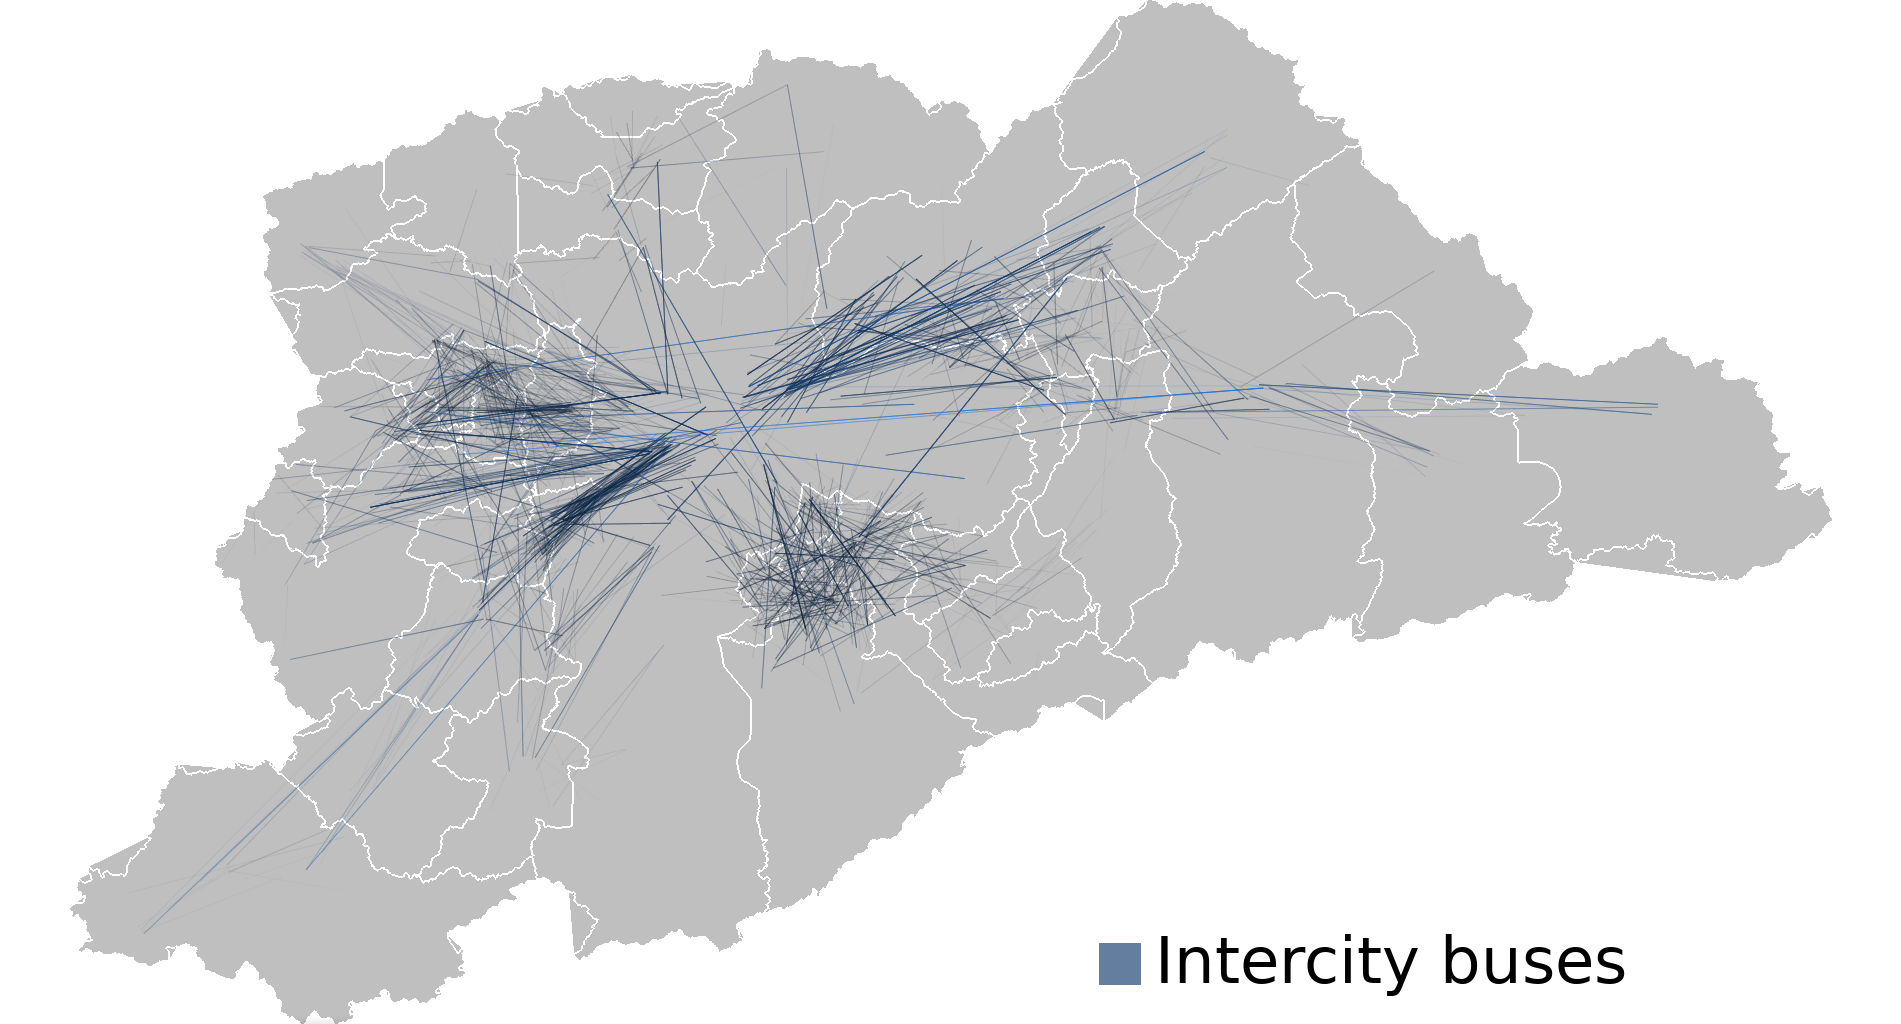
\includegraphics[width=1\textwidth]{../figuras/busesLocalXmetropolitan/unbundled-metropolitan-buses.png}
    \caption{\label{fig:bus-integration-c}}
  \end{subfigure}\nobreak%
  \hspace{-.06\textwidth}\nobreak%
  \begin{subfigure}{0.55\textwidth}
  %\begin{subfigure}{0.49\paperwidth}
    \centering
    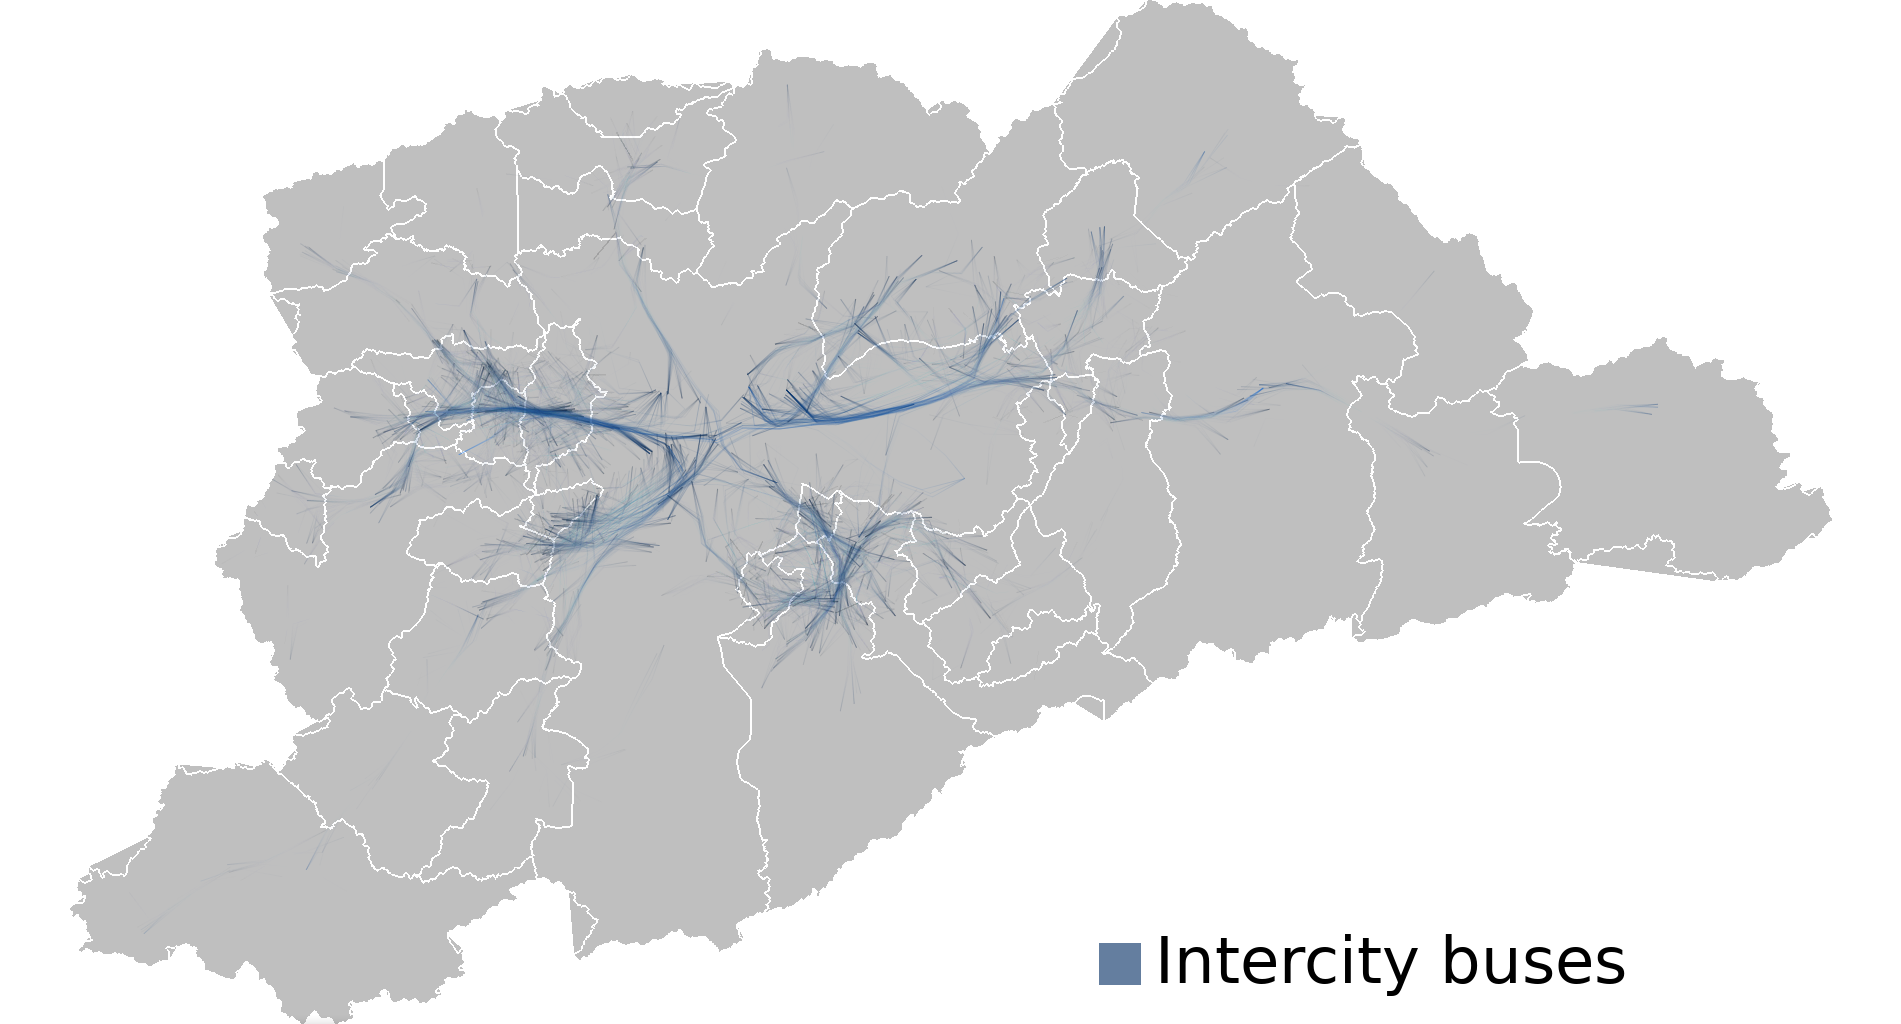
\includegraphics[width=1\textwidth]{../figuras/busesLocalXmetropolitan/bundled-metropolitan-buses-length.png}
    \caption{ \label{fig:bus-integration-d}}
  \end{subfigure}

  %\noindent\hspace{-\margemesq}\hspace{.01\paperwidth}\begin{subfigure}{0.49\paperwidth}
  \raggedright\noindent\hspace{-.02\textwidth}%
  \begin{subfigure}{0.55\textwidth}
    \centering
    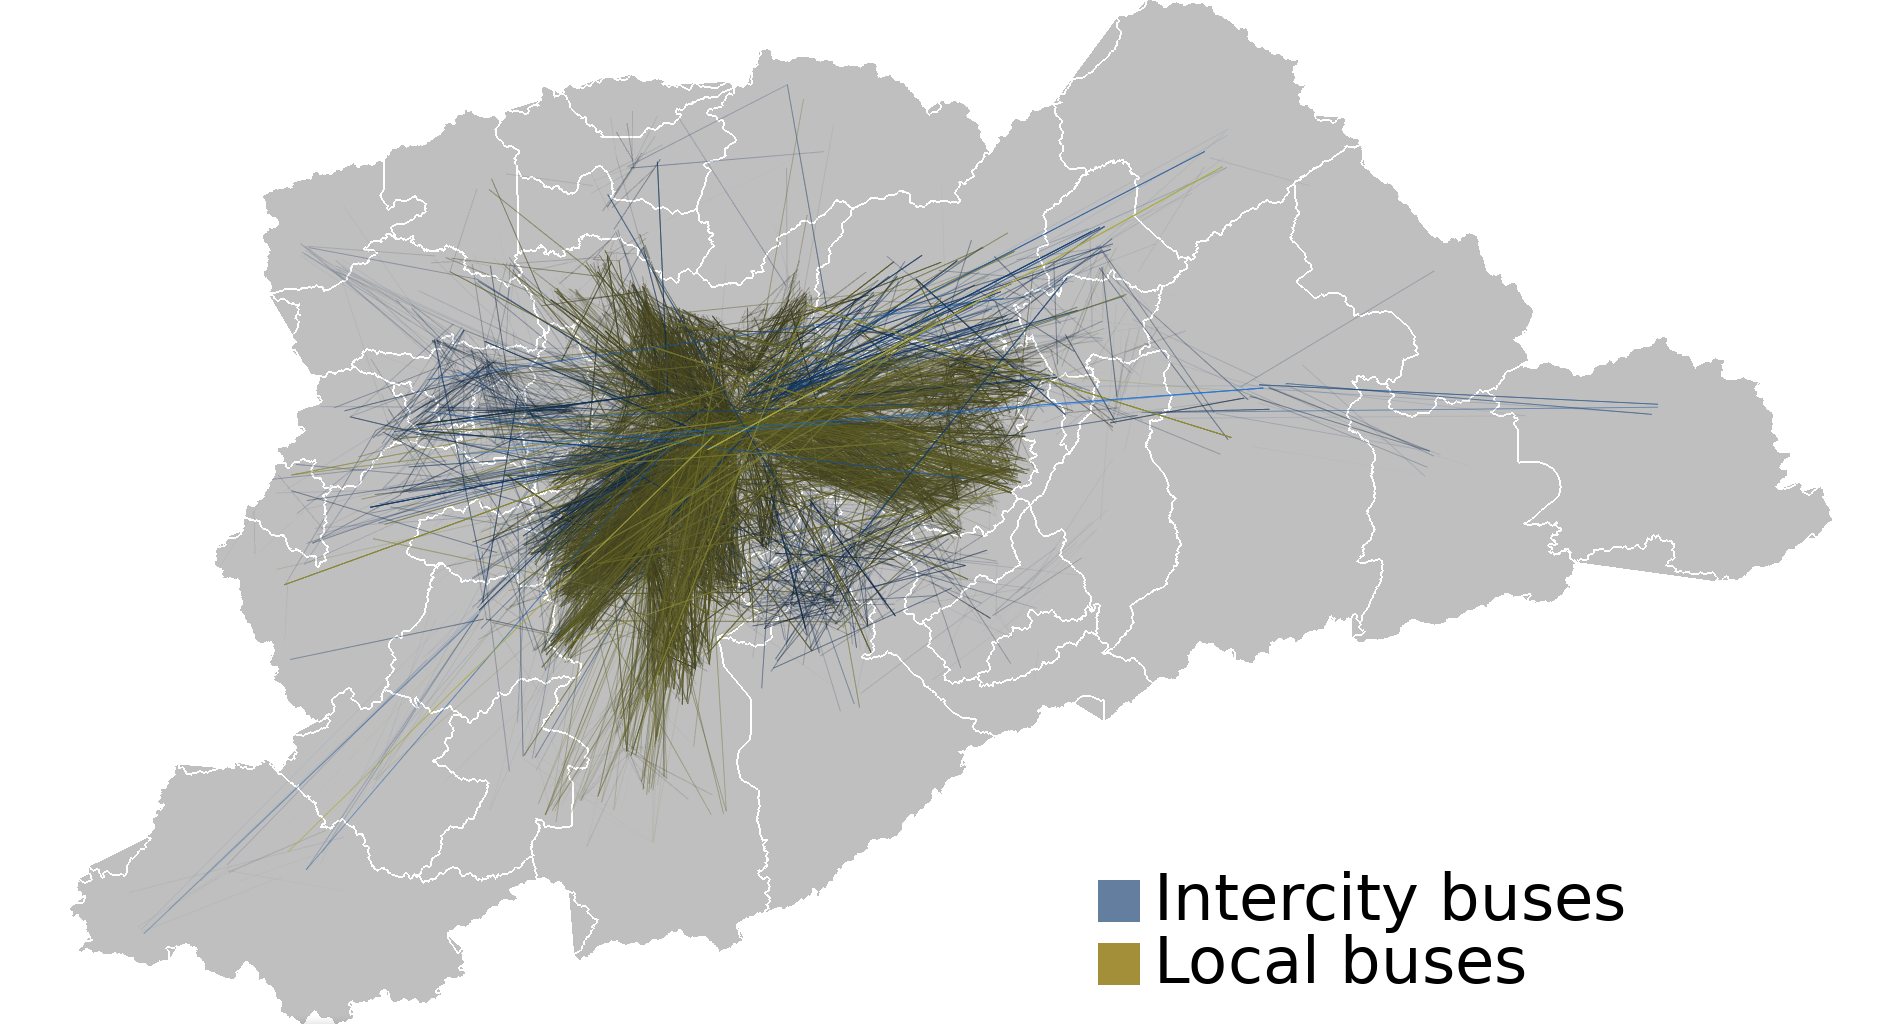
\includegraphics[width=1\textwidth]{../figuras/busesLocalXmetropolitan/unbundled-buses-and-metropolitan.png}
    \caption{\label{fig:bus-integration-e}}
  \end{subfigure}\nobreak%
  \hspace{-.06\textwidth}\nobreak%
  \begin{subfigure}{0.55\textwidth}
  %\begin{subfigure}{0.49\paperwidth}
    \centering
    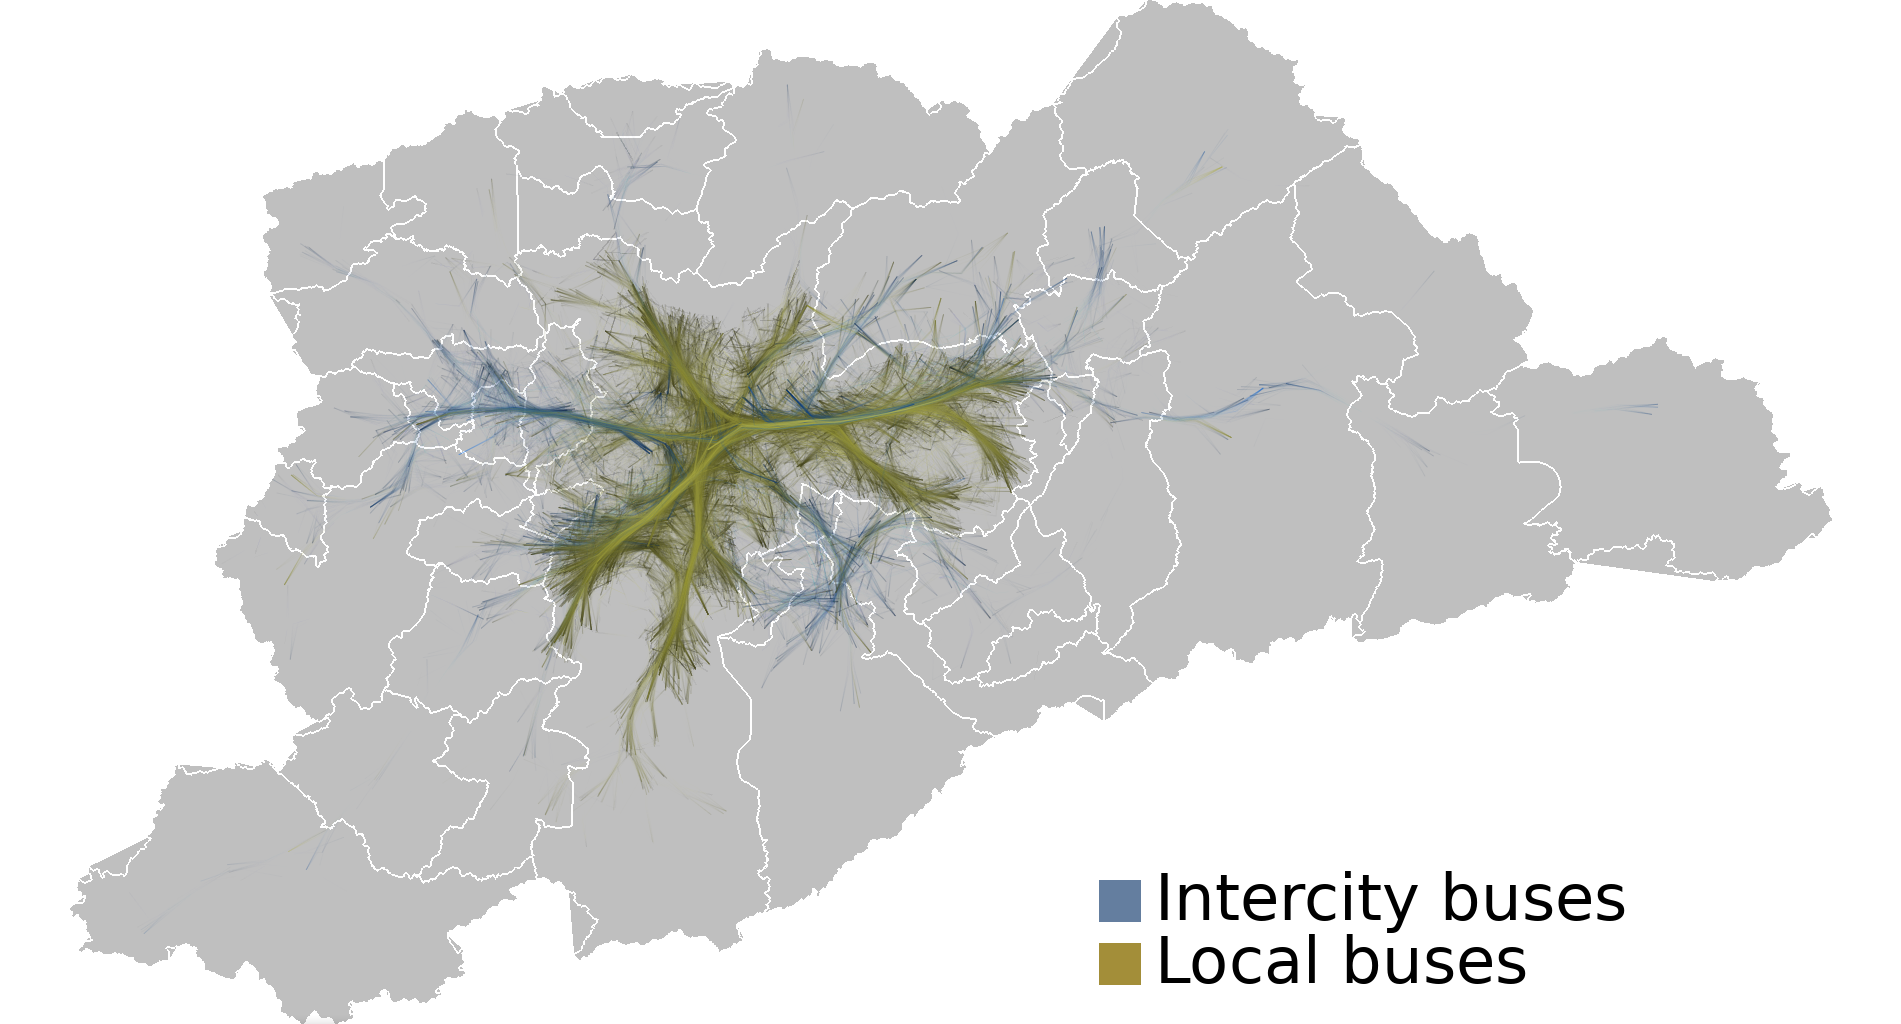
\includegraphics[width=1\textwidth]{../figuras/busesLocalXmetropolitan/bundled-buses-and-metropolitan-length.png}
    \caption{\label{fig:bus-integration-f}}
  \end{subfigure}
  \caption{Viagens filtradas pelo modo de transporte: ônibus locais e intermunicipais. Dados originais à esquerda (a, c, e)  e \emph{bundling} à direita (b, d, f). \label{fig:bus-integration}}
\end{figure}

\begin{figure}[!htb]
  \centering
  \captionsetup{justification=centering}
  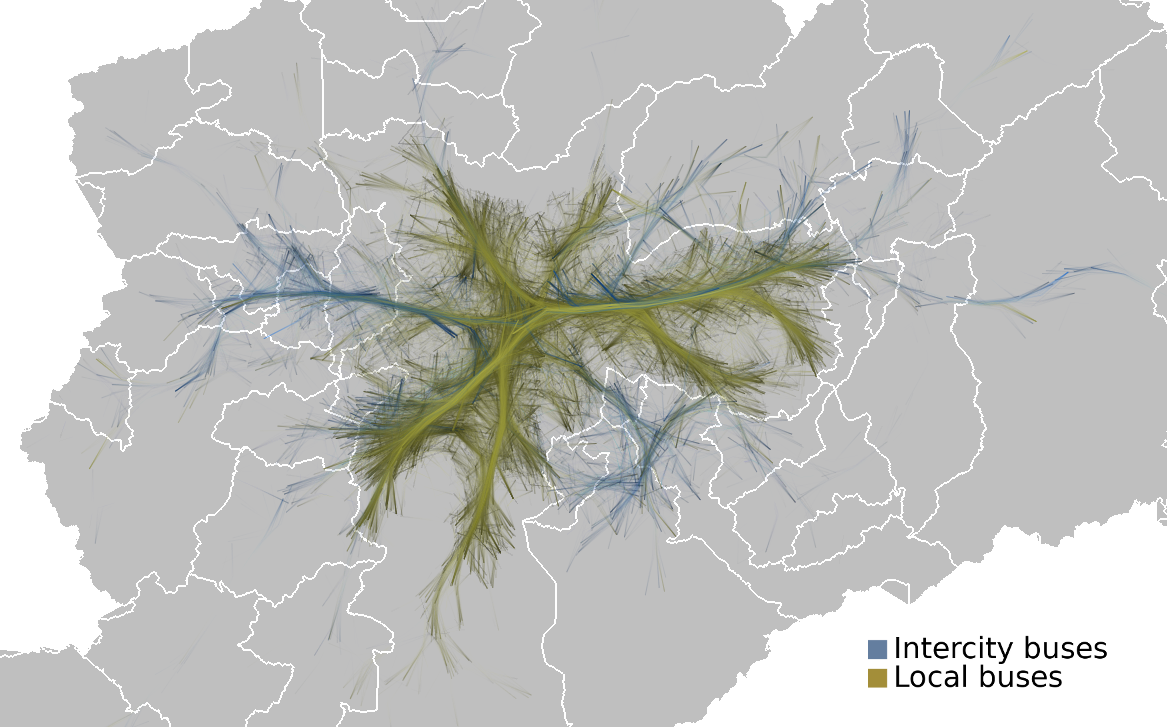
\includegraphics[width=0.98\textwidth]{../figuras/local-intercity-buses}
  \caption{Viagens filtradas pelo modo de transporte: ônibus locais e intermunicipais (zoom). \label{fig:bus-integration-zoom}}
\end{figure}

\section{Visualização das diferentes classes sociais}
\label{sec:strata}

Usamos nossa visualização com \emph{bundling} para estudar como os cidadãos com diferentes
condições econômicas se deslocam na RMSP. O Critério de Classificação Econômica
Brasileira (CCEB), \citep{cceb2008} é o índice socioeconômico oficial utilizado no Censo
Demográfico Brasileiro, realizado pelo Instituto Brasileiro de Geografia e
Estatística (IBGE). Ele mede o poder de compra da sociedade brasileira. O CCEB é
dividido em seis níveis (ou classes) (Tabela~\ref{tab:becc}). Este índice é usado na pesquisa
OD17 para complementar os dados de mobilidade. A Tabela~\ref{tab:becc} também mostra a renda
média mensal (em reais), e o número de viagens na RMSP para cada nível do CCEB considerando toda a população e apenas
os cidadãos com idade entre 6 e 18 anos que se deslocam para fins de estudos (consulte a
Seção~\ref{sec:students}). O motivo pelo qual o total de viagens na tabela ser abaixo de 42 milhões
é que muitos registros do conjunto de dados não tinham a informação da sua classificação no CCEB, e por isso
não foram considerados no cálculo.

\begin{table}[!htb]
  \small
  \newcommand{\hdr}[1]{\bfseries#1}
  \centering
  \caption{Quantidade de viagens pelo índice CCEB (2017), renda mensal e idade. \label{tab:becc}}
  \begin{tabular}{>{\footnotesize}c>{\footnotesize}r>{\footnotesize}r>{\footnotesize}r>{\footnotesize}r}
    \toprule
    \multirow{2}[2]{*}{\hdr{Nível CCEB}} & \hdr{Renda mensal} & \hdr{Viagens} & \hdr{Viagens de estudantes}\\
    & \hdr{em reais (R\$)} & \hdr{totais} & \hdr{entre 6 e 18 anos}\\
    \midrule
    A   & 23,345    & 3,062,892  &   184,772\\
    B1  & 10,386    & 3,854,040  &   260,652\\
    B2  & 5,363     & 12,856,182 &   963,242\\
    C1  & 2,965     & 11,277,159 &   976,745\\
    C2  & 1,691     & 7,852,806  &   721,218\\
    D-E & 708       & 2,233,801  &   219,612\\
    \textbf{Total}& n/a & 411,368,80 &  3,326,241\\
    \bottomrule
  \end{tabular}
\end{table}

Para comparar os padrões de mobilidade de diferentes classes sociais CCEB,
aplicamos \emph{bundling} nas viagens de cada classe separadamente, como
mostrado nas Figuras~\ref{fig:becc-axd-e}~até~\ref{fig:becc-d-e}. Observamos
diferenças significativas nos padrões de mobilidade entre os níveis de renda
mais altos e mais baixos, como mostra a Figura~\ref{fig:becc-axd-e}. O nível $A$
(Figura~\ref{fig:becc-a}) apresenta alta densidade no centro da RMSP, que inclui
o entorno do centro da capital. A maior densidade está localizada nos bairros
oeste, sudoeste e nordeste próximos ao centro. Existem fluxos de densidade entre
a capital e as cidades de Barueri e Cotia, que possuem áreas residenciais de
alta renda. Existem outros fluxos de alta densidade ligando a capital às cidades
de São Bernardo do Campo e Santo André. Comparando A ao nível D-E (Figura 18),
vemos que D-E tem os fluxos densos mais elevados na região leste da capital. No
mapa de níveis D-E, podemos ver a ausência de fluxos de alta densidade nas
regiões mais próximas do centro da capital; em contraste, eles estão presentes
no mapa de nível A.

\begin{figure}[!htb]
  \centering
  \captionsetup{justification=centering}
  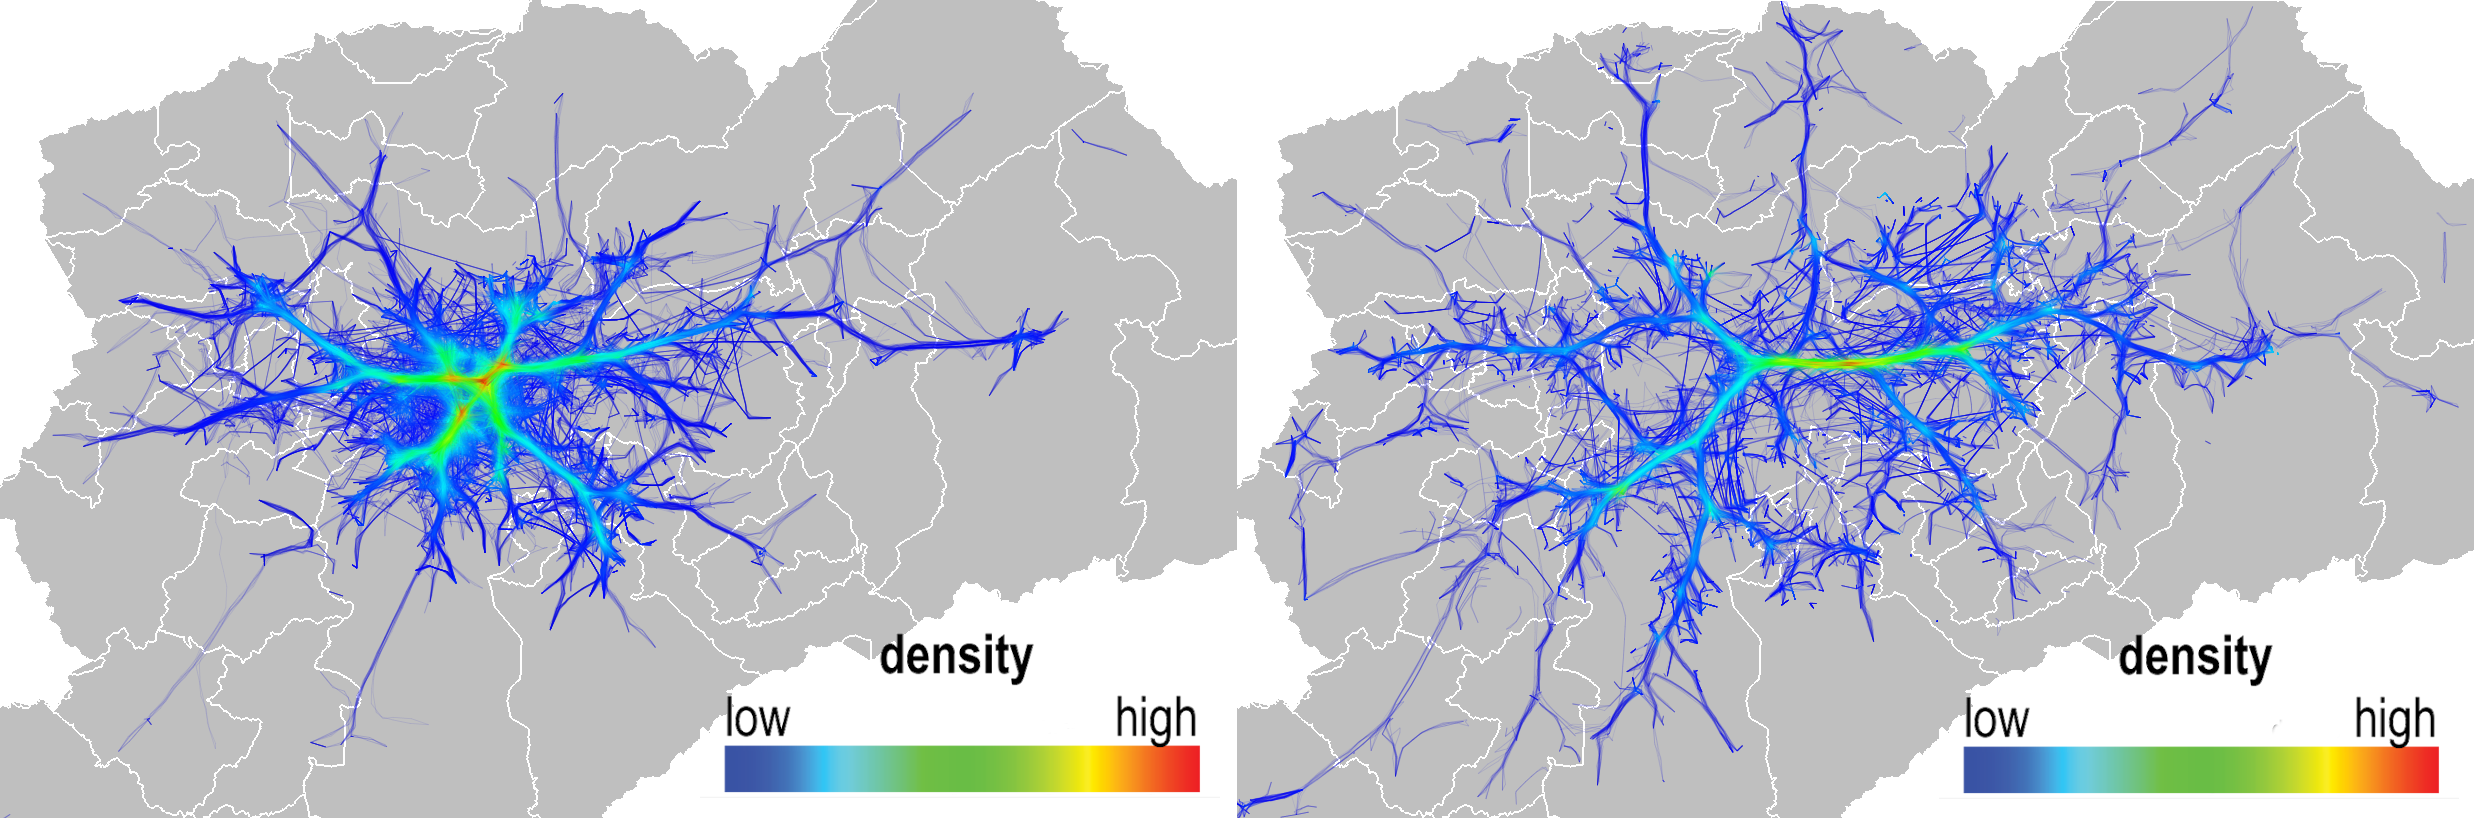
\includegraphics[width=0.98\textwidth]{../figuras/comparison-axd-e-strata-leg.png}
  \caption{Densidade das viagens da classe $A$ (esquerda) e $D$-$E$ (direta). \label{fig:becc-axd-e}}
\end{figure}

\begin{figure}[!htb]
  \centering
  \captionsetup{justification=centering}
  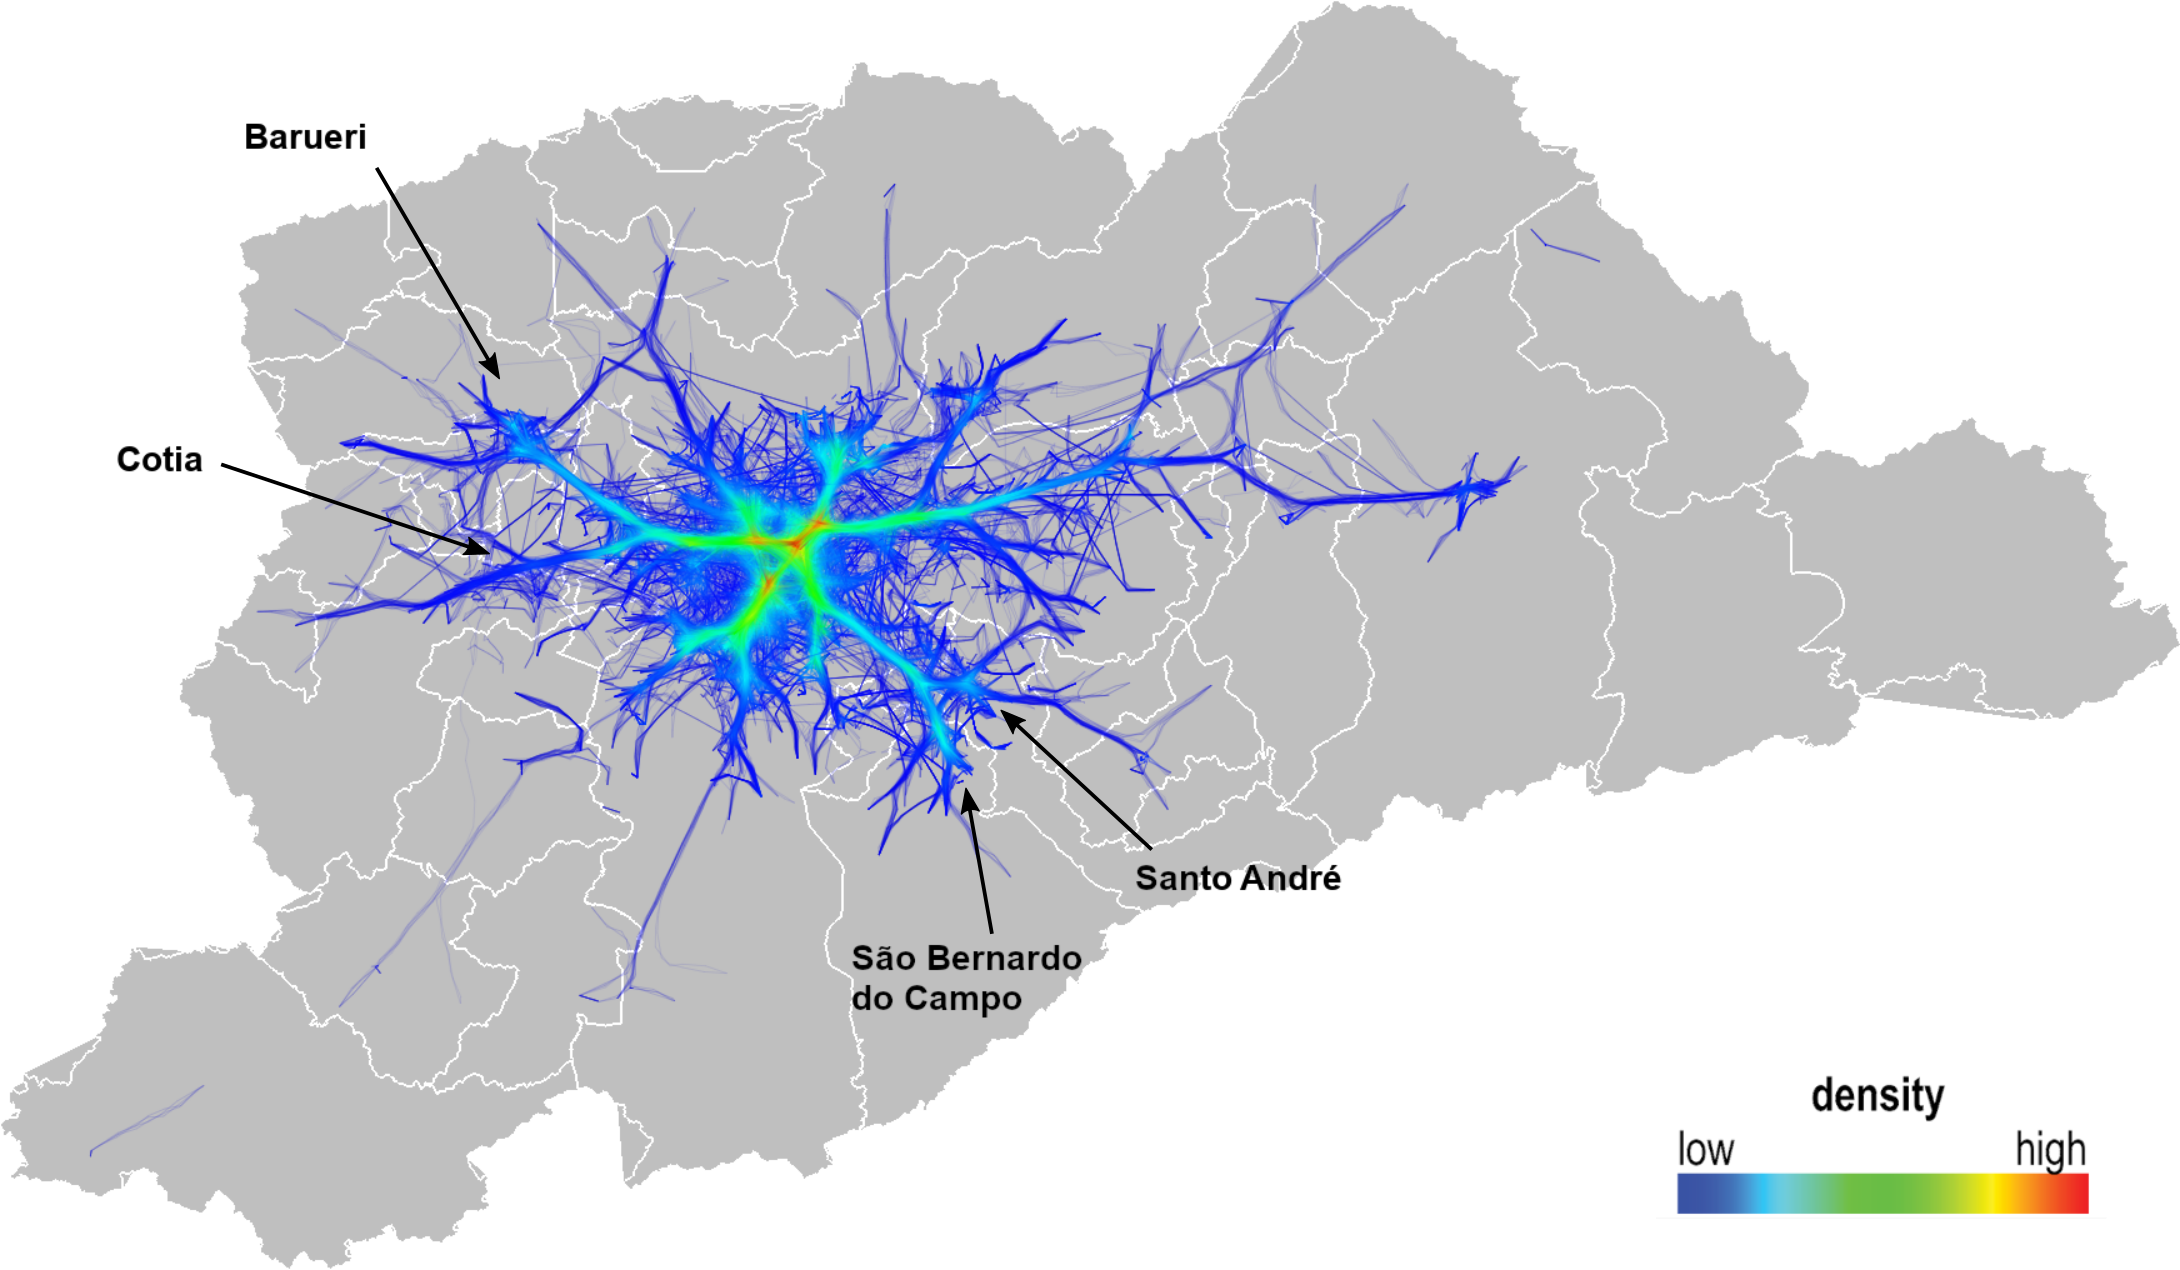
\includegraphics[width=0.98\textwidth]{../figuras/1-class-a.png}
  \caption{Densidade das viagens da classe $A$. \label{fig:becc-a}}
\end{figure}

\begin{figure}[!htb]
  \centering
  \captionsetup{justification=centering}
  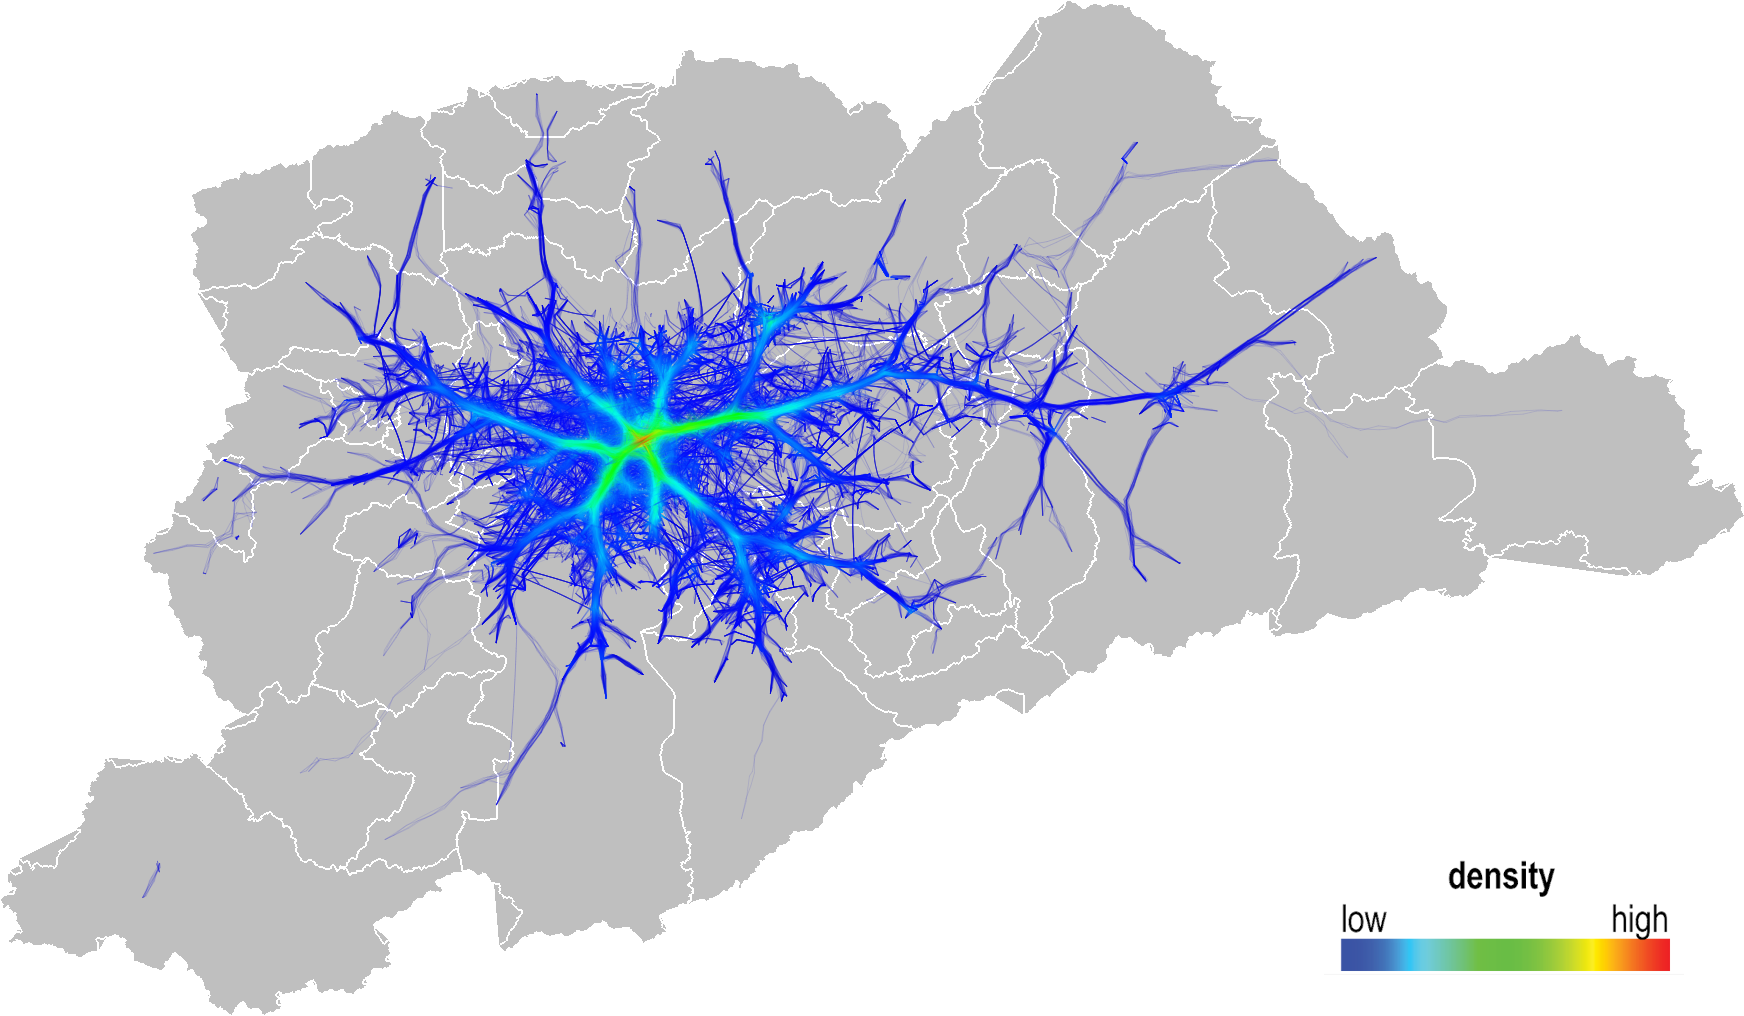
\includegraphics[width=0.98\textwidth]{../figuras/2-class-b1.png}
  \caption{Densidade das viagens da classe $B1$. \label{fig:becc-b1}}
\end{figure}

\begin{figure}[!htb]
  \centering
  \captionsetup{justification=centering}
  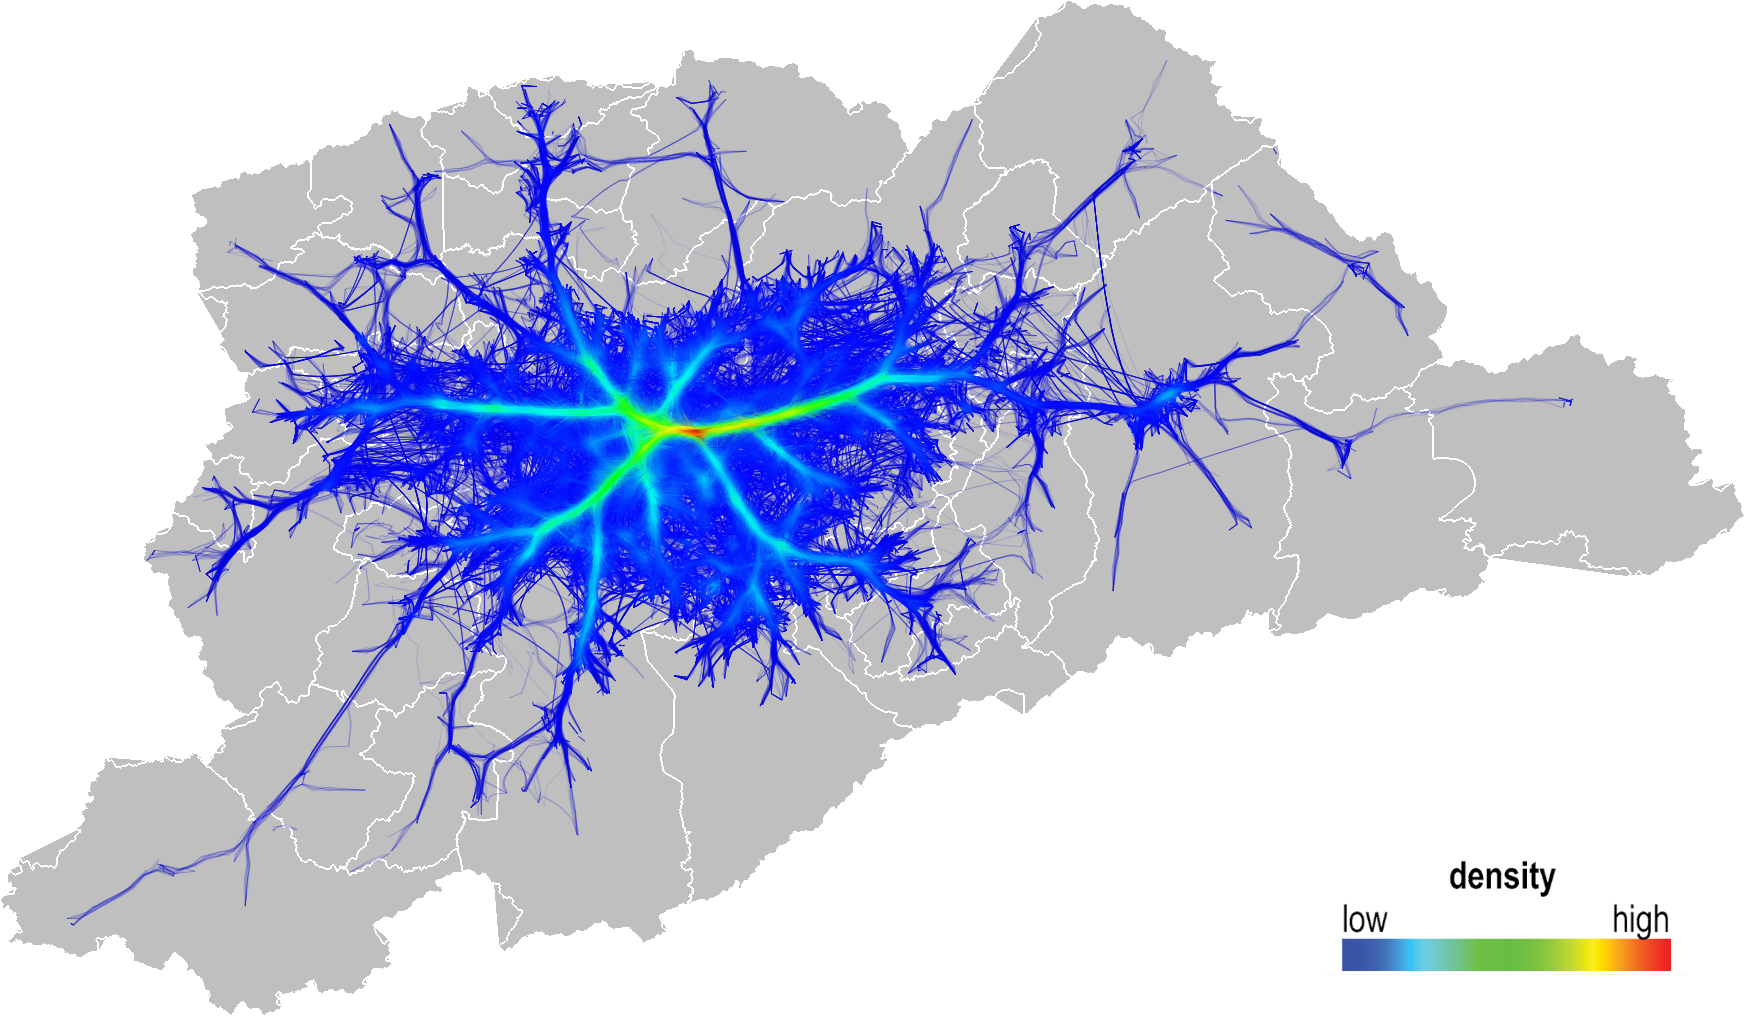
\includegraphics[width=0.98\textwidth]{../figuras/3-class-b2.png}
  \caption{Densidade das viagens da classe $B2$. \label{fig:becc-b2}}
\end{figure}

\begin{figure}[!htb]
  \centering
  \captionsetup{justification=centering}
  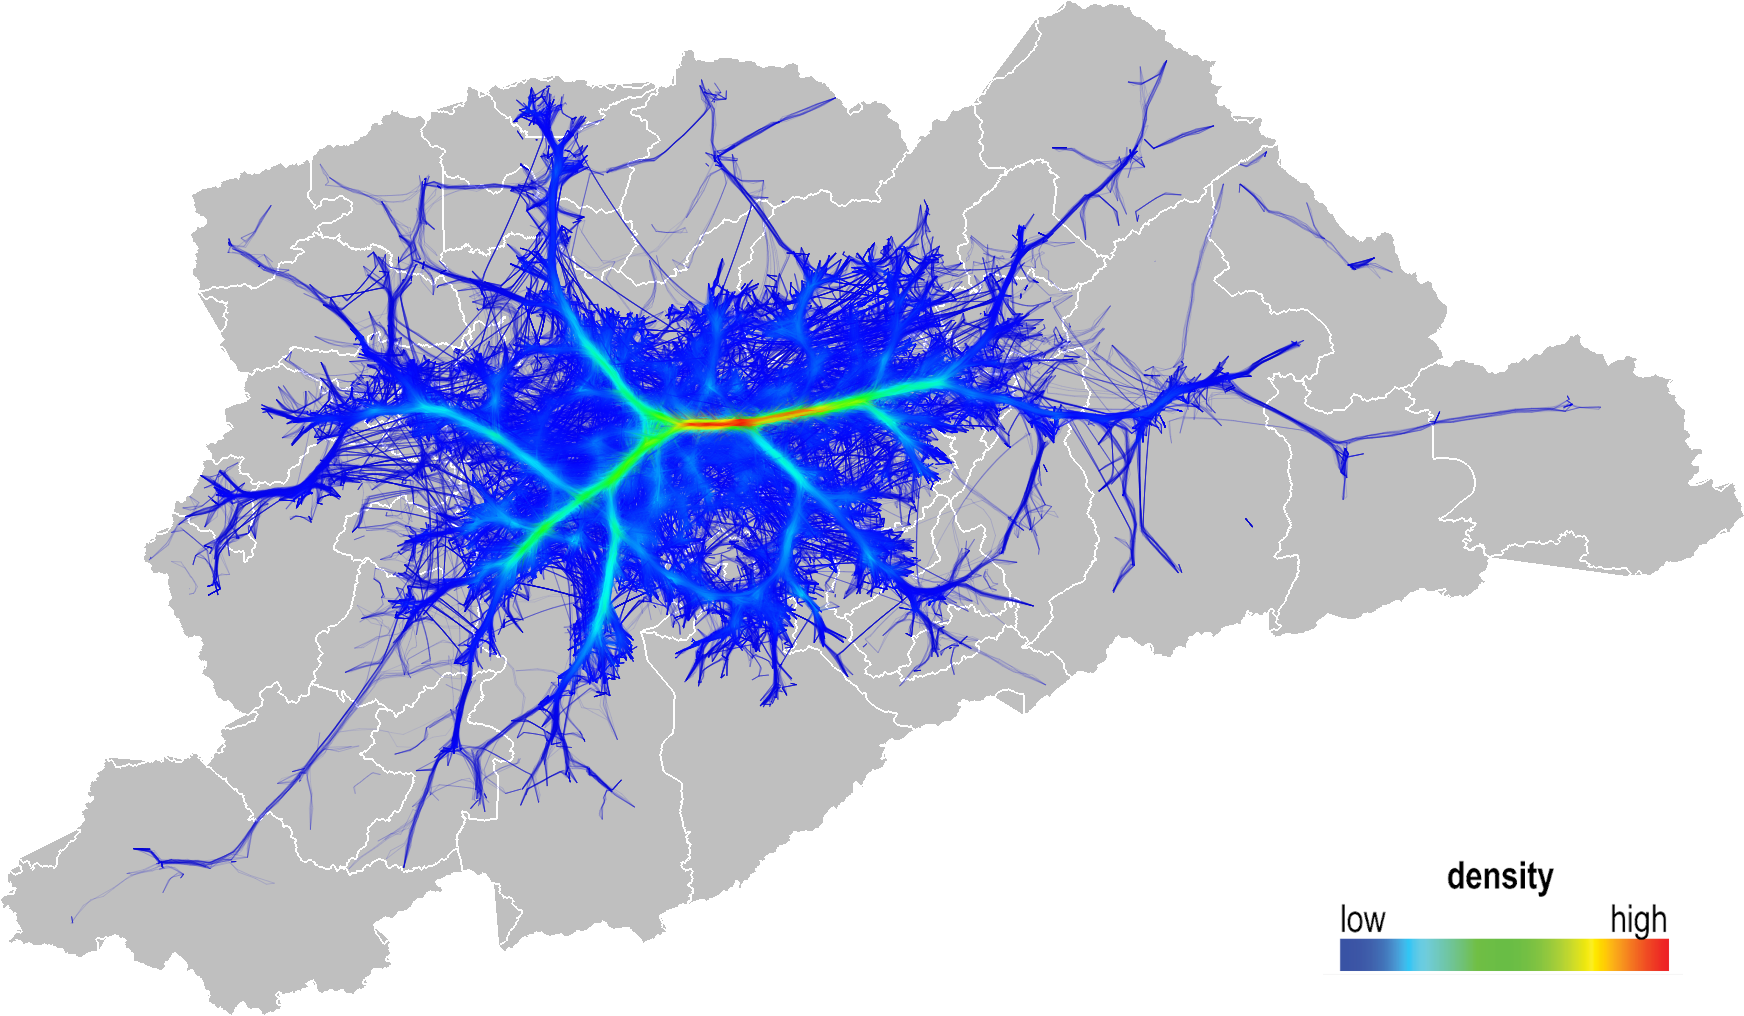
\includegraphics[width=0.98\textwidth]{../figuras/4-class-c1.png}
  \caption{Densidade das viagens da classe $C1$. \label{fig:becc-c1}}
\end{figure}

\begin{figure}[!htb]
  \centering
  \captionsetup{justification=centering}
  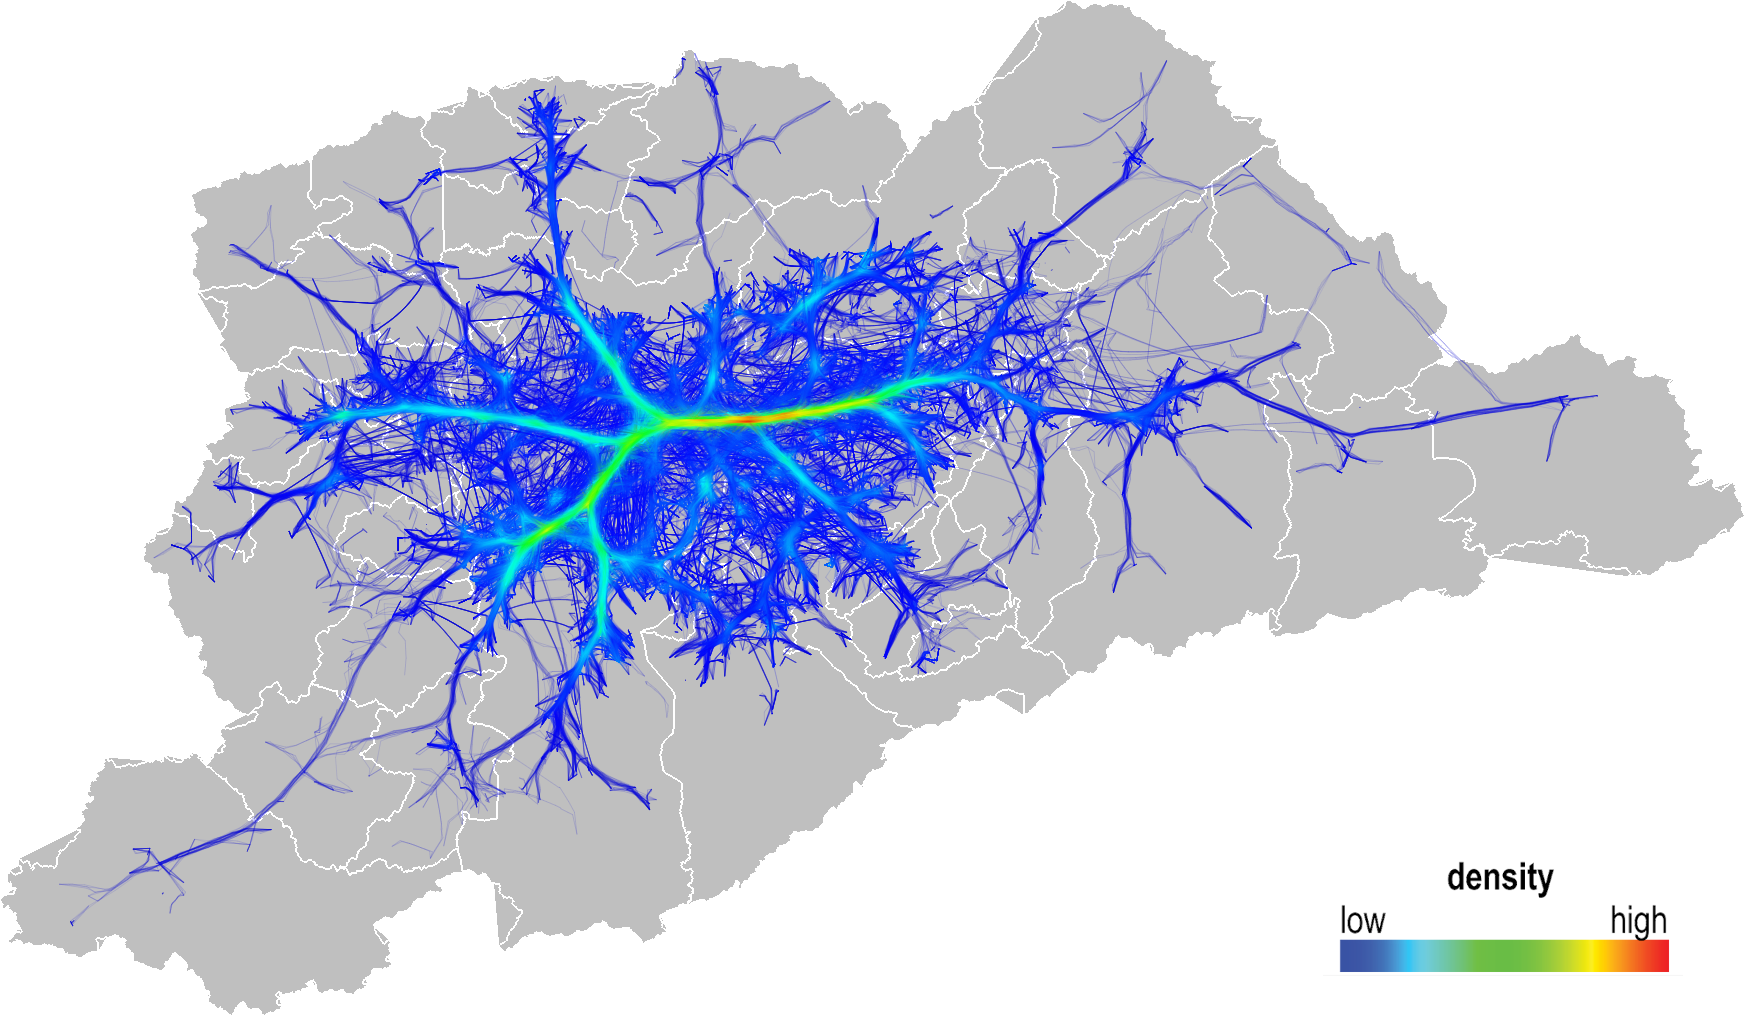
\includegraphics[width=0.98\textwidth]{../figuras/5-class-c2.png}
  \caption{Densidade das viagens da classe $C2$. \label{fig:becc-c2}}
\end{figure}

\begin{figure}[!htb]
  \centering
  \captionsetup{justification=centering}
  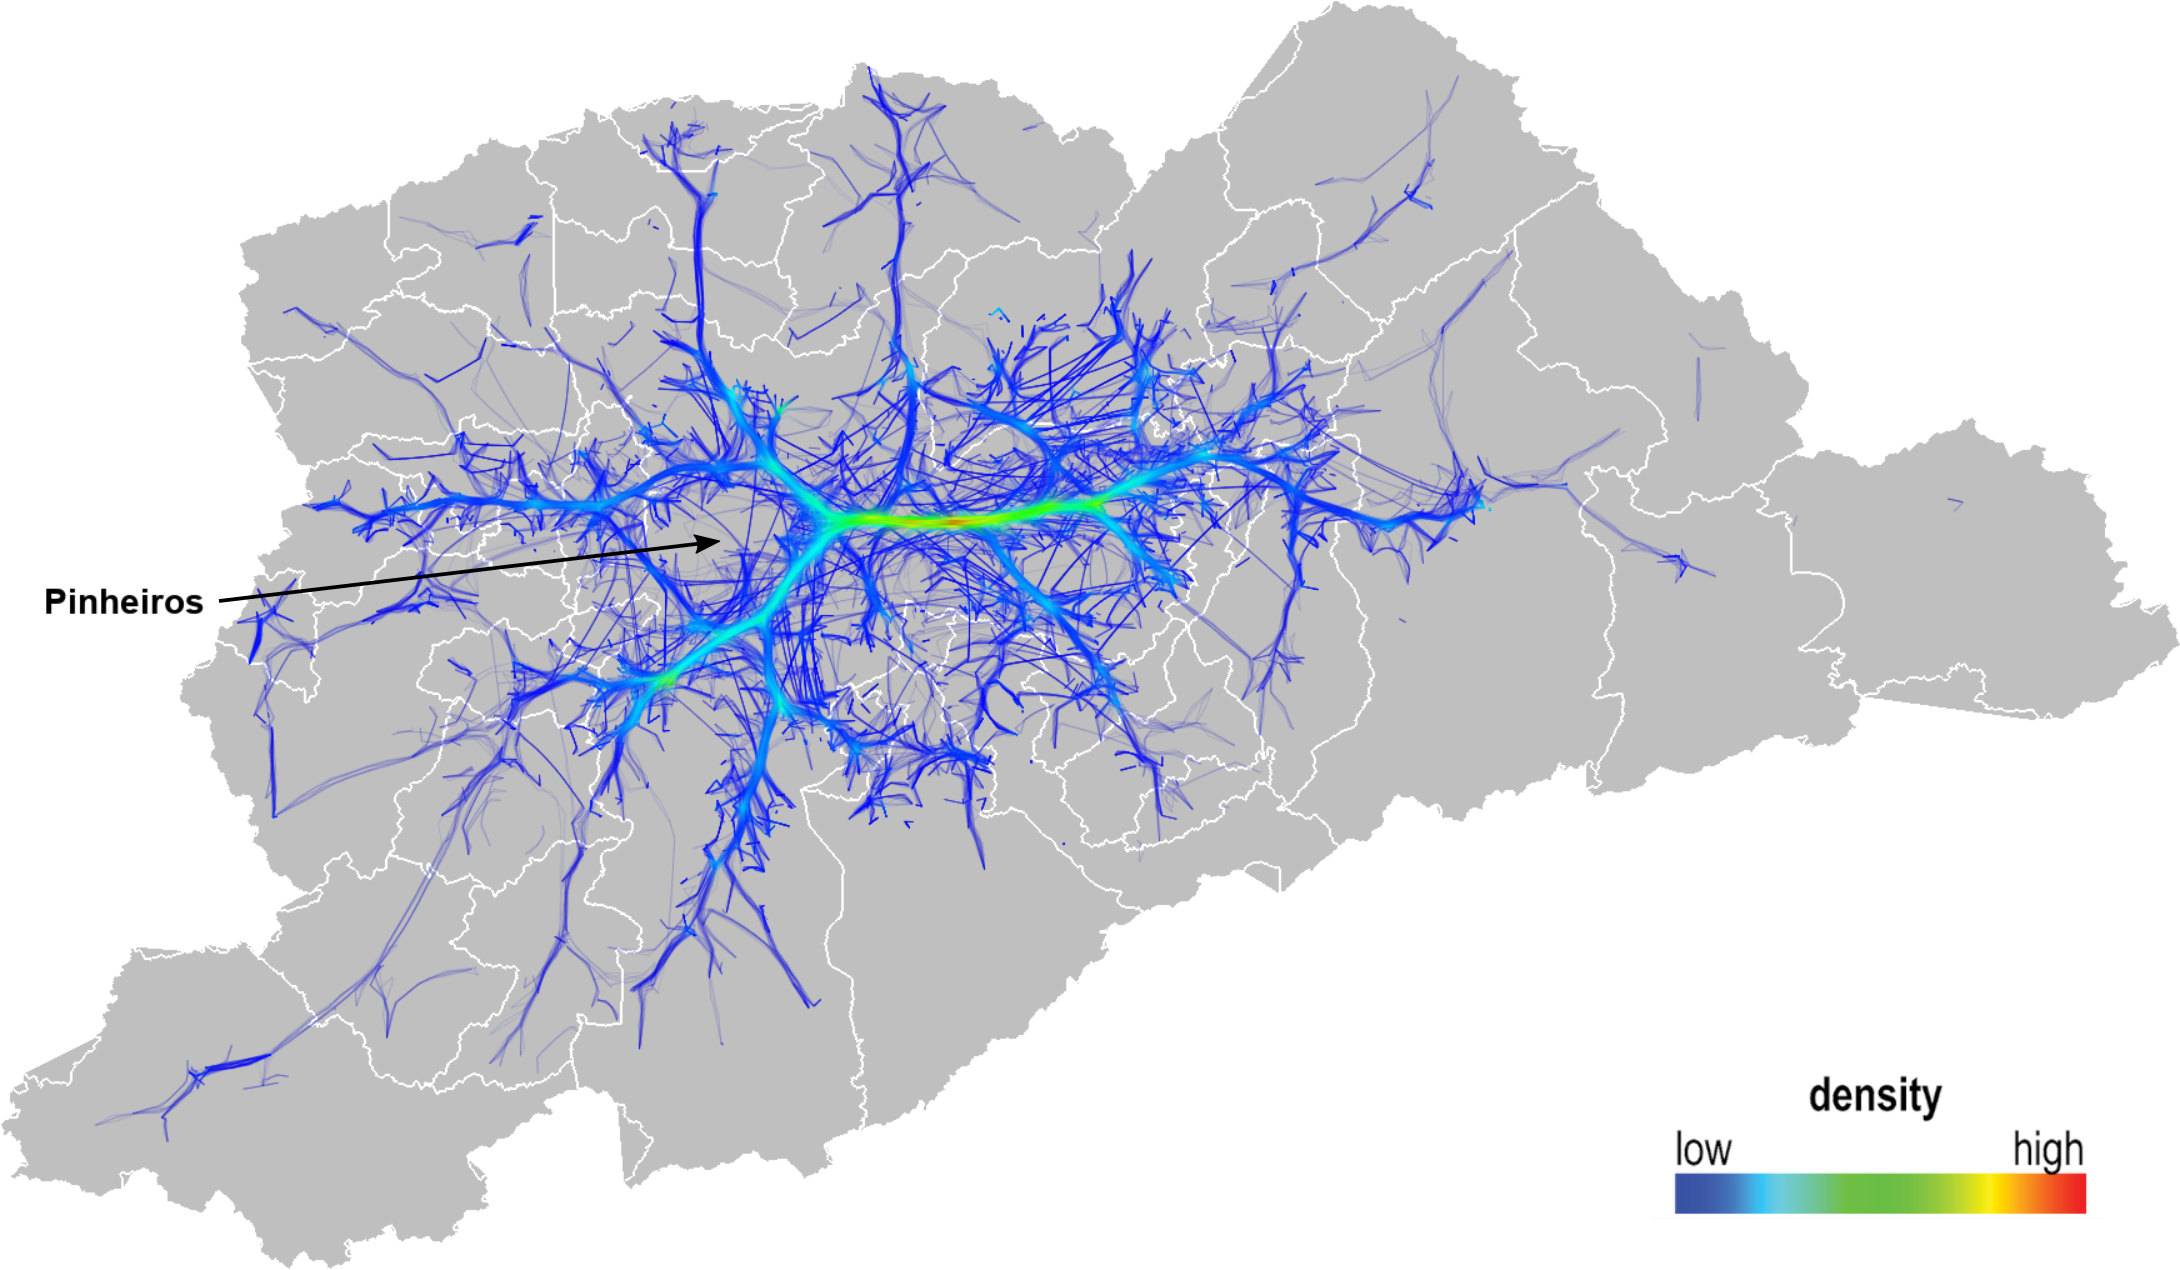
\includegraphics[width=0.98\textwidth]{../figuras/6-class-d-e.png}
  \caption{Densidade das viagens da classe $D$-$E$. \label{fig:becc-d-e}}
\end{figure}

Quando comparamos todos os mapas do nível $A$ ao $D-E$
(Figuras~\ref{fig:becc-a}~to~\ref{fig:becc-d-e}), vemos que os fluxos mais
densos (em vermelho) tendem a se deslocar do centro da capital para a região
leste da cidade. A concentração de fluxos de alta densidade está se espalhando
cada vez mais do centro para as regiões periféricas da RMSP. Mesmo os fluxos
menos densos também se espalham pela RMSP. No entanto, o mapa $D-E$ mostra que
esses fluxos diminuem consideravelmente (podemos ver pelas linhas menos densas)
para essas classes sociais. Isso pode indicar que os cidadãos de baixa renda
têm menos acesso ao sistema de mobilidade urbana. Com isso, essas pessoas teriam
menos acesso aos serviços sociais, educacionais, de saúde e culturais da RMSP,
uma vez que esses recursos estão concentrados nas regiões centrais das cidades.
É importante notar que essas regiões centrais também têm mais oportunidades de
emprego. Olhando o mapa $D-E$, podemos ver um notável espaço vazio no centro
oeste da capital. Essa região (distrito de Pinheiros) concentra um grande número
de empregos relacionados à tecnologia da informação e serviços financeiros, o
que requer trabalhadores com níveis de escolaridade alto e médio. Assim, o mapa
mostra que os cidadãos de baixa renda não estão indo para aquela região, o que
reflete a desigualdade de oportunidades que esses cidadãos enfrentam.

\section{Mobilidade de jovens estudantes de diferentes classes sociais}
\label{sec:students}

Um outro uso do \emph{bundling} que fizemos em nosso estudo de visualização de padrões de
mobilidade foi para comparar as viagens de estudantes de diferentes classes
sociais. Para isso, filtramos viagens de indivíduos com idades entre 6 e 18 anos
cujo motivo do deslocamento é o estudo. Então, nós os dividimos em dois grupos,
de alta a moderada renda, que inclui os níveis CCEB $A$, $B1$, $B2$ e $C1$; e os
de baixa renda, que incluem os níveis $C2$ e $D$ - $E$. As
figuras~\ref{fig:students-high}~e~\ref{fig:students-low} mostram os mapas de
densidade para ambos os grupos.

\begin{figure}[!htb]
  \centering
  \captionsetup{justification=centering}
  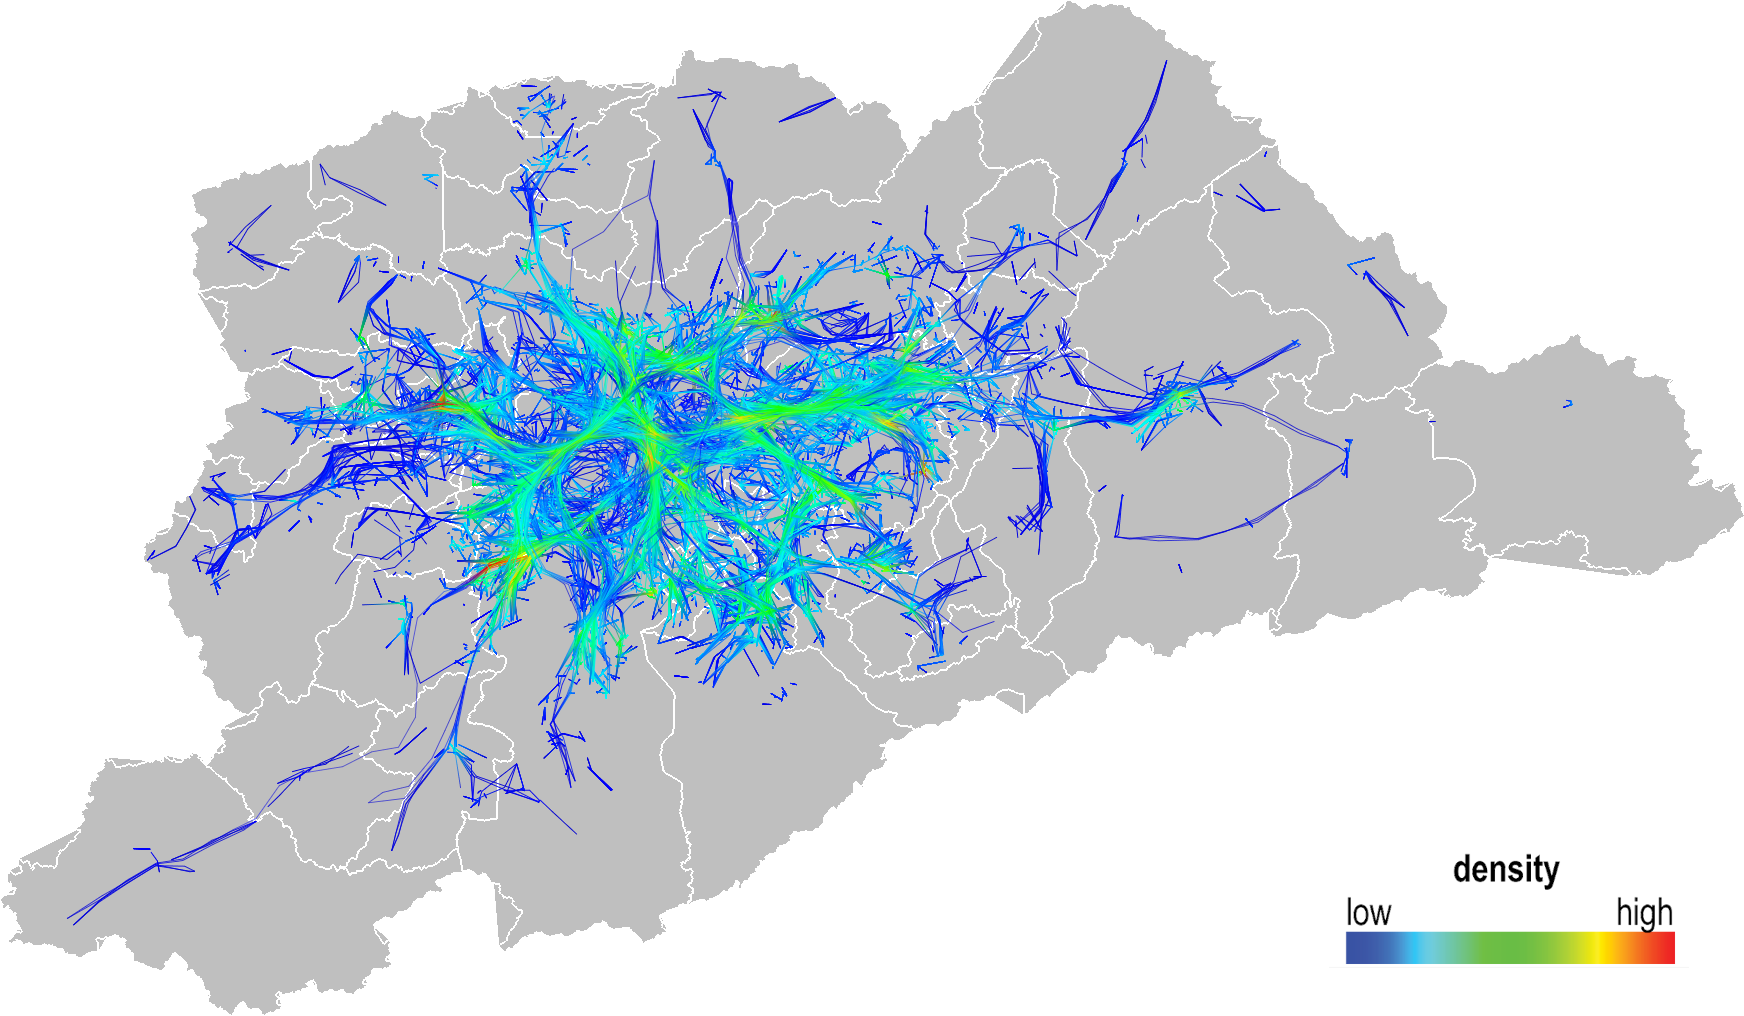
\includegraphics[width=0.98\textwidth]{../figuras/high-income-density-leg.png}
  \caption{Densidade das viagens de estudantes de alta renda. \label{fig:students-high}}
\end{figure}
\vspace*{\floatsep}
\begin{figure}[!htb]
  \centering
  \captionsetup{justification=centering}
  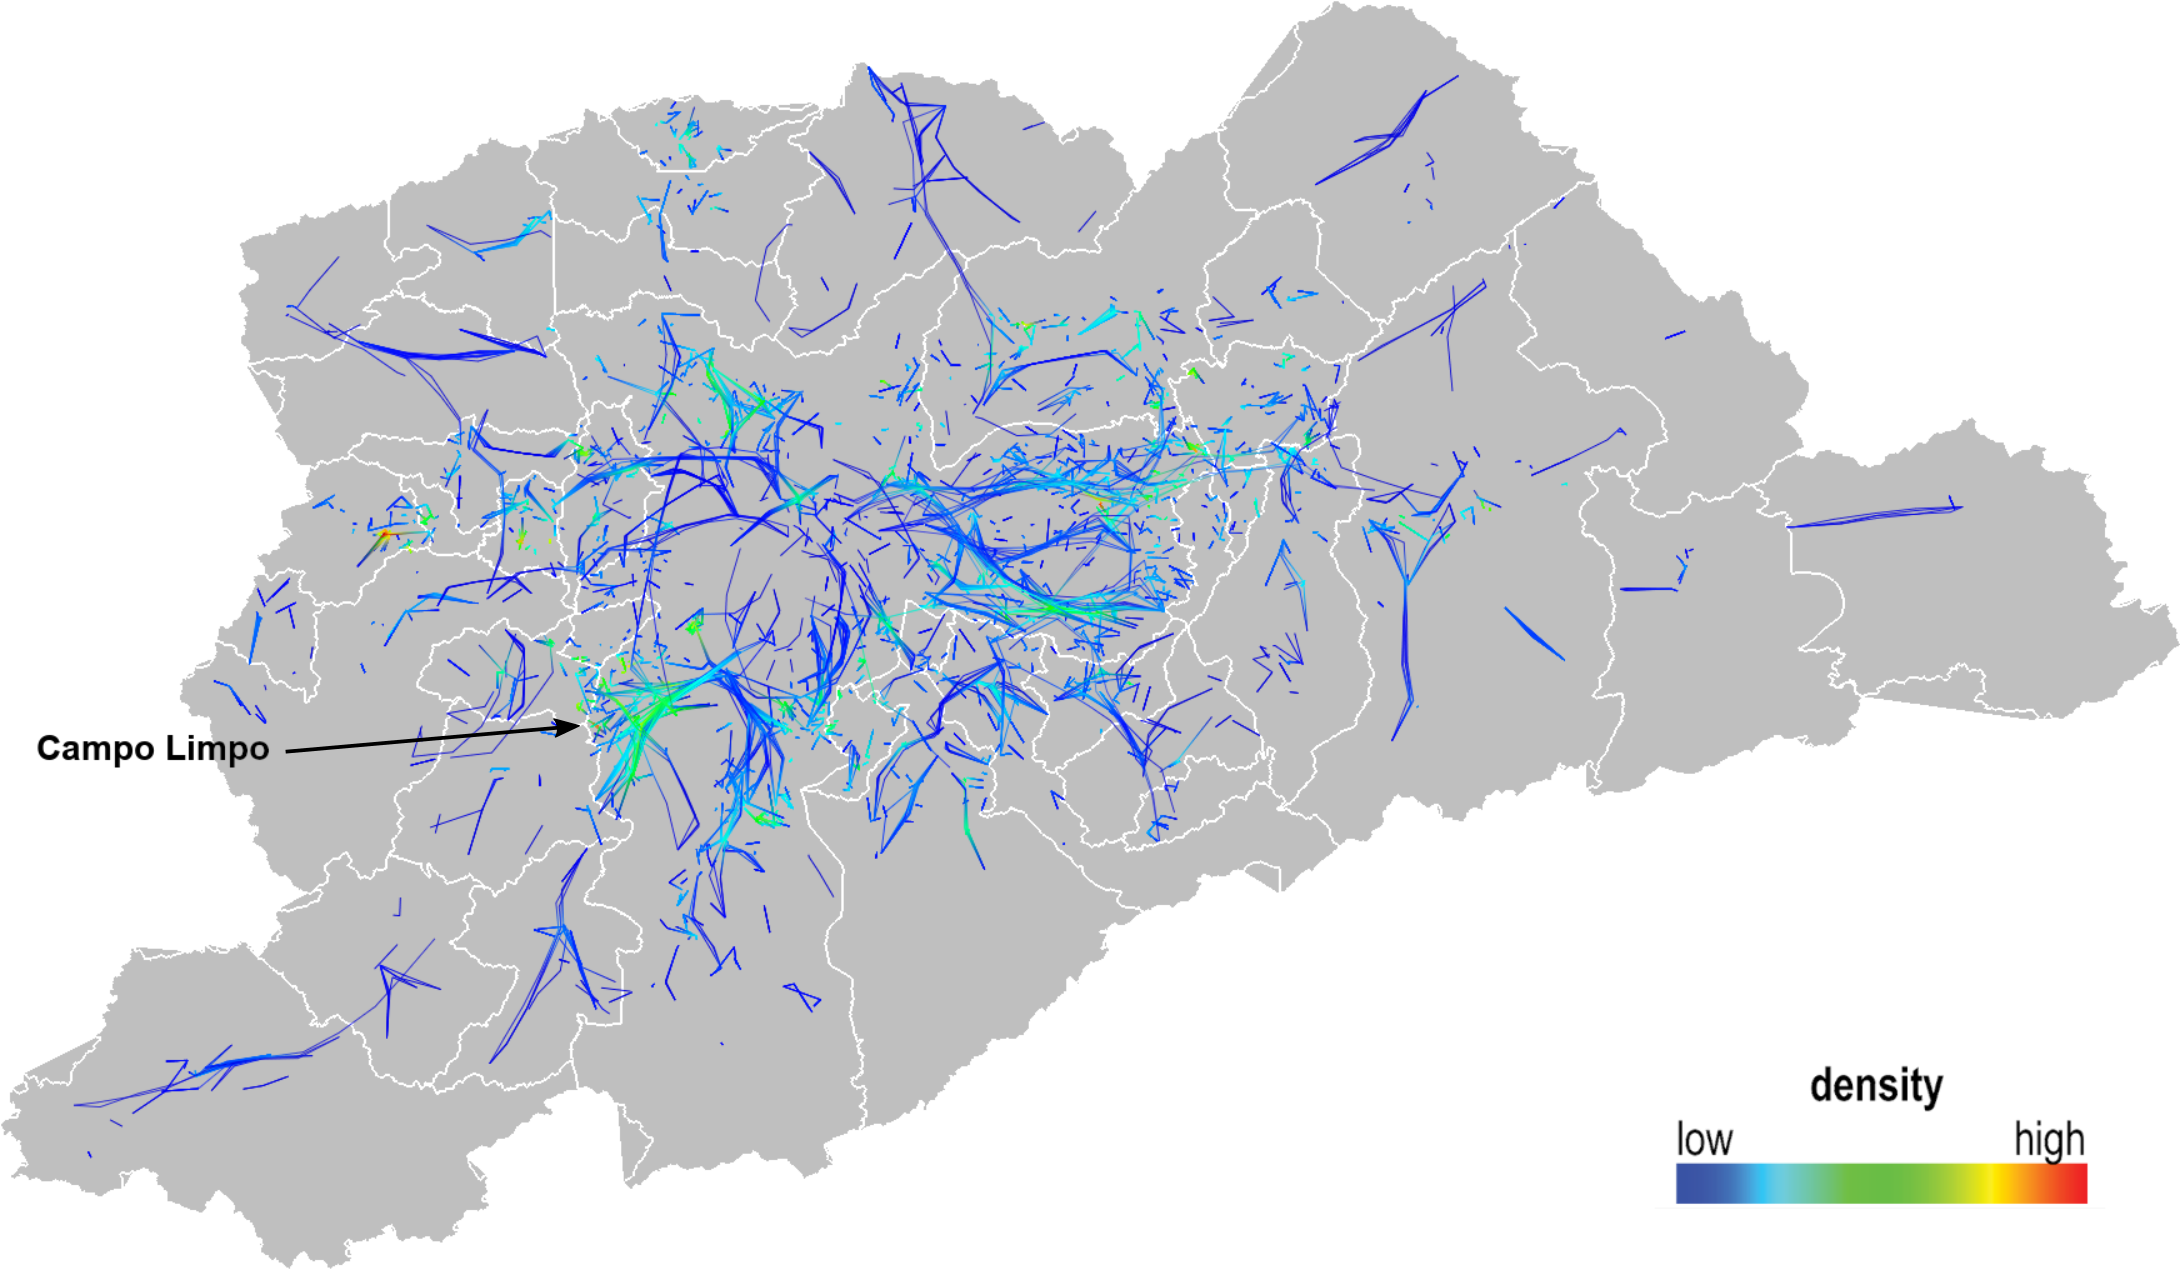
\includegraphics[width=0.98\textwidth]{../figuras/low-income-density-leg.png}
  \caption{Densidade das viagens de estudantes de baixa renda. \label{fig:students-low}}
\end{figure}

Podemos ver no mapa da Figura~\ref{fig:students-high} que a densidade dos fluxos
do grupo de alunos de alta a moderada renda se mostram muito mais densos e
espalhados pela a região central da RMSP. Esta parte da RMSP concentra a maioria
das escolas particulares, universidades e faculdades. Já o mapa de densidade de
alunos de baixa renda (Figura~\ref{fig:students-low}) mostra uma mobilidade bem
mais limitada em comparação com os alunos de alta renda, com alguns fluxos
interligados ao centro da capital, mas a maioria dos fluxos densos dessa classe
estão mais presentes nas periferias da capital e também nas cidades vizinhas.
Apesar das diferenças, podemos ver que há concentração dos dois grupos na região
sudoeste, onde ficam os bairros do distrito de Campo Limpo.

Podemos observar que há muito mais trilhas para os alunos de alta renda
(Figura~\ref{fig: students-high}) do que para alunos de baixa renda
(Figura~\ref{fig:students-low}). Os estudantes de renda alta também viajam
grandes distâncias para estudar, o que indica que podem escolher com mais
flexibilidade onde estudar. Este fato é corroborado por estudos de mobilidade
urbana que indicam que pessoas com melhores condições financeiras têm mais
mobilidade do que aquelas com condições mais precárias, como em \citet{carruthers2005,
lucas2016}.

Vale ressaltar que as escolas de ensino públicas   da RMSP estão distribuídas pela região
central e periférica das cidades. Em geral, o sistema público busca alocar as
matrículas dos alunos nessas escolas de acordo com a proximidade de suas
residências. Assim, eles não precisam viajar longas distâncias para chegar às
suas escolas. Além disso, as escolas públicas apresentam desempenho educacional
inferior ao das escolas particulares de São Paulo. Assim, cidadãos com melhores
condições financeiras costumam colocar seus filhos em escolas particulares,
padrão que se inverte no ensino superior.

A escassez de fluxos de alunos de baixa renda levanta questionamentos. Ela pode
ser uma indicação de que essa classe da população não tem oportunidades iguais
de estudo. Também não costumam ir para a região central da cidade e, portanto,
têm menos acesso a universidades e faculdades complementares. Essa desigualdade
de oportunidades provavelmente afetará os empregos e as condições econômicas
desses alunos.

\section{Direção das viagens nos horários de pico}
\label{sec:peak-hours}

Conforme mostramos anteriormente na Figura~\ref{fig:trips_by_hour} da
Seção~\ref{sec:pesquisa-od}, distribuição das viagens por hora do dia tem dois
picos principais, entre 6 e 9h e entre 17 e 20h. No entanto, essa tabela
agregada não fornece informações sobre como os padrões de mobilidade nos
horários de pico podem ser diferentes. Para visualizar esses dados aplicamos o
\emph{bundling} no conjunto de dados e então aplicamos um filtro que para
alterar a transparência das viagens fora do horário selecionado. Codificamos a
direção a das viagens em cores, similar ao apresentado na
Figura~\ref{fig:attributes-direction}, da Seção~\ref{sec:length-direction}.

\begin{figure}[!htb]
  \centering
  \captionsetup{justification=centering}
  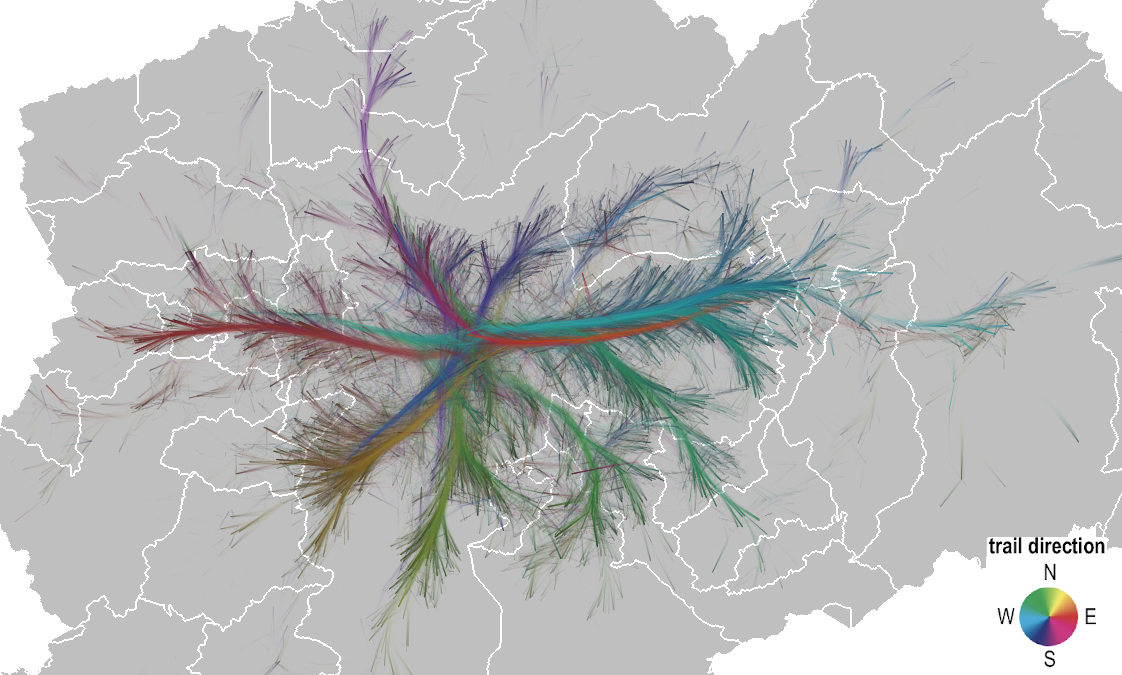
\includegraphics[width=0.98\textwidth]{../figuras/peak-hours-6h-to-9h-direction-leg.png}
  \caption{Direção das viagens entre 6 e 9 da manhã. \label{fig:peak-hours-6h-9h}}
\end{figure}
\vspace*{\floatsep}
\begin{figure}[!htb]
  \centering
  \captionsetup{justification=centering}
  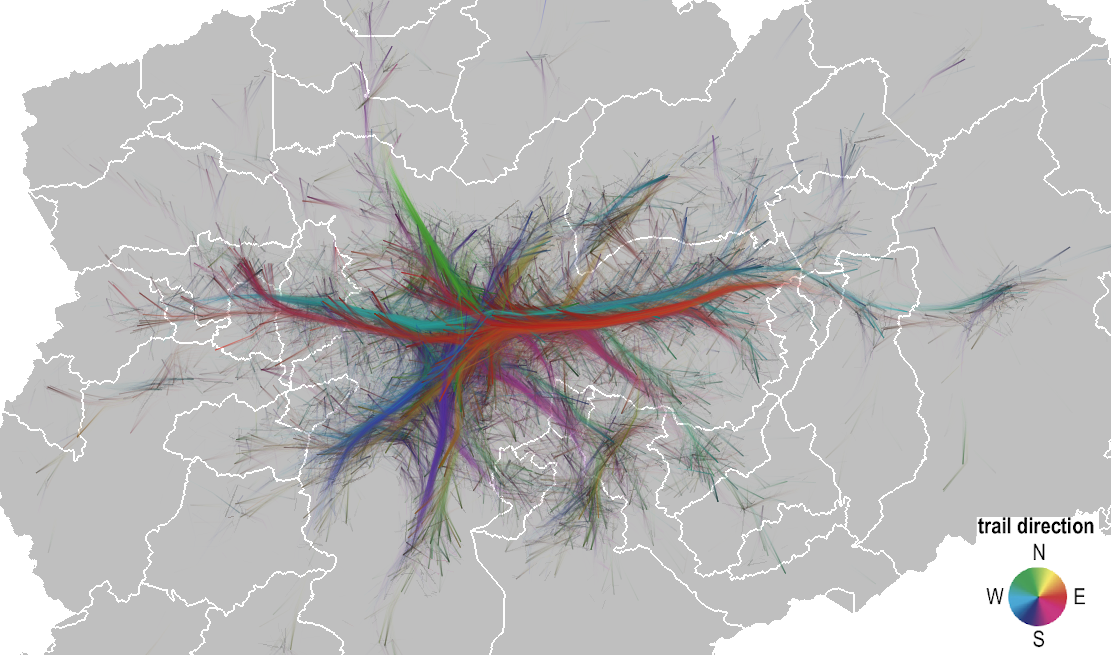
\includegraphics[width=0.98\textwidth]{../figuras/peak-hours-17h-to-20h-direction-leg.png}
  \caption{Direção das viagens entre 17 e 20h. \label{fig:peak-hours-17h-20h}}
\end{figure}

Comparando as horas de pico, podemos ver que os fluxos matinais indo para o
centro da RMSP (Figura~\ref{fig:peak-hours-6h-9h}, fluxo ciano vindo do leste)
são geralmente mais densos e mais longos do que os fluxos vindos do Centro RMSP
durante o pico da tarde/noite (Figura~\ref{fig:peak-hours-17h-20h}, fluxo
vermelho). Isso sugere que na manhã as pessoas têm um comportamento na ida ao
trabalho, ao passo que esse fluxo se distribui de maneira diferente na volta
para casa, possivelmente se designando para outros destinos (como escolas ou
academia) no período da tarde/noite. Um recurso interessante para esse tipo de
visualização é a separação das trajetórias em direções opostas alterando-se
diretamente o algoritmo de \emph{bundling}, como sugere \citet{adeb}. Em teoria,
sua técnica seria capaz de gerar agrupamentos mais nítidos levando em
consideração esse atributo. Porém, por questões de limite tempo e escopo deste
trabalho, não nos aprofundamos nesse tópico.

\section{Densidade das viagens por modo de transporte}
\label{sec:mode}

Um outro interessante atributo presente nos dados da pesquisa OD17 é o modo de
transporte. Comparamos então padrões de fluxo para quatro modos de transporte
diferentes: pedestres, bicicletas, carros e metrô. Nas
figuras~\ref{fig:mode-pedestrian}~até~\ref{fig:mode-subway} utilizamos o
\emph{bundling} para visualizar a densidade dos fluxos de cada um dos tipos de
transporte. Diferentemente do que apresentamos na seção~\ref{sec:coloring}, onde
aplicamos \emph{bundling} em todo o conjunto de dados e utilizamos filtros para
selecionar categorias de transporte de interesse, aqui utilizamos a estratégia de
particionamento para visualizar cada conjunto separadamente. Com isso damos
ênfase às características de cada subconjunto em específico, já que o
mapa de densidade é calculado com os valores daquela única classe de atributos.
 
\begin{figure}[!htb]
  \centering
  \captionsetup{justification=centering}
  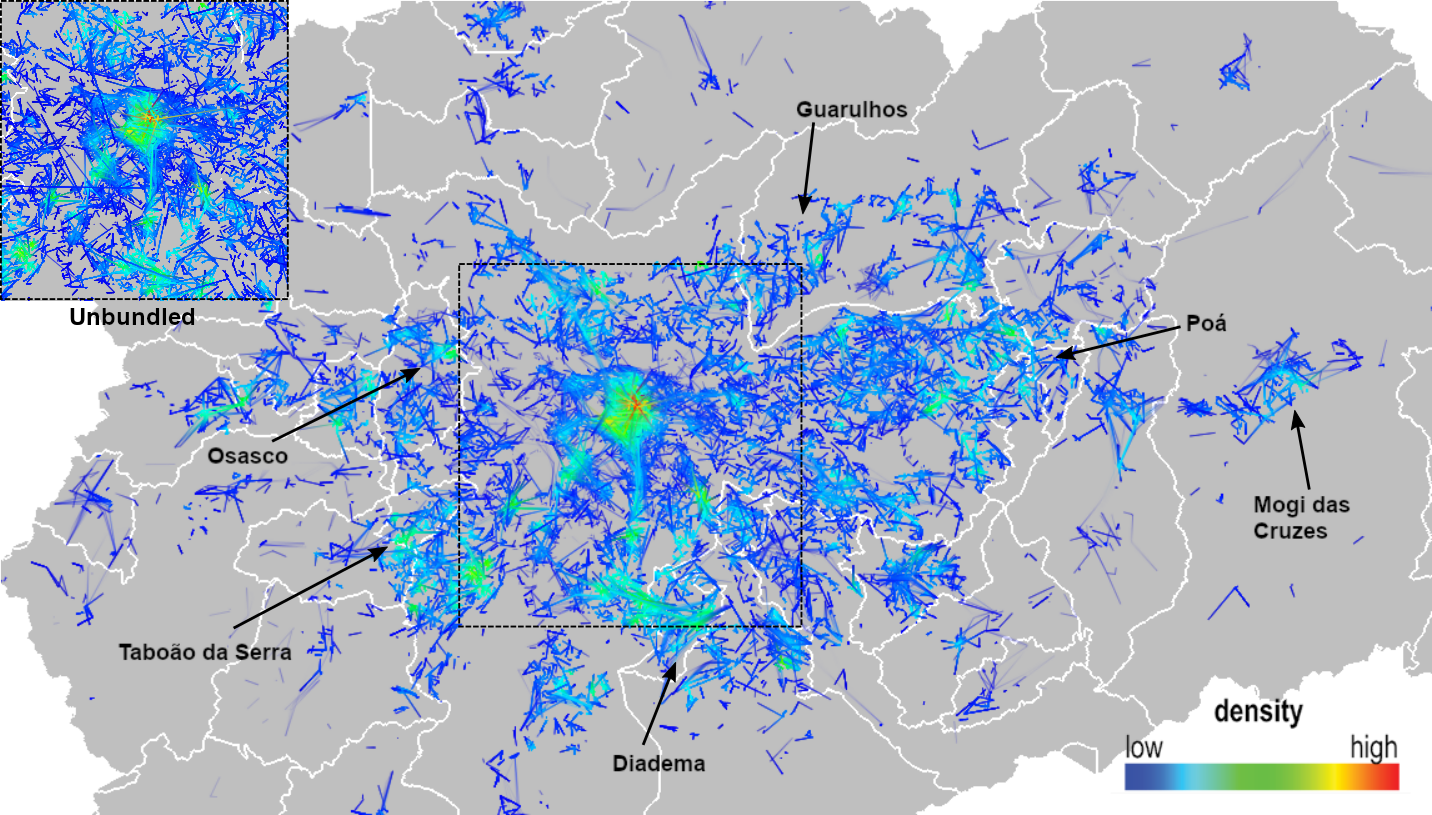
\includegraphics[width=0.98\textwidth]{../figuras/mode-pedestrian-density-leg.png}
  \caption{Densidade das viagens de pedestres. \label{fig:mode-pedestrian}}
\end{figure}

\begin{figure}[!htb]
  \centering
  \captionsetup{justification=centering}
  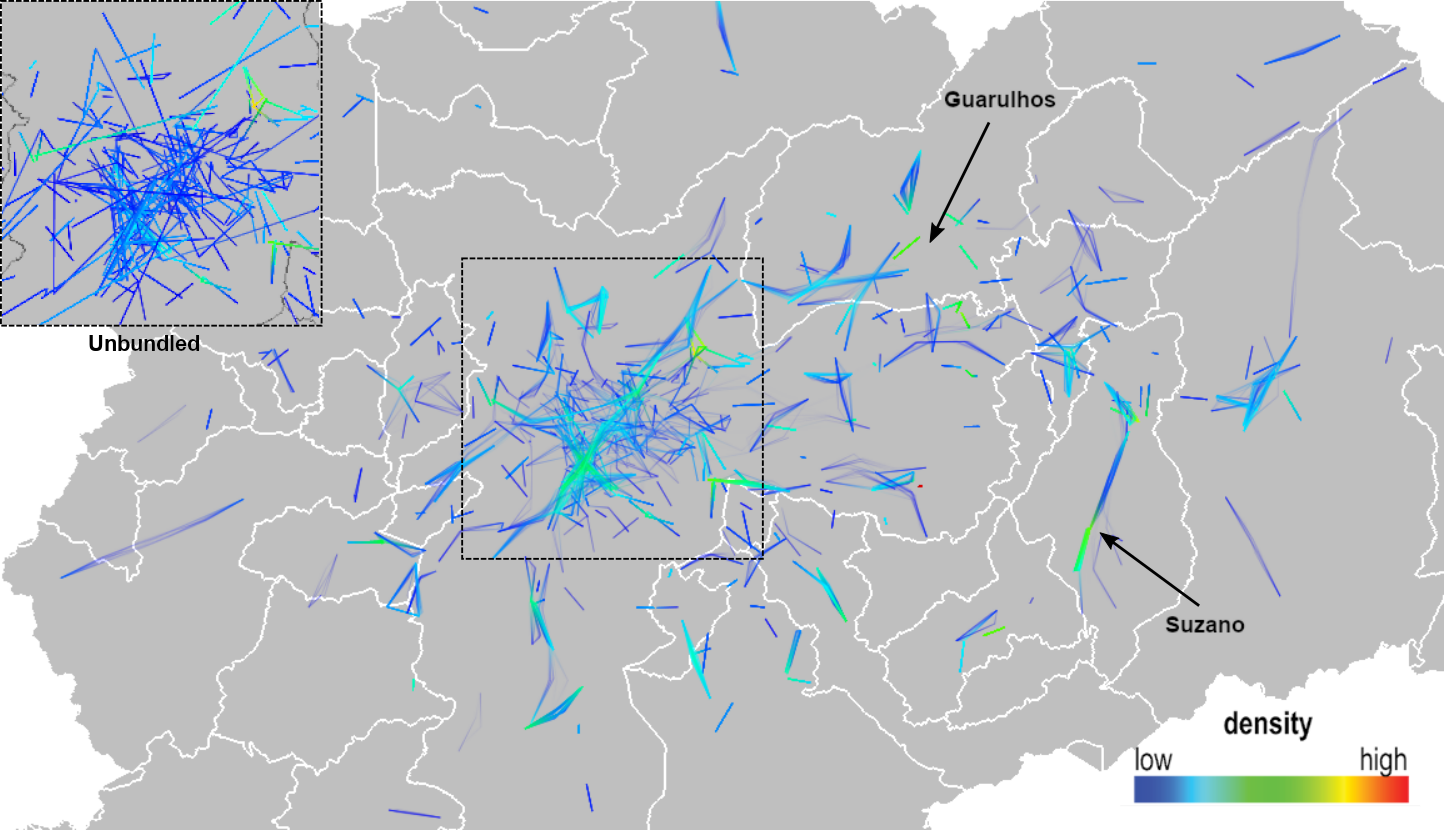
\includegraphics[width=0.98\textwidth]{../figuras/mode-bike-density-leg.png}
  \caption{Densidade das viagens de bicicleta \label{fig:mode-bike}}
\end{figure}

\begin{figure}[!htb]
  \centering
  \captionsetup{justification=centering}
  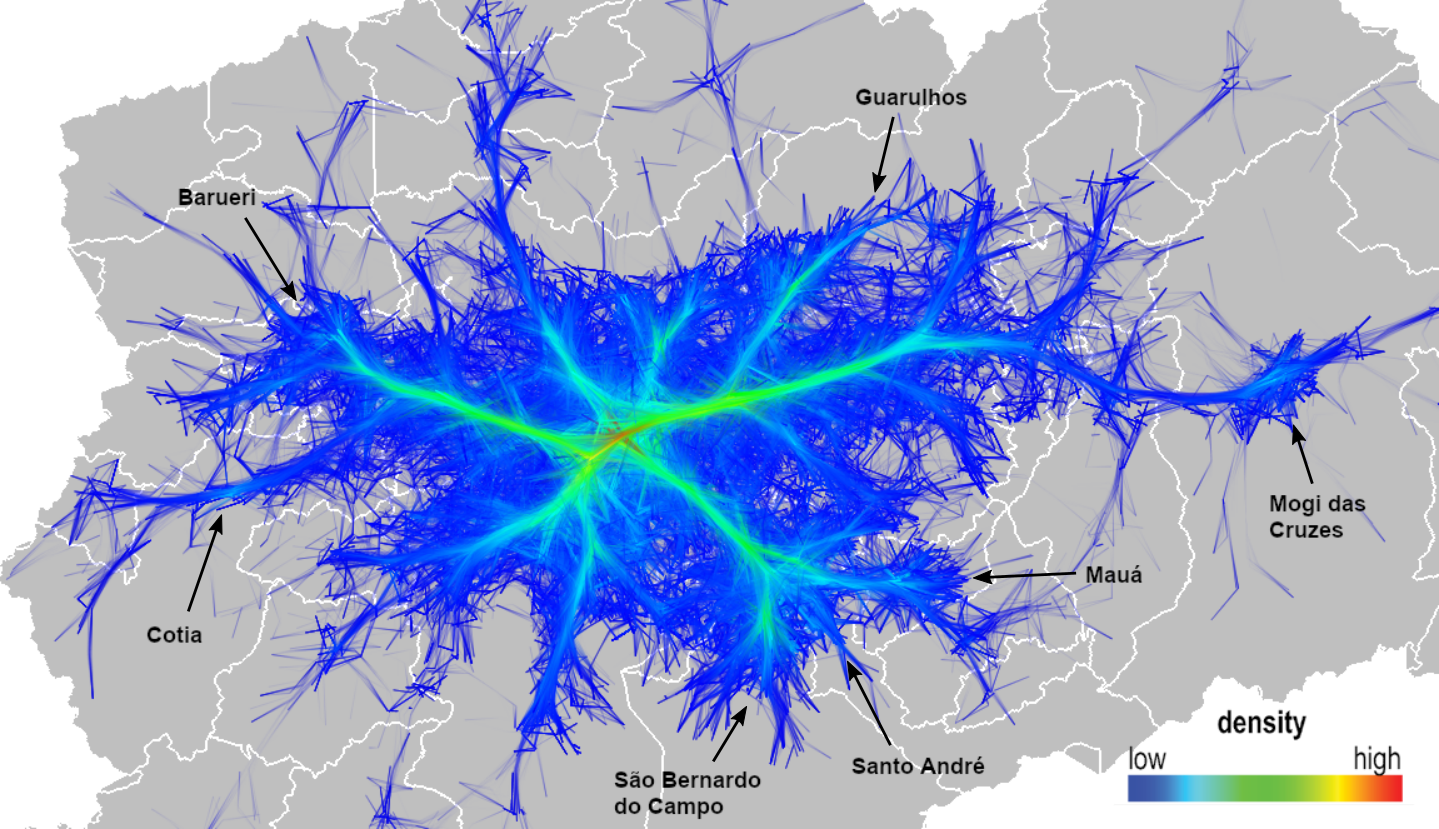
\includegraphics[width=0.98\textwidth]{../figuras/mode-car-density-leg.png}
  \caption{Densidade das viagens de carro. \label{fig:mode-car}}
\end{figure}

\begin{figure}[!htb]
  \centering
  \captionsetup{justification=centering}
  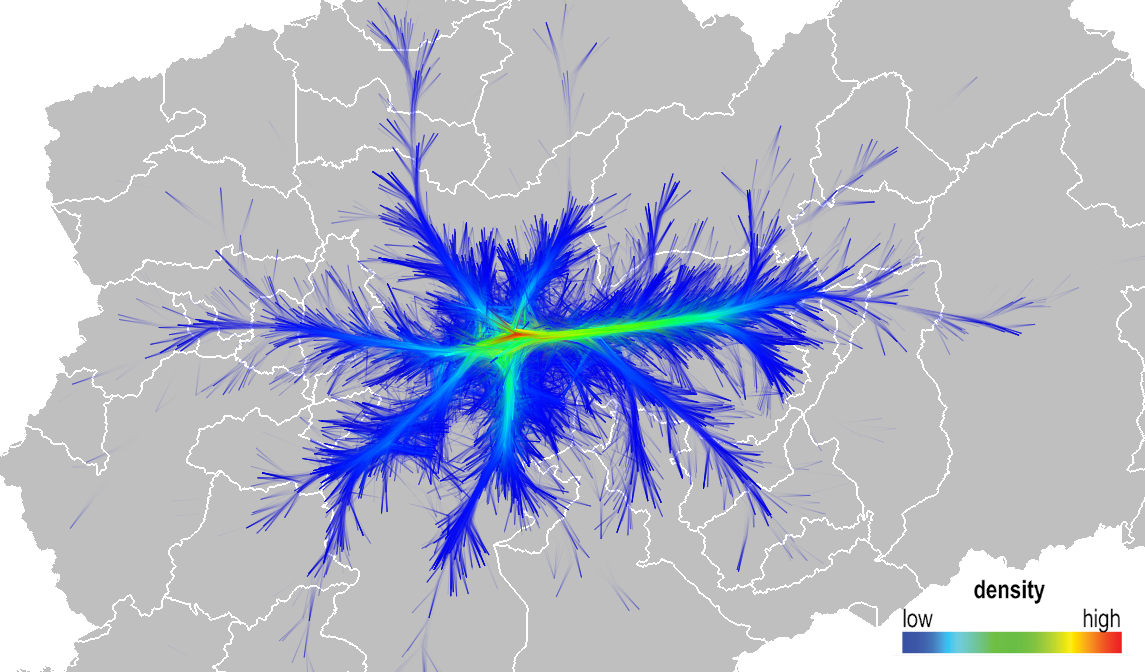
\includegraphics[width=0.98\textwidth]{../figuras/mode-subway-density-leg.png}
  \caption{Densidade das viagens de metrô e trem. \label{fig:mode-subway}}
\end{figure}

As viagens de pedestres (Figura~\ref{fig:mode-pedestrian}) formam várias
``ilhas'' de baixa densidade espalhadas pela RMSP, sendo a mais densa (em vermelho)
no centro da capital. A maioria das trilhas são curtas, o que
é esperado para pedestres. No entanto, vemos alguns \emph{bundles} mais longos se estendendo
entre o centro da capital e as regiões sul e norte da cidade. Alguns fluxos mais densos também
estão presentes nas cidades vizinhas de Diadema, Taboão da Serra, Osasco,
Guarulhos, Poá e Mogi das Cruzes. Examinando mais de perto, observamos que
os fluxos densos combinam geograficamente com áreas centrais das cidades e as áreas comerciais. Essas
informações podem ser úteis para localizar locais que possam merecer a atenção
dos governos locais para proporcionar melhorias aos pedestres.

Como a maioria das viagens de pedestres são curtas, a técnica de \emph{bundling}
forma poucos fluxos sobre a RMSP. Usar o \emph{bundling} para essas viagens
curtas resulta em alguns poucos fluxos de baixa densidade, o que é menos útil em
comparação com viagens longas. Em casos como este, pode não ser necessário usar
o \emph{bundling}. Na área superior esquerda da
Figura~\ref{fig:mode-pedestrian}, temos destacadas as viagens OD da área central da
cidade sem utilização do \emph{bundling}; podemos ver que são quase idênticas
aos resultados com \emph{bundling} aplicado.

Com uma média de menos de três quilômetros, as viagens de bicicleta
(Figura~\ref{fig:mode-bike}) exibem padrões semelhantes aos de pedestres.  Nessa
figura, vemos alguns fluxos estreitos na área central da capital. Existem também
alguns fluxos mais salientes no Nordeste da capital e nas cidades vizinhas de
Suzano e Guarulhos. No entanto, comparando a Figura~\ref{fig:mode-bike} com
todos os outros meios de transporte, vemos imediatamente que as viagens de
bicicleta são de longe as menos numerosas e exibem um padrão muito mais esparso,
com poucos caminhos em forma de estrela onde muitas trajetórias se encontram.
Isso sugere que a infraestrutura de ciclismo em 2017 ainda era bastante limitada e fragmentada.
No canto superior esquerdo da Figura~\ref{fig:mode-bike} também mostramos
as viagens sem utilização do \emph{bundling}.

As viagens de carro (Figura~\ref{fig:mode-car}) mostram um padrão
semelhante ao que exibe todo o conjunto de dados, (ver Figura~\ref{fig:bundled-graph-density}).
Para começar, isso indica que os carros são a forma
dominante de transporte na RMSP, respondendo pelos principais padrões de
tráfego. Os fluxos de maior densidade ocorrem no centro da capital. Podemos observar diversos
fluxos de alta densidade ligando o Centro às demais regiões da capital, e também
indo e vindo das cidades de Guarulhos, Barueri, Cotia, São Bernardo do Campo,
Santo André, Mauá, e Mogi das Cruzes. Em comparação com todos os outros
modos de transporte, os carros mostram um padrão muito mais ``espalhado'' que
cobre áreas muito grandes, indicando que os carros são o modo de transporte
predominante na maioria das regiões da RMSP.

Por fim, as viagens de metrô e trem (Figura~\ref{fig:mode-subway}) apresentam um
forte padrão em forma de estrela, com fluxos de alta densidade que ligam a
capital às cidades vizinhas, devido à integração dos dois sistemas (vide
Seção~\ref{sec:trail-overlap}). Comparado aos outros modos de transporte, o
sistema de transporte de trilhos apresenta uma estrutura de padrão de viagem
mais clara e simples.

\section{Visualização por motivo da viagem}
\label{sec:dist_reasons}
Um outro atributo da pesquisa OD 17 que também achamos interessante em nossa
análise foi o motivo das viagens feitas. Observar a mobilidade urbana sobre essa
informação o pode revelar padrões comportamentais interessantes da população. A
seguir, estudamos as distâncias das viagens feitas por diferentes motivos, e que
tipos de padrões elas exibem. Para isso, criamos visualizações a partir dos
dados OD17 particionados por trabalho, saúde, educação e compras. As
figuras~\ref{fig:reason-work}~a~\ref{fig:reason-shopping} mostram os resultados.

As viagens de trabalho (Figura~\ref{fig:reason-work}) são geralmente mais longas
do que as outras razões de viagens e também cobrem uma área maior. Curiosamente, as viagens mais longas, entre o
lado leste e o centro da cidade (feixe vermelho), são um padrão semelhante às
viagens mais longas para saúde e educação. As viagens por motivos de saúde
(Figura~\ref{fig:reason-health}) são mais esparsas do que as relacionadas com o
trabalho e também apresentam um padrão mais estrelado, com longos fluxos
conectando-se à área central. Argumentamos que isso pode indicar que as regiões
periféricas não são bem servidas por serviços de saúde. As viagens por motivos
de estudo (Figura~\ref{fig:reason-education}) apresentam as maiores distâncias
entre as regiões Nordeste e Oeste da RMSP. Seu padrão apresenta ser algo
intermediário entre as viagens de trabalho e saúde. Curiosamente, as viagens
educacionais mostram várias ``voltas'' no centro da RMSP. Finalmente, as viagens
de compras (Figura~\ref{fig:reason-shopping}) mostram os padrões menos densos e,
em geral, também os mais curtos, mas com algumas exceções como o feixe vermelho
(importante) conectando o centro ao nordeste. Isso indica que, ao contrário da
saúde, educação e trabalho, os estabelecimentos comerciais (que na verdade são
da iniciativa privada) estão mais bem distribuídos na RMSP. Isso mostra que as
visualizações agregadas - como as feitas com \emph{bundling} - são úteis não
apenas quando mostram a \emph{presença} de certos dados, \emph{por exemplo}
viagens ligando regiões distantes; mas evidenciar a \emph{ausência} de padrões também
pode ser igualmente interessante.

\begin{figure}[!htb]
\centering
\captionsetup{justification=centering}
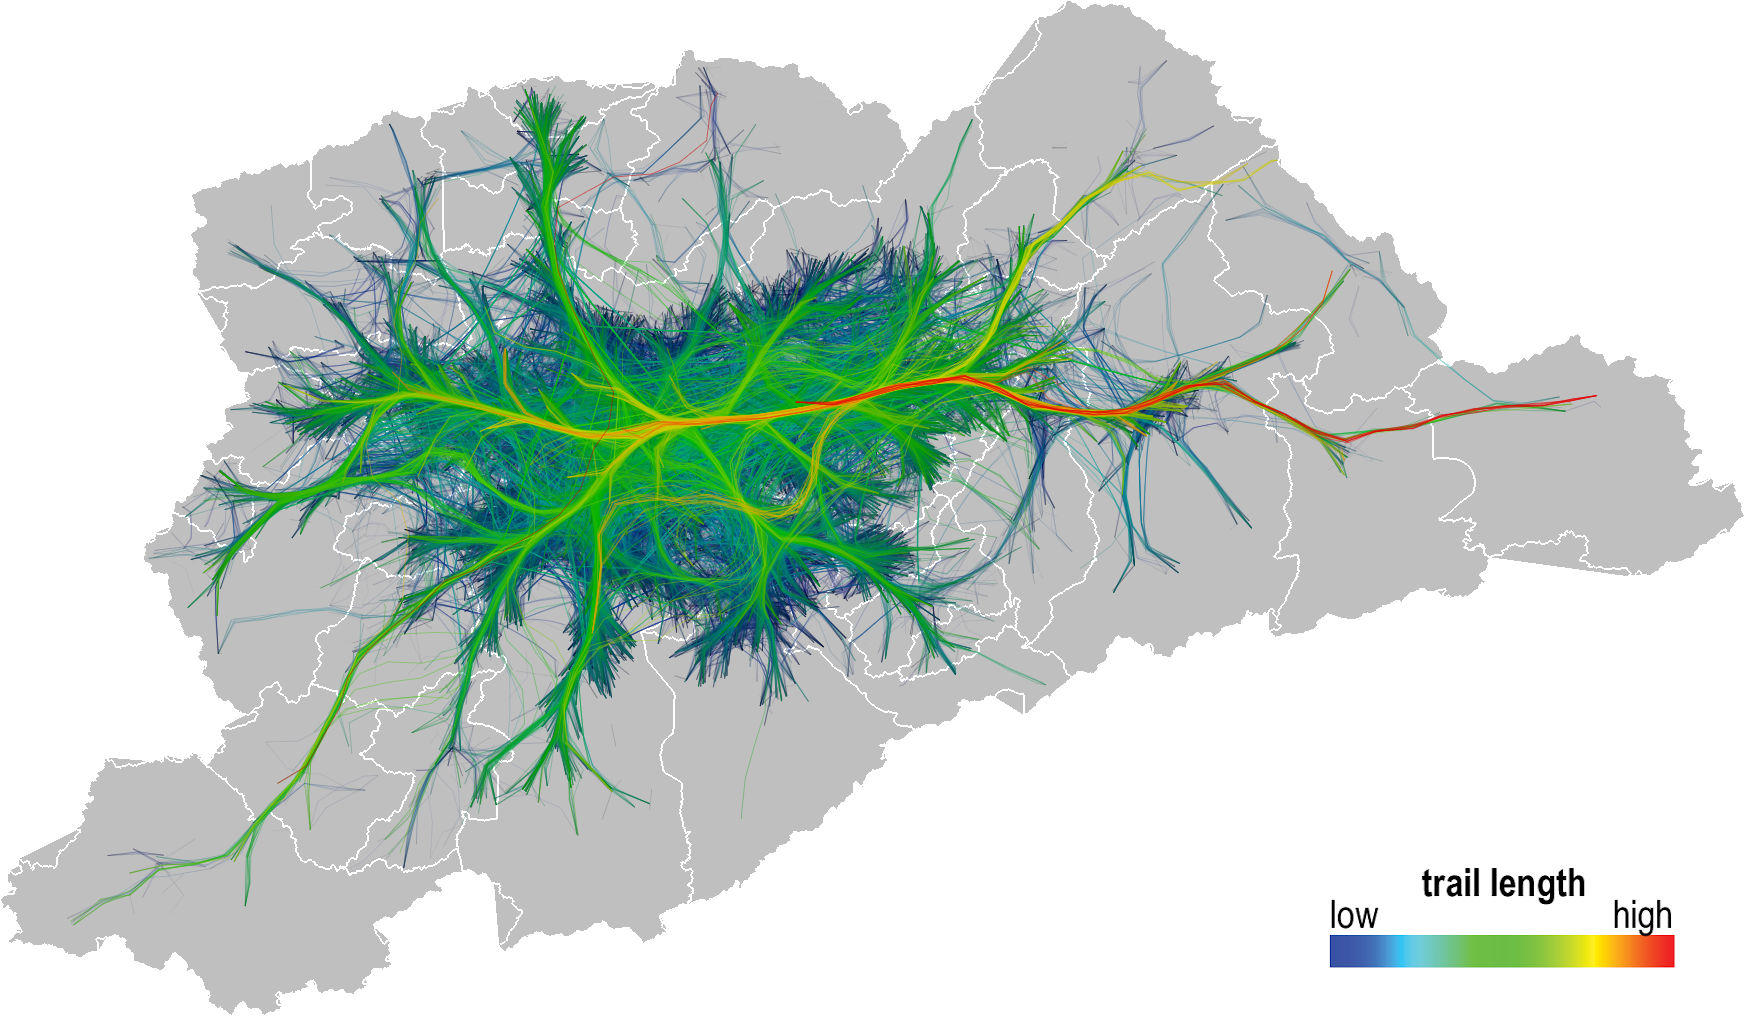
\includegraphics[width=0.98\textwidth]{../figuras/reason-work-leg.png}
\caption{Distâncias das viagens por motivo de trabalho.\label{fig:reason-work}}
\end{figure}
  
\begin{figure}[!htb]
\centering
\captionsetup{justification=centering}
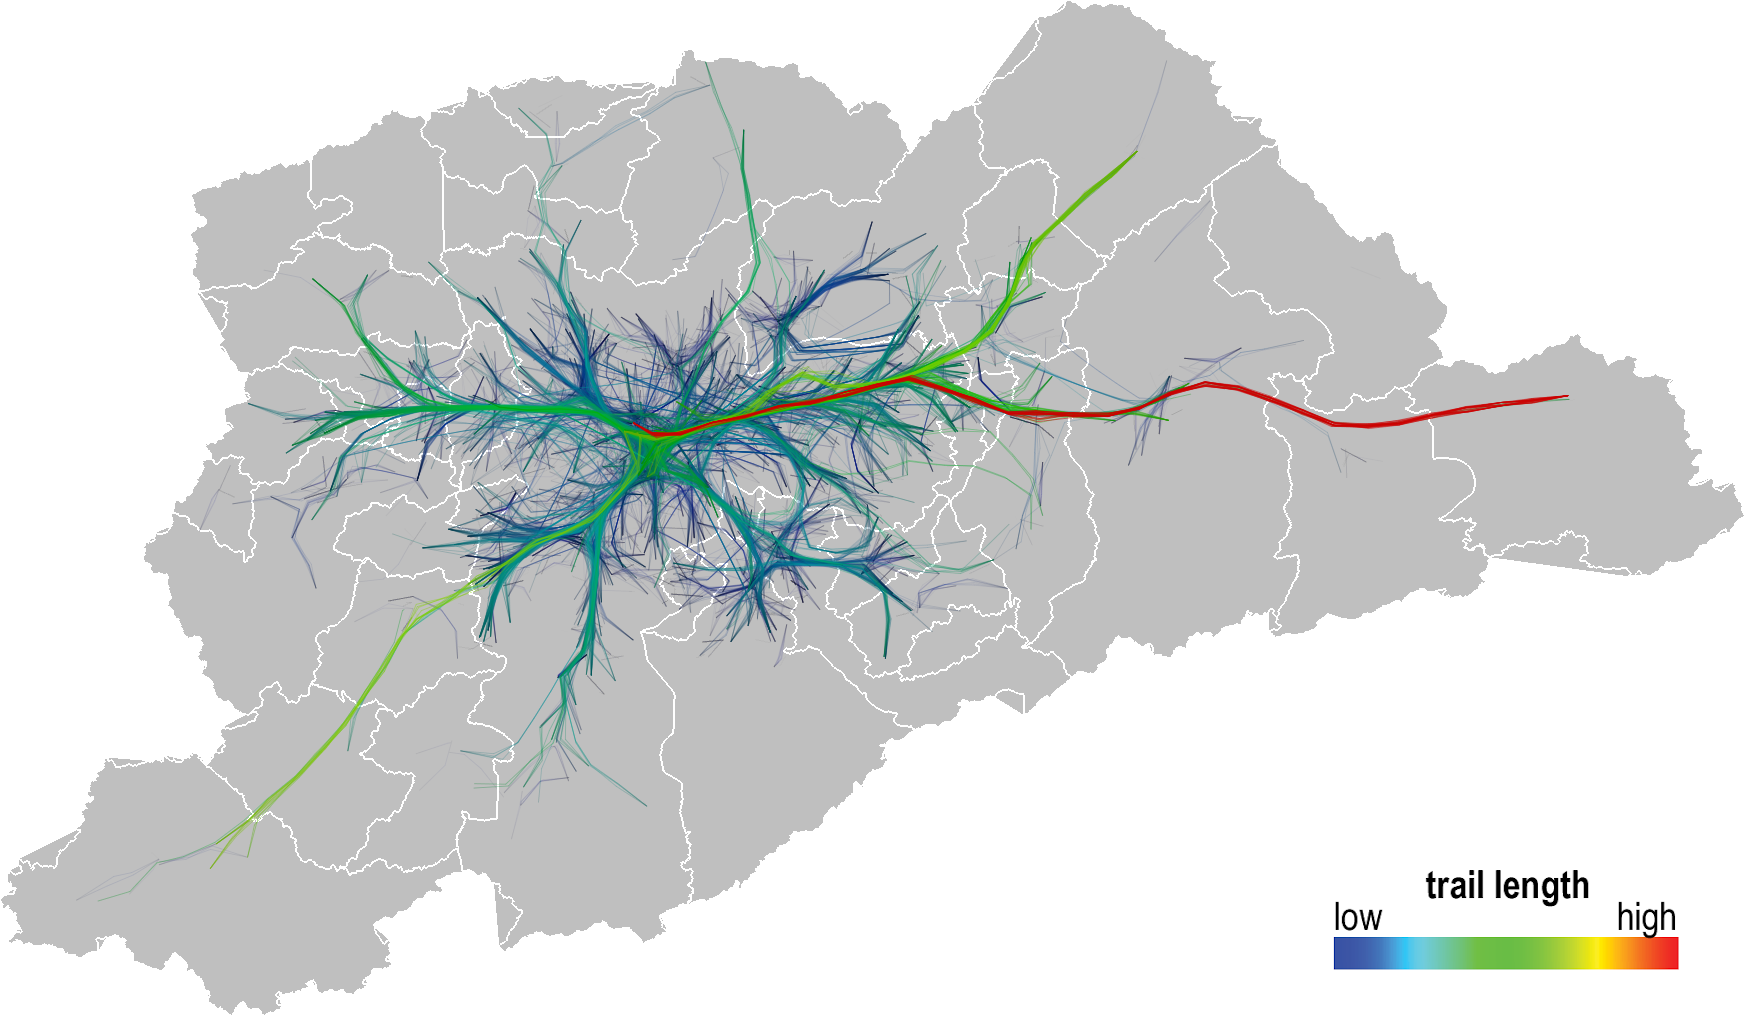
\includegraphics[width=0.98\textwidth]{../figuras/reason-health-leg.png}
\caption{Distâncias das viagens por motivo de saúde.\label{fig:reason-health}}
\end{figure}

\begin{figure}[!htb]
\centering
\captionsetup{justification=centering}
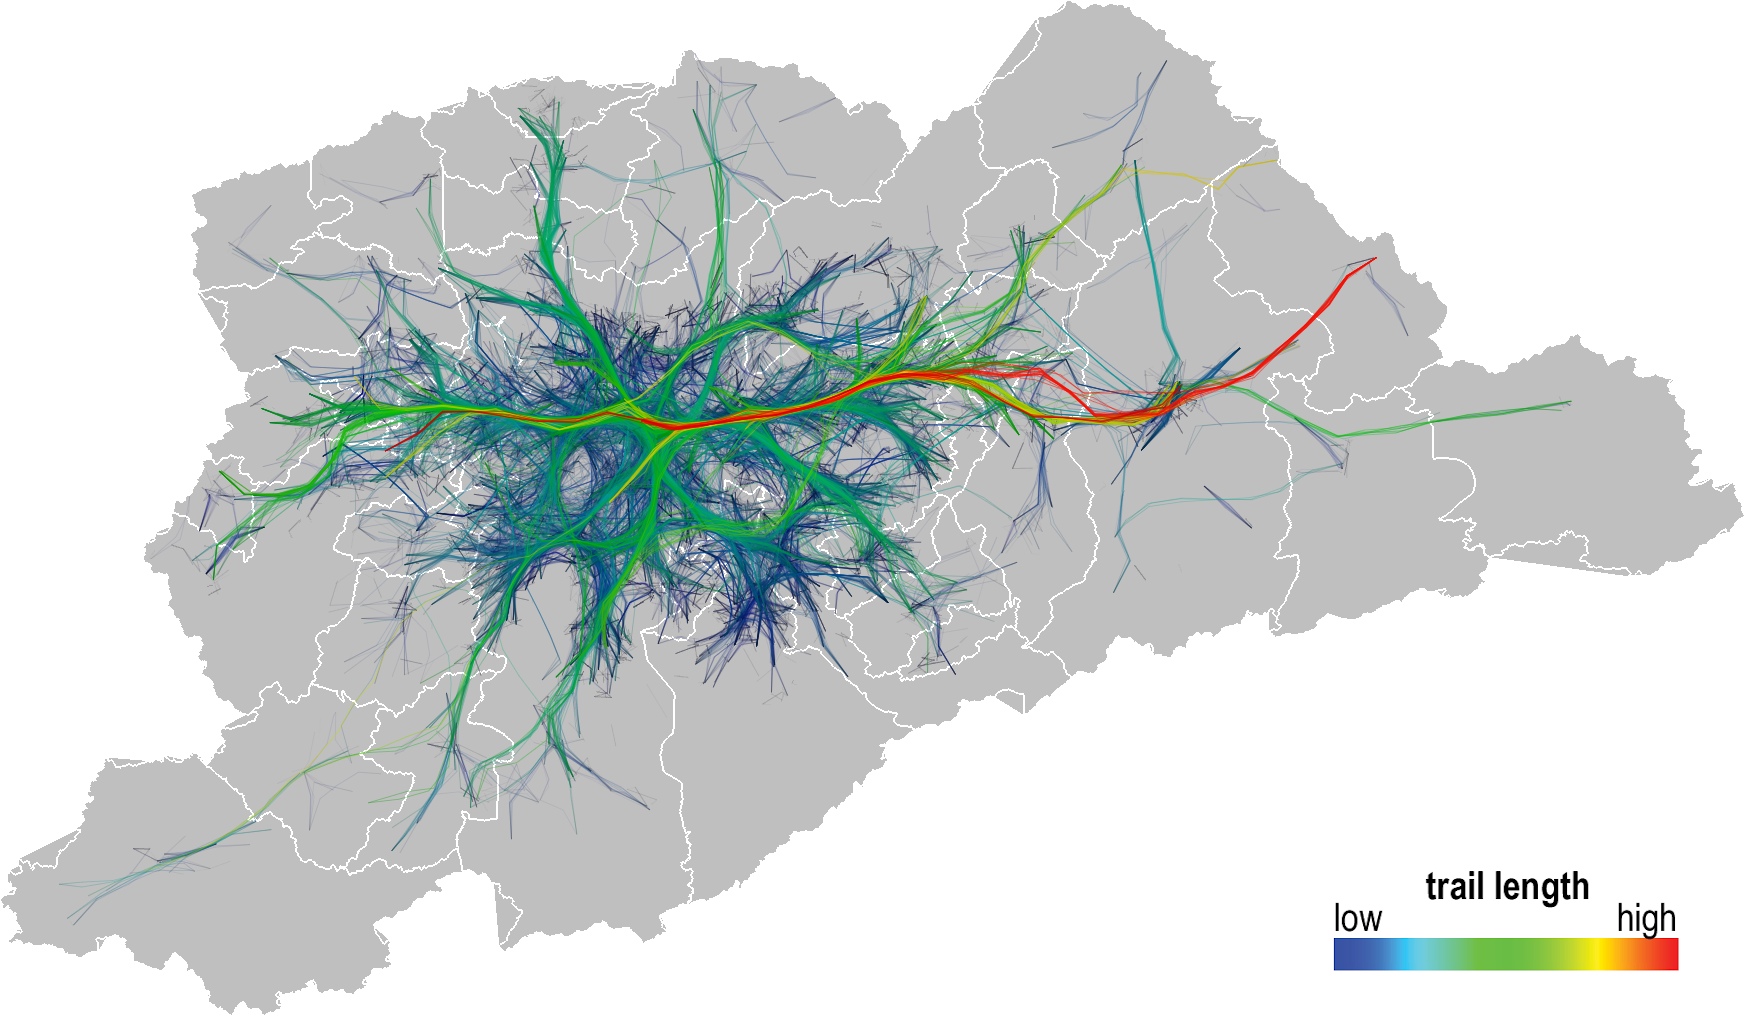
\includegraphics[width=0.98\textwidth]{../figuras/reason-school-leg.png}
\caption{Distâncias das viagens por motivo educação.\label{fig:reason-education}}
\end{figure}

\begin{figure}[!htb]
\centering
\captionsetup{justification=centering}
\includegraphics[width=0.98\textwidth]{../figuras/reason-shopping-leg.png}
\caption{Distâncias das viagens por motivo compras.\label{fig:reason-shopping}}
\end{figure}


% \par

\chapter{Resultados}
\label{sec:results}

Essa seção apresenta os resultados das análises que desenvolvemos sobre os dados
da pesquisa OD 17. Começamos com a exploração dos recursos de visualização
oferecidos pelo \emph{CUBu}, com ênfase na codificação visual dos atributos
densidade, distância e direção das viagens. Esses aspectos são apresentados a
seguir nas
Seções~\ref{sec:density},~\ref{sec:trail-overlap},~\ref{sec:length-direction},~e~\ref{sec:coloring}.
Posteriormente, utilizando tais recursos visuais analisamos outros padrões de
mobilidade específicos a subconjuntos dos dados, detalhados nas
Seções~\ref{sec:strata},~\ref{sec:students},~\ref{sec:peak-hours},~\ref{sec:dist_reasons},~e~\ref{sec:mode}.

\section{Visualizando a densidade dos \emph{bundles}}
\label{sec:density}

Na Seção~\ref{sec:bundling}, explicamos como a operação de \emph{bundling}
faz o agrupamento de trajetórias simplificando a visualização e reduzindo a oclusão
da imagem. No entanto, tal operação não nos diz quantas trajetórias foram agrupadas em
um \emph{bundle}. A solução para isso, primeiramente apresentada por \citet{holten06},
é desenhar linhas semi-transparentes, cada uma com uma transparência fixa $\alpha < 1$.
Assim, a combinação mostrará trajetórias de alta densidade como mais opacas e as de baixa
densidade como mais transparentes. Apesar da transparência ajudar na diferenciação
de áreas densas, ela por si só não é uma variável visual quantitativa forte \citep{slocum09}.
Então, codificamos também a densidade das trajetórias em cores, utilizando
os valores estimados pelo KDE durante o processo de \emph{bundling} (ver Seção~\ref{sec:bundling}).
A Figura~\ref{fig:bundled-graph-density}a mostra uma visualização obtida usando codificação
da densidade em cores aplicada em todo o conjunto de dados da OD17 contendo
as \num{685115} viagens. Podemos ver alguns caminhos com maior densidade, mas a imagem
ainda apresenta uma demasiada carga de informação e muitas áreas opacas. Isso ocorre pelo fato de que,
usualmente em GPUS de consumo comum, a transparência $\alpha$ é modelada por um valor
inteiro de 8 bits. Portanto, apenas 255 níveis de transparência diferentes são possíveis,
ou seja, apenas 255 níveis de densidade das trajetórias podem ser exibidos. Valores
de $\alpha$ muito altos saturam o canal de transparência
onde ocorrem as densidades mais altas - todas as densidades acima de 255 são fixadas
em 255. Valores abaixo de 1/255 resultam em nenhuma imagem, uma vez que
isso corresponde a opacidade zero na representação de 8 bits.

Para resolver este problema, mapeamos a densidade $\rho$ de duas maneiras,
transparência e cor. Já que $\rho$ é calculado precisamente como um número
de ponto flutuante durante a estimação do KDE, nenhum valor é truncado ou arredondado.
Essa estimativa da densidade permite modular a transparência para destacar ainda
mais as áreas de alta densidade e reduzir a oclusão da imagem. Uma outra alternativa
seria utilizar valores maiores de \emph{kernel} $k$, o que agruparia ainda mais as trajetórias, gerando
\emph{bundles} mais fortes, porém também iria causar uma maior distorção das linhas.
A Figura~\ref{fig:bundled-graph-density}b mostra o \emph{bundling} aplicado nos mesmos
dados da Figura~\ref{fig:bundled-graph-density}a. Podemos observar que os \emph{bundles}
aparecem mais salientes após aplicar a modulação da transparência. A imagem sugere que a rede do tráfego metropolitano
pode ser dividida em algumas ramificações principais que são fortemente conectadas à área central,
onde a cidade de São Paulo está localizada. Isso faz sentido considerando que esta é a parte
mais populosa da área metropolitana. Além disso, a maioria dos sistemas de transporte
cruzam o centro da capital, incluindo linhas de metrô, trem, e as principais vias expressas.

\begin{figure}[!htb]
  \centering
  \captionsetup{justification=centering}
  \includegraphics[width=0.98\textwidth]{../figuras/figure1}
  \caption{\emph{Bundling} das trajetórias coloridas pela densidade (a) valores fixos e \\(b) transparência modulada.}
  \label{fig:bundled-graph-density}  
\end{figure}

% % How we calculated 44%:
% %
% % 1. Take all trips that indicate bus, metro, and train as
% %    the main transportation mode -> this is the amount of
% %    trips by public transportation
% %
% % 2. Take all trips that indicate use of metro or train for
% %    some portion of the trip and divide that by the amount
% %    of trips by public transportation
% %
% % Using the tables from pages 46 and 49 of
% % http://www.metro.sp.gov.br/pesquisa-od/arquivos/Ebook%20Pesquisa%20OD%202017_final_240719_versao_4.pdf
% %
% % We consider that:
% % trips using bus as the main transportation mode: 8034
% % trips using train as the main transportation mode: 1245
% % trips using metro as the main transportation mode: 3400
% % total trips by public transportation: 8034 + 1245 + 3400 = 12679
% %
% % trips using metro for some portion of the trip: 3400
% % trips using train for some portion of the trip: 2272
% % total trips involving train or metro: 3400 + 2272 = 5672
% %
% % Percentage = 5672*100/12679 = 44.73%
% %
% % Not relevant for the text, just a curiosity:
% % the percentage in relation to all motorized trips is 5672*100/28280=20.05%

\section{Infraestrutura de metrô e trem \emph{vs.} \emph{bundling}}
\label{sec:trail-overlap}

O sistema de transporte público é o mais utilizado pelos moradores da RMSP. O
impacto da malha ferroviária sobre o deslocamento de pessoas fica claro quando
desenhamos as linhas ferroviárias ao longo das trajetórias agrupadas com o
\emph{bundling}. A Figura~\ref{fig:rails} mostra a alta correspondência dos
\emph{bundles} com os caminhos das linhas ferroviárias (desenhadas em preto).
Tendo em vista que, de acordo com a pesquisa OD17, cerca de 44\% das viagens
diárias de transporte público envolvem metrô ou trens, este é um resultado
esperado. Curiosamente pode-se questionar se o sistema ferroviário foi planejado
com precisão para atender a demanda, como sugere a visualização agrupada, ou se
a disponibilidade dessa opção de transporte influenciou a existência de fluxos
tão densos. Embora não temos os insumos para responder a essa pergunta, os
gestores de tráfego podem usar esse tipo de visualização para elaborar políticas
para o transporte público. Apesar de não expressar nenhuma grande surpresa sobre os
dados analisados, este é um resultado bastante importante, pois consideramos que a alta
correlação entre o \emph{bundling} das trajetórias e as linhas das ferrovias
também indica boas configurações de parâmetros para esse tipo de visualização na
escala da região metropolitana.

Ressaltamos que que este tipo de correlação (de \emph{bundles} com estradas) não
é o mesmo que o utilizado no método RAEB \citep{zeng:19}. No método RAEB, o
agrupamento foi feito explicitamente para seguir estradas. Em nosso caso, as
linhas são sobrepostas sobre \emph{bundles}, que foram gerados unicamente a partir dos
dados da OD. Pode-se argumentar que RAEB, neste sentido, produz \emph{bundles}
mais ``corretos'', uma vez que estes são forçados para seguir as estradas. No
entanto, olhando mais de perto, podemos ver que RAEB não pode ter todos os
\emph{bundles} seguindo precisamente todos os caminhos das estradas - pois isso
basicamente bloquearia qualquer agrupamento do \emph{bundling} e resultaria no próprio
mapa das estradas. Além disso, RAEB requer que o registro dos pontos das trajetórias
seja feito dentro de uma rede rodoviária precisa. Isso torna-o
significativamente mais complexo para implementar e mais caro para processar do
que nossa solução baseada em \emph{CUBu}.

\begin{figure}[!htb]
  \centering
  \captionsetup{justification=centering}
  \includegraphics[width=0.98\textwidth]{../figuras/rail-lines.png}
    \caption{\emph{Bundling} das trajetórias coloridas pela densidade e a malha ferroviária da RMSP}
  \label{fig:rails}  
\end{figure}

\section{Mapeando distância e direção no \emph{bundling}}
\label{sec:length-direction}

Para explorar a mobilidade urbana por diferentes perspectivas, precisamos de
meios para visualizar os múltiplos atributos dos dados. Dois
importantes atributos para o estudo de padrões de mobilidade são distância
percorrida na viagem e a sua direção. As Figuras~\ref{fig:attributes-length} e
\ref{fig:attributes-direction} mostram a visualização de todo o conjunto de
dados OD17 mapeando a distância e direção, respectivamente.

Na Figura~\ref{fig:attributes-length} codificamos nas cores os comprimentos das
viagens. Nela utilizamos o mesmo mapa de cores (arco-íris) da
Figura~\ref{fig:rails}, além também de aplicar a modulação da transparência por densidade,
conforme explicado na Seção~\ref{sec:density}. Nesta imagem, podemos observar
uma única curva vermelha aparentemente na horizontal. Sua alta opacidade implica
que há muitas viagens longas, todas mapeadas perfeitamente para essa trajetória
entre a mesma origem e destino (se não o fizessem, veríamos um \emph{bundle} se
ramificando no formato de um leque em vez de uma curva precisa). Esta é uma
descoberta interessante que, argumentamos, não poderia ser facilmente encontrada
usando métodos não visuais. Apesar desse ponto fora do comum, as outras trajetórias,
em geral, percorrem distâncias regulares. \emph{Bundles} de longa distância como
este podem indicar falta de serviços ou recursos que não satisfazem as regiões
locais, obrigando as pessoas a percorrerem longas distâncias para acessá-los. A
pesquisa OD17 contém mais informações que podem ajudar a investigar o motivo
dessas longas viagens.

A Figura~\ref{fig:attributes-direction} mostra os mesmos dados da
Figura~\ref{fig:attributes-length}, mas ao invés da distância são as direções
das viagens que estão codificadas em cores. Para este atributo em específico,
usamos ainda um recurso do \emph{CUBu}, que separa trilhas em direções opostas
em dois \emph{bundles} quase paralelos. Podemos ver claramente a existência de
trajetórias paralelas ao longo dos \emph{bundles}, o que não é surpreendente
porque a pesquisa OD registra o trajeto típico das pessoas que inclui os
deslocamentos de ida e vinda de volta para suas origens. No entanto, essa
simetria das trajetórias não é observada quando analisamos períodos
específicos do dia, como mostramos na Seção~\ref{sec:peak-hours}.

\begin{figure}[!htb] \centering \captionsetup{justification=centering}
  \includegraphics[width=0.98\textwidth]{../figuras/distances.png}
  \caption{Mapeamento da distância das viagens em cores. \label{fig:attributes-length}}
  \end{figure}

\begin{figure}[!htb]
  \centering
  \captionsetup{justification=centering}
  \includegraphics[width=0.98\textwidth]{../figuras/directions.png}
  \caption{Mapeamento da direção das viagens em cores. \label{fig:attributes-direction}}
\end{figure}

\section{Visualização dos modos de transporte: ônibus locais \emph{vs.} intermunicipais}
\label{sec:coloring}

Como mostramos na Seção~\ref{sec:pesquisa-od}, o conjunto de dados OD17 contém
17 modos de transporte. Embora fosse ideal ser capaz de ver as 17 categorias ao
mesmo tempo em nossa visualização com \emph{bundling}, isso não seria fácil de
se obter, uma vez que exigiria a codificação simultânea de 17 diferentes
categorias de transporte. Então, nós utilizamos a transparência para esconder
trajetórias de acordo com seletores que podem ser configurados na interface para
filtrar as trajetórias pelo modo de transporte, como mostra a Figura~\ref{fig:filtros-modes}
a seguir.

\begin{figure}[!h]
  \centering
  \includegraphics[width=.27\textwidth]{../figuras/filtros-modes.png}
  \caption{Filtros de transparência na interface do \emph{CUBu} para seleção dos modos de transporte.}
   \label{fig:filtros-modes}
 \end{figure}

Assim, na Figura~\ref{fig:bus-integration} mostramos como utilizamos tais
filtros que utilizamos para visualizar a integração entre os ônibus da cidade de
São Paulo (ônibus locais) e os ônibus intermunicipais. As trajetórias originais
e agrupadas com \emph{bundling} são apresentadas lado a lado. Cada meio de
transporte tem uma coloração distinta - verde para ônibus locais e azul para
ônibus intermunicipais. Podemos ver mais claramente na
Figura~\ref{fig:bus-integration-zoom} (zoom) que esses diferentes sistemas de
transporte parecem se complementar. A cidade de São Paulo tem um comércio e uma
indústria muito ativa, que recebe muitos trabalhadores advindos das cidades
vizinhas. Assim, a disponibilidade de transporte público e sua integração é
muito importante para essas pessoas. Esse tipo de filtragem juntamente com as
técnicas de \emph{bundling} ajudam a entender melhor as correlações entre os
atributos dos dados - neste caso, modos de transporte.


\begin{figure}[!htb]
  %\centering
  %\raggedright\noindent\hspace{-\margemesq}\hspace{.01\paperwidth}%
  %\begin{subfigure}{0.49\paperwidth}
  \raggedright\noindent\hspace{-.02\textwidth}%
  \begin{subfigure}{0.55\textwidth}
    \centering
    \includegraphics[width=1\textwidth]{../figuras/busesLocalXmetropolitan/unbundled-buses.png}
    \caption{\label{fig:bus-integration-a}}
  \end{subfigure}\nobreak%
  %\begin{subfigure}{0.49\paperwidth}
  \hspace{-.06\textwidth}\nobreak%
  \begin{subfigure}{0.55\textwidth}
    \centering
    \includegraphics[width=1\textwidth]{../figuras/busesLocalXmetropolitan/bundled-buses-length.png}
    \caption{\label{fig:bus-integration-b}}
  \end{subfigure}

  %\noindent\hspace{-\margemesq}\hspace{.01\paperwidth}\begin{subfigure}{0.49\paperwidth}
  \raggedright\noindent\hspace{-.02\textwidth}%
  \begin{subfigure}{0.55\textwidth}
    \centering
    \includegraphics[width=1\textwidth]{../figuras/busesLocalXmetropolitan/unbundled-metropolitan-buses.png}
    \caption{\label{fig:bus-integration-c}}
  \end{subfigure}\nobreak%
  \hspace{-.06\textwidth}\nobreak%
  \begin{subfigure}{0.55\textwidth}
  %\begin{subfigure}{0.49\paperwidth}
    \centering
    \includegraphics[width=1\textwidth]{../figuras/busesLocalXmetropolitan/bundled-metropolitan-buses-length.png}
    \caption{ \label{fig:bus-integration-d}}
  \end{subfigure}

  %\noindent\hspace{-\margemesq}\hspace{.01\paperwidth}\begin{subfigure}{0.49\paperwidth}
  \raggedright\noindent\hspace{-.02\textwidth}%
  \begin{subfigure}{0.55\textwidth}
    \centering
    \includegraphics[width=1\textwidth]{../figuras/busesLocalXmetropolitan/unbundled-buses-and-metropolitan.png}
    \caption{\label{fig:bus-integration-e}}
  \end{subfigure}\nobreak%
  \hspace{-.06\textwidth}\nobreak%
  \begin{subfigure}{0.55\textwidth}
  %\begin{subfigure}{0.49\paperwidth}
    \centering
    \includegraphics[width=1\textwidth]{../figuras/busesLocalXmetropolitan/bundled-buses-and-metropolitan-length.png}
    \caption{\label{fig:bus-integration-f}}
  \end{subfigure}
  \caption{Viagens filtradas pelo modo de transporte: ônibus locais e intermunicipais. Dados originais à esquerda (a, c, e)  e \emph{bundling} à direita (b, d, f). \label{fig:bus-integration}}
\end{figure}

\begin{figure}[!htb]
  \centering
  \captionsetup{justification=centering}
  \includegraphics[width=0.98\textwidth]{../figuras/local-intercity-buses}
  \caption{Viagens filtradas pelo modo de transporte: ônibus locais e intermunicipais (zoom). \label{fig:bus-integration-zoom}}
\end{figure}

\section{Visualização das diferentes classes sociais}
\label{sec:strata}

Usamos nossa visualização com \emph{bundling} para estudar como os cidadãos com diferentes
condições econômicas se deslocam na RMSP. O Critério de Classificação Econômica
Brasileira (CCEB), \citep{cceb2008} é o índice socioeconômico oficial utilizado no Censo
Demográfico Brasileiro, realizado pelo Instituto Brasileiro de Geografia e
Estatística (IBGE). Ele mede o poder de compra da sociedade brasileira. O CCEB é
dividido em seis níveis (ou classes) (Tabela~\ref{tab:becc}). Este índice é usado na pesquisa
OD17 para complementar os dados de mobilidade. A Tabela~\ref{tab:becc} também mostra a renda
média mensal (em reais), e o número de viagens na RMSP para cada nível do CCEB considerando toda a população e apenas
os cidadãos com idade entre 6 e 18 anos que se deslocam para fins de estudos (consulte a
Seção~\ref{sec:students}). O motivo pelo qual o total de viagens na tabela ser abaixo de 42 milhões
é que muitos registros do conjunto de dados não tinham a informação da sua classificação no CCEB, e por isso
não foram considerados no cálculo.

\begin{table}[!htb]
  \small
  \newcommand{\hdr}[1]{\bfseries#1}
  \centering
  \caption{Quantidade de viagens pelo índice CCEB (2017), renda mensal e idade. \label{tab:becc}}
  \begin{tabular}{>{\footnotesize}c>{\footnotesize}r>{\footnotesize}r>{\footnotesize}r>{\footnotesize}r}
    \toprule
    \multirow{2}[2]{*}{\hdr{Nível CCEB}} & \hdr{Renda mensal} & \hdr{Viagens} & \hdr{Viagens de estudantes}\\
    & \hdr{em reais (R\$)} & \hdr{totais} & \hdr{entre 6 e 18 anos}\\
    \midrule
    A   & 23,345    & 3,062,892  &   184,772\\
    B1  & 10,386    & 3,854,040  &   260,652\\
    B2  & 5,363     & 12,856,182 &   963,242\\
    C1  & 2,965     & 11,277,159 &   976,745\\
    C2  & 1,691     & 7,852,806  &   721,218\\
    D-E & 708       & 2,233,801  &   219,612\\
    \textbf{Total}& n/a & 411,368,80 &  3,326,241\\
    \bottomrule
  \end{tabular}
\end{table}

Para comparar os padrões de mobilidade de diferentes classes sociais CCEB,
aplicamos \emph{bundling} nas viagens de cada classe separadamente, como
mostrado nas Figuras~\ref{fig:becc-axd-e}~até~\ref{fig:becc-d-e}. Observamos
diferenças significativas nos padrões de mobilidade entre os níveis de renda
mais altos e mais baixos, como mostra a Figura~\ref{fig:becc-axd-e}. O nível $A$
(Figura~\ref{fig:becc-a}) apresenta alta densidade no centro da RMSP, que inclui
o entorno do centro da capital. A maior densidade está localizada nos bairros
oeste, sudoeste e nordeste próximos ao centro. Existem fluxos de densidade entre
a capital e as cidades de Barueri e Cotia, que possuem áreas residenciais de
alta renda. Existem outros fluxos de alta densidade ligando a capital às cidades
de São Bernardo do Campo e Santo André. Comparando A ao nível D-E (Figura 18),
vemos que D-E tem os fluxos densos mais elevados na região leste da capital. No
mapa de níveis D-E, podemos ver a ausência de fluxos de alta densidade nas
regiões mais próximas do centro da capital; em contraste, eles estão presentes
no mapa de nível A.

\begin{figure}[!htb]
  \centering
  \captionsetup{justification=centering}
  \includegraphics[width=0.98\textwidth]{../figuras/comparison-axd-e-strata-leg.png}
  \caption{Densidade das viagens da classe $A$ (esquerda) e $D$-$E$ (direta). \label{fig:becc-axd-e}}
\end{figure}

\begin{figure}[!htb]
  \centering
  \captionsetup{justification=centering}
  \includegraphics[width=0.98\textwidth]{../figuras/1-class-a.png}
  \caption{Densidade das viagens da classe $A$. \label{fig:becc-a}}
\end{figure}

\begin{figure}[!htb]
  \centering
  \captionsetup{justification=centering}
  \includegraphics[width=0.98\textwidth]{../figuras/2-class-b1.png}
  \caption{Densidade das viagens da classe $B1$. \label{fig:becc-b1}}
\end{figure}

\begin{figure}[!htb]
  \centering
  \captionsetup{justification=centering}
  \includegraphics[width=0.98\textwidth]{../figuras/3-class-b2.png}
  \caption{Densidade das viagens da classe $B2$. \label{fig:becc-b2}}
\end{figure}

\begin{figure}[!htb]
  \centering
  \captionsetup{justification=centering}
  \includegraphics[width=0.98\textwidth]{../figuras/4-class-c1.png}
  \caption{Densidade das viagens da classe $C1$. \label{fig:becc-c1}}
\end{figure}

\begin{figure}[!htb]
  \centering
  \captionsetup{justification=centering}
  \includegraphics[width=0.98\textwidth]{../figuras/5-class-c2.png}
  \caption{Densidade das viagens da classe $C2$. \label{fig:becc-c2}}
\end{figure}

\begin{figure}[!htb]
  \centering
  \captionsetup{justification=centering}
  \includegraphics[width=0.98\textwidth]{../figuras/6-class-d-e.png}
  \caption{Densidade das viagens da classe $D$-$E$. \label{fig:becc-d-e}}
\end{figure}

Quando comparamos todos os mapas do nível $A$ ao $D-E$
(Figuras~\ref{fig:becc-a}~to~\ref{fig:becc-d-e}), vemos que os fluxos mais
densos (em vermelho) tendem a se deslocar do centro da capital para a região
leste da cidade. A concentração de fluxos de alta densidade está se espalhando
cada vez mais do centro para as regiões periféricas da RMSP. Mesmo os fluxos
menos densos também se espalham pela RMSP. No entanto, o mapa $D-E$ mostra que
esses fluxos diminuem consideravelmente (podemos ver pelas linhas menos densas)
para essas classes sociais. Isso pode indicar que os cidadãos de baixa renda
têm menos acesso ao sistema de mobilidade urbana. Com isso, essas pessoas teriam
menos acesso aos serviços sociais, educacionais, de saúde e culturais da RMSP,
uma vez que esses recursos estão concentrados nas regiões centrais das cidades.
É importante notar que essas regiões centrais também têm mais oportunidades de
emprego. Olhando o mapa $D-E$, podemos ver um notável espaço vazio no centro
oeste da capital. Essa região (distrito de Pinheiros) concentra um grande número
de empregos relacionados à tecnologia da informação e serviços financeiros, o
que requer trabalhadores com níveis de escolaridade alto e médio. Assim, o mapa
mostra que os cidadãos de baixa renda não estão indo para aquela região, o que
reflete a desigualdade de oportunidades que esses cidadãos enfrentam.

\section{Mobilidade de jovens estudantes de diferentes classes sociais}
\label{sec:students}

Um outro uso do \emph{bundling} que fizemos em nosso estudo de visualização de padrões de
mobilidade foi para comparar as viagens de estudantes de diferentes classes
sociais. Para isso, filtramos viagens de indivíduos com idades entre 6 e 18 anos
cujo motivo do deslocamento é o estudo. Então, nós os dividimos em dois grupos,
de alta a moderada renda, que inclui os níveis CCEB $A$, $B1$, $B2$ e $C1$; e os
de baixa renda, que incluem os níveis $C2$ e $D$ - $E$. As
figuras~\ref{fig:students-high}~e~\ref{fig:students-low} mostram os mapas de
densidade para ambos os grupos.

\begin{figure}[!htb]
  \centering
  \captionsetup{justification=centering}
  \includegraphics[width=0.98\textwidth]{../figuras/high-income-density-leg.png}
  \caption{Densidade das viagens de estudantes de alta renda. \label{fig:students-high}}
\end{figure}
\vspace*{\floatsep}
\begin{figure}[!htb]
  \centering
  \captionsetup{justification=centering}
  \includegraphics[width=0.98\textwidth]{../figuras/low-income-density-leg.png}
  \caption{Densidade das viagens de estudantes de baixa renda. \label{fig:students-low}}
\end{figure}

Podemos ver no mapa da Figura~\ref{fig:students-high} que a densidade dos fluxos
do grupo de alunos de alta a moderada renda se mostram muito mais densos e
espalhados pela a região central da RMSP. Esta parte da RMSP concentra a maioria
das escolas particulares, universidades e faculdades. Já o mapa de densidade de
alunos de baixa renda (Figura~\ref{fig:students-low}) mostra uma mobilidade bem
mais limitada em comparação com os alunos de alta renda, com alguns fluxos
interligados ao centro da capital, mas a maioria dos fluxos densos dessa classe
estão mais presentes nas periferias da capital e também nas cidades vizinhas.
Apesar das diferenças, podemos ver que há concentração dos dois grupos na região
sudoeste, onde ficam os bairros do distrito de Campo Limpo.

Podemos observar que há muito mais trilhas para os alunos de alta renda
(Figura~\ref{fig: students-high}) do que para alunos de baixa renda
(Figura~\ref{fig:students-low}). Os estudantes de renda alta também viajam
grandes distâncias para estudar, o que indica que podem escolher com mais
flexibilidade onde estudar. Este fato é corroborado por estudos de mobilidade
urbana que indicam que pessoas com melhores condições financeiras têm mais
mobilidade do que aquelas com condições mais precárias, como em \citet{carruthers2005,
lucas2016}.

Vale ressaltar que as escolas de ensino públicas   da RMSP estão distribuídas pela região
central e periférica das cidades. Em geral, o sistema público busca alocar as
matrículas dos alunos nessas escolas de acordo com a proximidade de suas
residências. Assim, eles não precisam viajar longas distâncias para chegar às
suas escolas. Além disso, as escolas públicas apresentam desempenho educacional
inferior ao das escolas particulares de São Paulo. Assim, cidadãos com melhores
condições financeiras costumam colocar seus filhos em escolas particulares,
padrão que se inverte no ensino superior.

A escassez de fluxos de alunos de baixa renda levanta questionamentos. Ela pode
ser uma indicação de que essa classe da população não tem oportunidades iguais
de estudo. Também não costumam ir para a região central da cidade e, portanto,
têm menos acesso a universidades e faculdades complementares. Essa desigualdade
de oportunidades provavelmente afetará os empregos e as condições econômicas
desses alunos.

\section{Direção das viagens nos horários de pico}
\label{sec:peak-hours}

Conforme mostramos anteriormente na Figura~\ref{fig:trips_by_hour} da
Seção~\ref{sec:pesquisa-od}, distribuição das viagens por hora do dia tem dois
picos principais, entre 6 e 9h e entre 17 e 20h. No entanto, essa tabela
agregada não fornece informações sobre como os padrões de mobilidade nos
horários de pico podem ser diferentes. Para visualizar esses dados aplicamos o
\emph{bundling} no conjunto de dados e então aplicamos um filtro que para
alterar a transparência das viagens fora do horário selecionado. Codificamos a
direção a das viagens em cores, similar ao apresentado na
Figura~\ref{fig:attributes-direction}, da Seção~\ref{sec:length-direction}.

\begin{figure}[!htb]
  \centering
  \captionsetup{justification=centering}
  \includegraphics[width=0.98\textwidth]{../figuras/peak-hours-6h-to-9h-direction-leg.png}
  \caption{Direção das viagens entre 6 e 9 da manhã. \label{fig:peak-hours-6h-9h}}
\end{figure}
\vspace*{\floatsep}
\begin{figure}[!htb]
  \centering
  \captionsetup{justification=centering}
  \includegraphics[width=0.98\textwidth]{../figuras/peak-hours-17h-to-20h-direction-leg.png}
  \caption{Direção das viagens entre 17 e 20h. \label{fig:peak-hours-17h-20h}}
\end{figure}

Comparando as horas de pico, podemos ver que os fluxos matinais indo para o
centro da RMSP (Figura~\ref{fig:peak-hours-6h-9h}, fluxo ciano vindo do leste)
são geralmente mais densos e mais longos do que os fluxos vindos do Centro RMSP
durante o pico da tarde/noite (Figura~\ref{fig:peak-hours-17h-20h}, fluxo
vermelho). Isso sugere que na manhã as pessoas têm um comportamento na ida ao
trabalho, ao passo que esse fluxo se distribui de maneira diferente na volta
para casa, possivelmente se designando para outros destinos (como escolas ou
academia) no período da tarde/noite. Um recurso interessante para esse tipo de
visualização é a separação das trajetórias em direções opostas alterando-se
diretamente o algoritmo de \emph{bundling}, como sugere \citet{adeb}. Em teoria,
sua técnica seria capaz de gerar agrupamentos mais nítidos levando em
consideração esse atributo. Porém, por questões de limite tempo e escopo deste
trabalho, não nos aprofundamos nesse tópico.

\section{Densidade das viagens por modo de transporte}
\label{sec:mode}

Um outro interessante atributo presente nos dados da pesquisa OD17 é o modo de
transporte. Comparamos então padrões de fluxo para quatro modos de transporte
diferentes: pedestres, bicicletas, carros e metrô. Nas
figuras~\ref{fig:mode-pedestrian}~até~\ref{fig:mode-subway} utilizamos o
\emph{bundling} para visualizar a densidade dos fluxos de cada um dos tipos de
transporte. Diferentemente do que apresentamos na seção~\ref{sec:coloring}, onde
aplicamos \emph{bundling} em todo o conjunto de dados e utilizamos filtros para
selecionar categorias de transporte de interesse, aqui utilizamos a estratégia de
particionamento para visualizar cada conjunto separadamente. Com isso damos
ênfase às características de cada subconjunto em específico, já que o
mapa de densidade é calculado com os valores daquela única classe de atributos.
 
\begin{figure}[!htb]
  \centering
  \captionsetup{justification=centering}
  \includegraphics[width=0.98\textwidth]{../figuras/mode-pedestrian-density-leg.png}
  \caption{Densidade das viagens de pedestres. \label{fig:mode-pedestrian}}
\end{figure}

\begin{figure}[!htb]
  \centering
  \captionsetup{justification=centering}
  \includegraphics[width=0.98\textwidth]{../figuras/mode-bike-density-leg.png}
  \caption{Densidade das viagens de bicicleta \label{fig:mode-bike}}
\end{figure}

\begin{figure}[!htb]
  \centering
  \captionsetup{justification=centering}
  \includegraphics[width=0.98\textwidth]{../figuras/mode-car-density-leg.png}
  \caption{Densidade das viagens de carro. \label{fig:mode-car}}
\end{figure}

\begin{figure}[!htb]
  \centering
  \captionsetup{justification=centering}
  \includegraphics[width=0.98\textwidth]{../figuras/mode-subway-density-leg.png}
  \caption{Densidade das viagens de metrô e trem. \label{fig:mode-subway}}
\end{figure}

As viagens de pedestres (Figura~\ref{fig:mode-pedestrian}) formam várias
``ilhas'' de baixa densidade espalhadas pela RMSP, sendo a mais densa (em vermelho)
no centro da capital. A maioria das trilhas são curtas, o que
é esperado para pedestres. No entanto, vemos alguns \emph{bundles} mais longos se estendendo
entre o centro da capital e as regiões sul e norte da cidade. Alguns fluxos mais densos também
estão presentes nas cidades vizinhas de Diadema, Taboão da Serra, Osasco,
Guarulhos, Poá e Mogi das Cruzes. Examinando mais de perto, observamos que
os fluxos densos combinam geograficamente com áreas centrais das cidades e as áreas comerciais. Essas
informações podem ser úteis para localizar locais que possam merecer a atenção
dos governos locais para proporcionar melhorias aos pedestres.

Como a maioria das viagens de pedestres são curtas, a técnica de \emph{bundling}
forma poucos fluxos sobre a RMSP. Usar o \emph{bundling} para essas viagens
curtas resulta em alguns poucos fluxos de baixa densidade, o que é menos útil em
comparação com viagens longas. Em casos como este, pode não ser necessário usar
o \emph{bundling}. Na área superior esquerda da
Figura~\ref{fig:mode-pedestrian}, temos destacadas as viagens OD da área central da
cidade sem utilização do \emph{bundling}; podemos ver que são quase idênticas
aos resultados com \emph{bundling} aplicado.

Com uma média de menos de três quilômetros, as viagens de bicicleta
(Figura~\ref{fig:mode-bike}) exibem padrões semelhantes aos de pedestres.  Nessa
figura, vemos alguns fluxos estreitos na área central da capital. Existem também
alguns fluxos mais salientes no Nordeste da capital e nas cidades vizinhas de
Suzano e Guarulhos. No entanto, comparando a Figura~\ref{fig:mode-bike} com
todos os outros meios de transporte, vemos imediatamente que as viagens de
bicicleta são de longe as menos numerosas e exibem um padrão muito mais esparso,
com poucos caminhos em forma de estrela onde muitas trajetórias se encontram.
Isso sugere que a infraestrutura de ciclismo em 2017 ainda era bastante limitada e fragmentada.
No canto superior esquerdo da Figura~\ref{fig:mode-bike} também mostramos
as viagens sem utilização do \emph{bundling}.

As viagens de carro (Figura~\ref{fig:mode-car}) mostram um padrão
semelhante ao que exibe todo o conjunto de dados, (ver Figura~\ref{fig:bundled-graph-density}).
Para começar, isso indica que os carros são a forma
dominante de transporte na RMSP, respondendo pelos principais padrões de
tráfego. Os fluxos de maior densidade ocorrem no centro da capital. Podemos observar diversos
fluxos de alta densidade ligando o Centro às demais regiões da capital, e também
indo e vindo das cidades de Guarulhos, Barueri, Cotia, São Bernardo do Campo,
Santo André, Mauá, e Mogi das Cruzes. Em comparação com todos os outros
modos de transporte, os carros mostram um padrão muito mais ``espalhado'' que
cobre áreas muito grandes, indicando que os carros são o modo de transporte
predominante na maioria das regiões da RMSP.

Por fim, as viagens de metrô e trem (Figura~\ref{fig:mode-subway}) apresentam um
forte padrão em forma de estrela, com fluxos de alta densidade que ligam a
capital às cidades vizinhas, devido à integração dos dois sistemas (vide
Seção~\ref{sec:trail-overlap}). Comparado aos outros modos de transporte, o
sistema de transporte de trilhos apresenta uma estrutura de padrão de viagem
mais clara e simples.

\section{Visualização por motivo da viagem}
\label{sec:dist_reasons}
Um outro atributo da pesquisa OD 17 que também achamos interessante em nossa
análise foi o motivo das viagens feitas. Observar a mobilidade urbana sobre essa
informação o pode revelar padrões comportamentais interessantes da população. A
seguir, estudamos as distâncias das viagens feitas por diferentes motivos, e que
tipos de padrões elas exibem. Para isso, criamos visualizações a partir dos
dados OD17 particionados por trabalho, saúde, educação e compras. As
figuras~\ref{fig:reason-work}~a~\ref{fig:reason-shopping} mostram os resultados.

As viagens de trabalho (Figura~\ref{fig:reason-work}) são geralmente mais longas
do que as outras razões de viagens e também cobrem uma área maior. Curiosamente, as viagens mais longas, entre o
lado leste e o centro da cidade (feixe vermelho), são um padrão semelhante às
viagens mais longas para saúde e educação. As viagens por motivos de saúde
(Figura~\ref{fig:reason-health}) são mais esparsas do que as relacionadas com o
trabalho e também apresentam um padrão mais estrelado, com longos fluxos
conectando-se à área central. Argumentamos que isso pode indicar que as regiões
periféricas não são bem servidas por serviços de saúde. As viagens por motivos
de estudo (Figura~\ref{fig:reason-education}) apresentam as maiores distâncias
entre as regiões Nordeste e Oeste da RMSP. Seu padrão apresenta ser algo
intermediário entre as viagens de trabalho e saúde. Curiosamente, as viagens
educacionais mostram várias ``voltas'' no centro da RMSP. Finalmente, as viagens
de compras (Figura~\ref{fig:reason-shopping}) mostram os padrões menos densos e,
em geral, também os mais curtos, mas com algumas exceções como o feixe vermelho
(importante) conectando o centro ao nordeste. Isso indica que, ao contrário da
saúde, educação e trabalho, os estabelecimentos comerciais (que na verdade são
da iniciativa privada) estão mais bem distribuídos na RMSP. Isso mostra que as
visualizações agregadas - como as feitas com \emph{bundling} - são úteis não
apenas quando mostram a \emph{presença} de certos dados, \emph{por exemplo}
viagens ligando regiões distantes; mas evidenciar a \emph{ausência} de padrões também
pode ser igualmente interessante.

\begin{figure}[!htb]
\centering
\captionsetup{justification=centering}
\includegraphics[width=0.98\textwidth]{../figuras/reason-work-leg.png}
\caption{Distâncias das viagens por motivo de trabalho.\label{fig:reason-work}}
\end{figure}
  
\begin{figure}[!htb]
\centering
\captionsetup{justification=centering}
\includegraphics[width=0.98\textwidth]{../figuras/reason-health-leg.png}
\caption{Distâncias das viagens por motivo de saúde.\label{fig:reason-health}}
\end{figure}

\begin{figure}[!htb]
\centering
\captionsetup{justification=centering}
\includegraphics[width=0.98\textwidth]{../figuras/reason-school-leg.png}
\caption{Distâncias das viagens por motivo educação.\label{fig:reason-education}}
\end{figure}

\begin{figure}[!htb]
\centering
\captionsetup{justification=centering}
\includegraphics[width=0.98\textwidth]{../figuras/reason-shopping-leg.png}
\caption{Distâncias das viagens por motivo compras.\label{fig:reason-shopping}}
\end{figure}



\chapter{Considerações Finais}
\label{cap:plano-de-trabalho}

Neste trabalho, exploramos o uso do \emph{bundling} para criar
visualizações de vários atributos dos dados de mobilidade urbana da Região
Metropolitana de São Paulo. Nossas análises sobre as características da pesquisa
OD 2017 mostram que o \emph{bundling} pode ser usado para identificar e comparar
diferentes padrões de mobilidade implícitos em diferentes subconjuntos de dados
e subconjuntos de atributos disponíveis. Combinando adequadamente a filtragem
(para reduzir a quantidade de dados e/ou atributos a serem explorados) com o
\emph{bundling} (para simplificar as visualizações criadas e reduzir a oclusão
visual) e com os canais visuais disponíveis (opacidade, cor, direção),
destacamos diferentes padrões no conjunto de dados OD17 que não teriam sido
facilmente obtido por ferramentas clássicas de mineração e visualização de
dados.

Nossos resultados sobre a visualização das trajetórias com \emph{bundling}
destacaram sua estrutura centralizada sobre a área estudada da RMSP. Além disso,
essa estrutura condiz com a infraestrutura metroviária e ferroviária de São
Paulo. Embora não tenha sido uma surpresa, a correlação sugere que nossos
parâmetros foram bem ajustados para a visualização na escala metropolitana.
Nossa metodologia para reduzir a complexidade do conjunto de dados de 42 milhões
de viagens para menos de um milhão, e também nossa adaptação de um
\emph{framework} de uso geral (CUBu) para agrupar subconjuntos específicos de
dados e/ou atributos foram os pontos principais que tornaram essa análise
possível. Desta forma conseguimos responder a nossa questão de pesquisa, pois
conseguimos obter um método de visualização de grandes conjuntos de dados de
mobilidade sob diferentes perspectivas e explorar seus múltiplos atributos.

Como trabalho futuro, pretendemos explorar melhorias no uso e usabilidade de
visualizações agregadas com \emph{bundling}. Do ponto de vista da visualização,
melhorias no mapa para mostrar as divisões das regiões no topo das trajetórias,
conforme proposto em \citet{Klein2014}, podem ajudar a identificar melhor as
conexões entre as regiões. Além disso, seria interessante testar uma abordagem
diferente para transmitir a informação de densidade dos \emph{bundles} alterando
a espessura das trajetórias proporcionalmente ao fator de expansão de cada
registro da OD17 em vez de usar cores, de forma semelhante a
\citet{lhuillier-fft:17}. Desta maneira não haveria a necessidade de replicar as
trajetórias como fizemos e, portanto, isso reduziria significativamente o
tamanho do conjunto de dados. Essas são etapas importantes para permitir o uso
de \emph{bundling} para análise em tempo real.

Da perspectiva da aplicação da técnica de \emph{bundling}, existem ainda muitas
outras possibilidades para análise da mobilidade urbana usando dados da própria
pesquisa OD e ainda a possibilidades de agregar outros conjuntos de dados, como
aqueles de empresas privadas de mobilidade, dispositivos IoT e sistemas de
compartilhamento de bicicletas. Há ainda espaço para se fazer uma análise
temporal mais profunda comparando a evolução da mobilidade urbana utilizando
dados das pesquisas OD anteriores. Por último, mas não menos importante, também
seria interessante complementar os resultados de nosso estudo com a avaliação de
usuários reais, como gestores de tráfego, para verificar a utilidade das
visualizações com \emph{bundling}.

% \section{Esforço Técnico}

% As colaborações deste trabalho envolveram também resultados técnic





\par
